%% $Id: bio_transport.tex,v 1.44 2007/04/22 13:50:54 benkirk Exp $
\chapter{Biological Transport\label{chap:bio}}

\section{Introduction}
Although the formation of spatial patterns is a central issue in biology the mechanisms which generate them are generally poorly understood.  Recent interdisciplinary collaboration has yielded mathematical models which capture the key biological processes involved in pattern formation and illustrate the unique roles played by different physical phenomenon.  These models generally consist of a coupled system of nonlinear partial differential equations.

Of particular interest in the present work is how local interactions produce global patterns in bacterial populations.  Such patterns have been observed experimentally by a number of researchers~\cite{berg_patterns_nature}, but only recently have mathematical models been developed which provide insight into how these patterns actually develop~\cite{spatial_patters_in_bio}.  Very complex patterns have been observed in colonies of \emph{Escherichia coli} (\emph{E.coli}) in a 0.24\% water agar semi--solid medium~\cite{berg_patterns_ecoli}.  Several experimentally observed patterns are presented in Figure~\ref{fig:ecoli_patterns_nature}.
\begin{figure}
  \begin{center}
    \subfigure{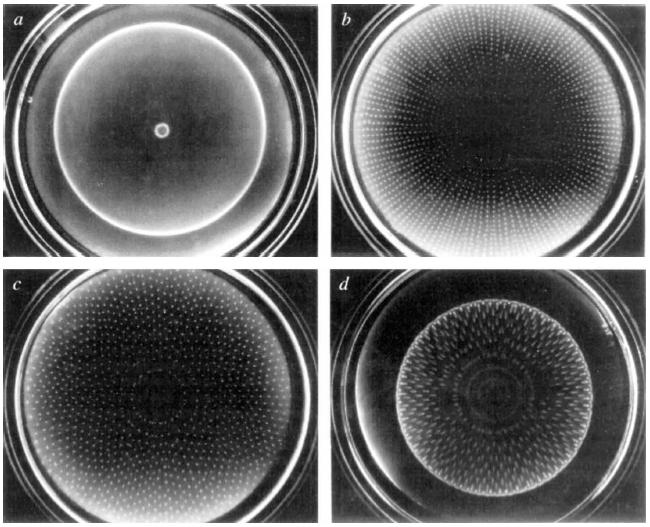
\includegraphics[width=.65\textwidth]{figures/budrene_berg/patterns}} \\
    \subfigure{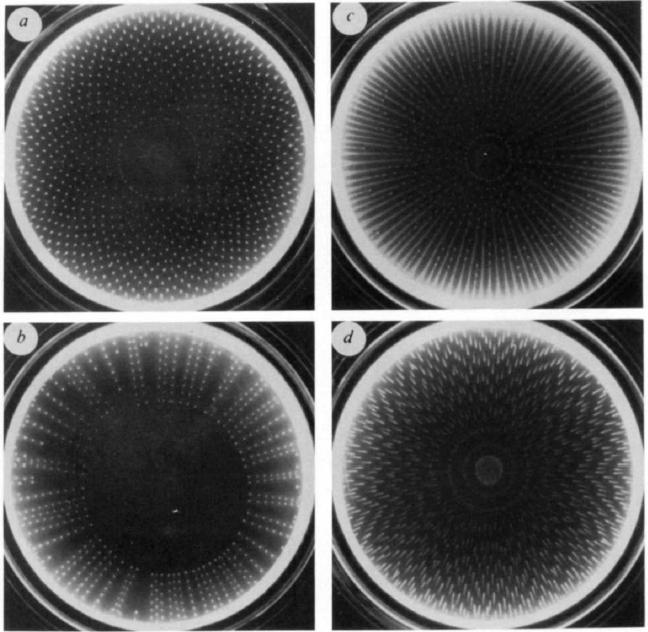
\includegraphics[width=.65\textwidth]{figures/budrene_berg/patterns2}}
    
    \caption[Pattern formation in \emph{E.coli}]{Pattern formation in \emph{E.coli}~\cite{berg_patterns_ecoli},\cite{berg_patterns_nature}\label{fig:ecoli_patterns_nature}}
  \end{center}
\end{figure}

The governing equations for this class of problems are of nonlinear reaction\---diffusion type and will be described in the following section.  These equations pose a number of challenges for accurate simulation including nonlinear coupling, rapid transients, and highly localized, transient features which must be addressed~\cite{staelens_thesis}.  It is interesting to note that while such features make this class of problems particularly well-suited for adaptive simulation techniques, there has been very little adaptive work for biological systems.  The goal of the present work is illustrate how the adaptive mesh refinement (AMR) techniques presented in Chapters~\ref{chap:amr} and~\ref{chap:parallel} can be used efficiently in a parallel environment to address this class of problems.  The use of adaptive techniques for this problem class enables high-resolution simulations of physical phenomena  that would be intractable with uniform meshes.  

%%%%%%%%%%%%%%%%%%%%%%%%%%%%%%%%%%%%%%%%%%%%%%%%%%%%%%%%%%%%%%%%%%%%%%%%%%%%%%%
\section{Mathematical Model}
\subsection{A Nonlinear Reaction-Diffusion Model for Chemotactic Systems}
\emph{E.coli} patterns are formed when the bacteria are exposed to an external stimulant, which can be thought of as a food source.  As a result of processing this stimulant the bacteria secrete aspartate, which is a strong chemoattractant.  This chemoattractant, in turn, induces chemotaxis, a process which essentially attracts bacteria.  The bacteria sense the ambient chemoattractant levels and move toward regions of higher concentration.   When chemotaxis is sufficiently strong it competes with diffusion and spatial patterns may develop.  Additionally, there are metabolic processes governing chemoattractant production and stimulant uptake which must be included in any model of such systems. Finally, the birth and death of bacteria must be modeled. This gives rise to a system for three variables: the cell density $n$, the chemoattractant concentration $c$, and the stimulant concentration $s$.  %Conceptually, these processes were combined by Murray et al.~\cite{spatial_patters_in_bio}.
The interplay of these physical processes is shown schematically in Figure~\ref{fig:conceptual_model}, and their mathematical treatment will now be discussed.
 \begin{figure}[hbpt]
   \begin{center}
     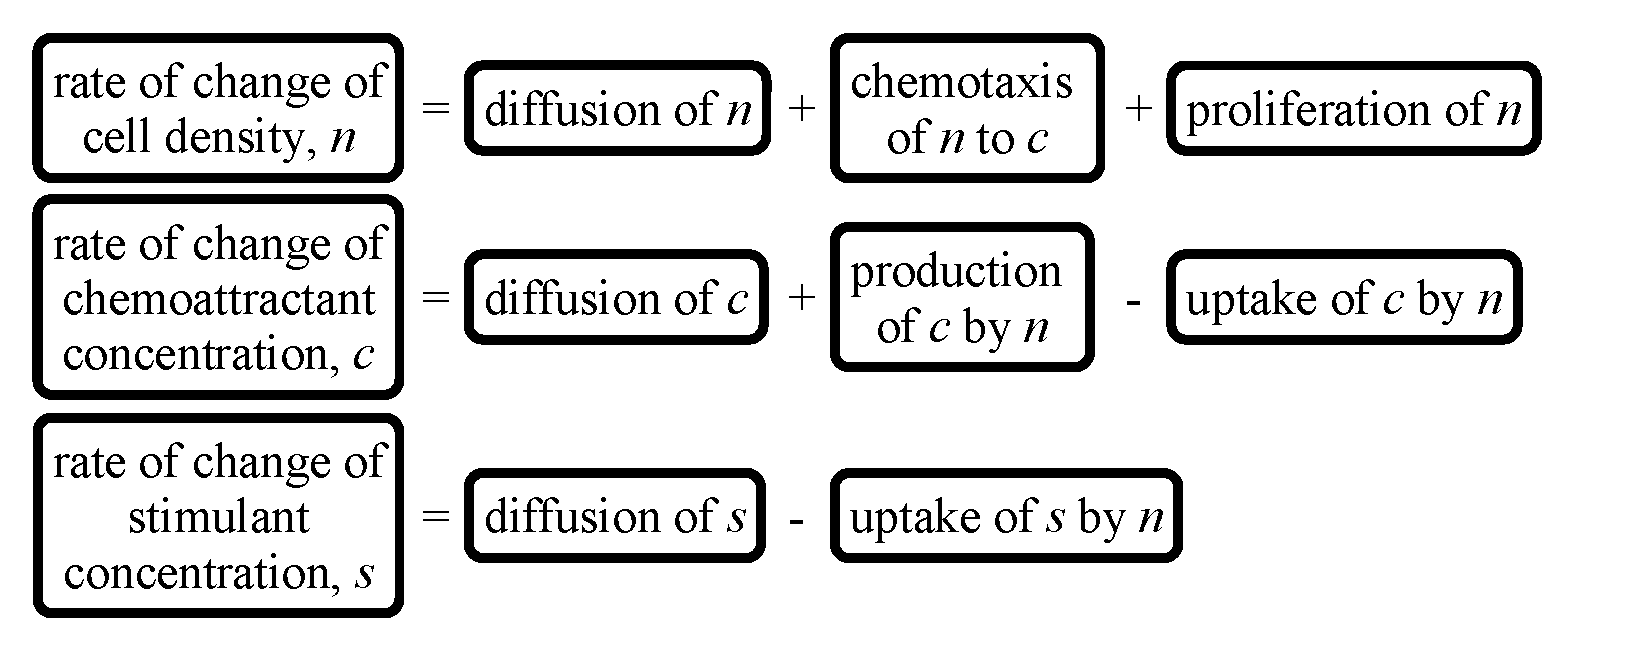
\includegraphics[width=\textwidth]{figures/bio/conceptual_model}
     \caption[Conceptual model of bacteria/chemoattractant/stimulant system.]{Conceptual model of bacteria/chemoattractant/stimulant system based on~\cite{spatial_patters_in_bio}.\label{fig:conceptual_model}}
   \end{center}
 \end{figure}

One possible mathematical model for bacterial chemotaxis is given by Murray et al.~\cite{spatial_patters_in_bio}:
% Bacterial chemotaxis: dimensional
\begin{align}
  \label{eq:pde_bio_n}
  \pdv{n}{t} & = D_n \Delta n - \grad{} \cdot \left[ \frac{k_1 n}{(k_2 + c)^2} \grad{c} \right]
                                    + k_3 n \left( k_4 \frac{s^2}{k_9 + s^2} - n \right) \\
  \label{eq:pde_bio_c}
  \pdv{c}{t} & = D_c \Delta c + k_5 s \frac{n^2}{k_6 + n^2} - k_7 nc \\
  \label{eq:pde_bio_s}
  \pdv{s}{t} & = D_s \Delta s - k_8 n \frac{s^2}{k_9 + s^2}
\end{align}
where $n$, $c$, and $s$ are the concentrations of bacteria, chemoattractant, and stimulant, respectively.  The remaining parameters govern the rates of proliferation, stimulant uptake, diffusion, and chemotaxis.  Some of these parameters have been measured experimentally, while others must be estimated. It should  be noted that the modeling of all right-hand-side terms in Equations~\eqref{eq:pde_bio_n}--\eqref{eq:pde_bio_s} other than diffusion is largely phenomenological in that other functional forms for these terms are plausible.  

Equation~\eqref{eq:pde_bio_n} describes the transport of bacteria.  The density of bacteria, $n$, may change through the physical processes of diffusion, chemotaxis, and proliferation.  These processes are described by the three terms on the right-hand-side of~\eqref{eq:pde_bio_n}.  Diffusion is the natural tendency for highly localized populations to spread out by moving in a direction away from the concentrated population (the direction opposite of the concentration gradient).  Conversely, chemotaxis is a process in which bacteria are attracted to regions of high chemoattractant density. In this case the bacteria move in the direction of increasing chemoattractant  (in the direction aligned with the chemoattractant gradient), hence chemotaxis may be thought of as an anti-diffusion process.  Finally, the proliferation of bacteria governs the growth or decay of a population in response to the local stimulant concentration. This term may be positive, negative, or zero depending on the local density of bacteria and stimulant.  In this way the proliferation term seeks to drive a given population into equilibrium with the available stimulant.

Equation~\eqref{eq:pde_bio_c} describes the transport of chemoattractant.  The three terms on the right-hand-side of the equation describe transport through diffusion, production, and depletion, respectively. The first term describes the familiar process of diffusion. The second term governs the production of chemoattractant which occurs when a bacteria concentration and stimulant are in contact.  This term is always positive or zero.  Conversely, the third term models depletion and may be negative or zero, depending upon local conditions.  This term represents the uptake of chemoattractant by bacteria.

Finally, Equation~\eqref{eq:pde_bio_s} governs the transport of stimulant.  In this model the local stimulant concentration may change through either diffusion or consumption.  There is no replenishing of stimulant in this model, although the degenerate case when $k_8=0$ corresponds to a fixed total amount of stimulant (for all time) whose spatial distribution may change only through diffusion.  In this case any initial stimulant distribution will tend to diffuse until it is distributed uniformly throughout the domain.

%\subsubsection{Nondimensionalization}
Equations~\eqref{eq:pde_bio_n}--\eqref{eq:pde_bio_s} can be scaled by introducing the following relationships~\cite{spatial_patters_in_bio}:
\\ %% 
\begin{minipage}[t]{.44\columnwidth}
  \begin{align}
    \hat{t} &= k_7 n_0 t \\
    u &= \frac{n}{n_0} \label{eq:bio_u_nondim}\\
    v &= \frac{c}{k_2} \\
    w &= \frac{s}{\sqrt{k_9}} \\
    \hat{\Delta} &= \frac{D_c}{k_7 n_0} \Delta \\
    d_u &= \frac{D_n}{D_c} \\
    d_w &= \frac{D_s}{D_c} 
  \end{align}
\end{minipage}
\hspace{.1\columnwidth}
\begin{minipage}[t]{.44\columnwidth}
  \begin{align}
    \alpha &= \frac{k_1}{k_2 D_c} \\
    \rho &= \frac{k_3}{k_7} \\
    \delta &= \frac{k_4}{n_0} \\
    \beta &= k_5 \frac{\sqrt{k_9}}{k_7 k_2 n_0} \\
    \kappa &= \frac{k_8}{k_7\sqrt{k_9}} \\
    \mu &= \frac{k_6}{n_0^2}
  \end{align}
\end{minipage}
\\
\\
which produces the nondimensional system
% Bacterial chemotaxis: nondimensional
\begin{align}
  \label{eq:pde_bio_u}
  \pdv{u}{\hat{t}} & = d_u \hat{\Delta} u - \alpha \grad{}\cdot \left[ \frac{u}{(1+ v)^2} \grad{v} \right]
                                    + \rho u \left( \delta \frac{w^2}{1 + w^2} - u \right) \\
  \label{eq:pde_bio_v}
  \pdv{v}{\hat{t}} & = \;\;\;\; \hat{\Delta} v + \beta w \frac{u^2}{\mu + u^2} - uv \\
  \label{eq:pde_bio_w}
  \pdv{w}{\hat{t}} & = d_w \hat{\Delta} w - \kappa u \frac{w^2}{1 + w^2}
\end{align}
For notational convenience the $\hat{()}$ will be dropped in the following sections.

%\subsubsection{Initial \& Boundary Conditions}
The initial conditions for the system are constructed to imitate a quiescent domain $\Omega$ with a given stimulant concentration $w_0$ at time $t=t_0$.  Since the domain initially is devoid of bacteria there is no initial chemoattractant concentration.  An initial inoculum of bacteria, $u_0$, is introduced and the solution evolves in response to this `disturbance.'  Specifically, for the problems that are considered subsequently
\begin{align}
  \label{eq:u0_bio}
  u_0 &= u(x,y), \;\; (x,y) \in \Omega \\
  \label{eq:v0_bio}
  v_0 &= 0 \\
  \label{eq:w0_bio}
  w_0 &= w(x,y), \;\; (x,y) \in \Omega
\end{align}
The actual implementation of initial conditions is an important issue.  Specifically, the initial conditions must be specified and implemented in a consistent way across a range of computational meshes.  This important aspect of the simulation will be addressed further in the application studies.

%\subsubsection{Boundary Conditions}
For a closed container with impermeable walls a physically sensible boundary condition for all variables in the system is 
\begin{align}
  \label{eq:du_dn_bio_eq_0}
  \pdv{u}{n} &= \grad{u}\cdot\nhat = 0 \\
  \label{eq:dv_dn_bio_eq_0}
  \pdv{v}{n} &= \grad{v}\cdot\nhat = 0 \\
  \label{eq:dw_dn_bio_eq_0}
  \pdv{w}{n} &= \grad{w}\cdot\nhat = 0
\end{align}
which simply states that there is no flux of bacteria, chemoattractant, or stimulant through the boundary of the domain~$\Omega$. %It will be seen in the following section that this boundary condition is particularly convenient to implement in the finite element discretization.



%%%%%%%%%%%%%%%%%%%%%%%%%%%%%%%%%%%%%%%%%%%%%%%%%%%%%%%%%%%%%%%%%%%%%%%%%%%%%%%
%\clearpage
\subsection{Weak Formulation}
The corresponding weighted-residual statement for equations~\eqref{eq:pde_bio_u}--\eqref{eq:pde_bio_v} follows from  multiplying each equation by a suitable test function~$\phi$ and integrating over the domain~$\Omega$, giving
\begin{align}
  \label{eq:weak_bio_u_preparts}
  \int_\Omega &\left[\pdv{u}{t} - d_u \Delta u + \alpha \grad{}\cdot \left[ \frac{u}{(1+ v)^2} \grad{v} \right]
                                    - \rho u \left( \delta \frac{w^2}{1 + w^2} - u \right)\right]\phi\dx  = 0 \\
  \label{eq:weak_bio_v_preparts}
  \int_\Omega &\left[\pdv{v}{t} - \Delta v - \beta w \frac{u^2}{\mu + u^2} + uv\right]\phi\dx = 0 \\
  \label{eq:weak_bio_w_preparts}
  \int_\Omega &\left[\pdv{w}{t} - d_w \Delta w + \kappa u \frac{w^2}{1 + w^2}\right]\phi\dx = 0
\end{align}
Applying Gauss' divergence theorem, selectively, and substituting \eqref{eq:du_dn_bio_eq_0}-\eqref{eq:dw_dn_bio_eq_0} in the resulting boundary integrals  yields the weak formulation: Find $\left(u,v,w\right)$ satisfying the specified initial conditions and
\begin{align}
  \int_\Omega& \left[\pdv{u}{t} - \rho u \left( \delta \frac{w^2}{1 + w^2} - u \right) \right]\phi\dx \nonumber \\
  \label{eq:weak_bio_u}
  &\;\;\;+ \int_\Omega \left[d_u \grad{u}\cdot\grad{\phi} - \alpha u \frac{\grad{v}\cdot\grad{\phi}}{(1+ v)^2} \right]\dx  = 0 \\  
  \label{eq:weak_bio_v}
  \int_\Omega& \left[\left(\pdv{v}{t} - \beta w \frac{u^2}{\mu + u^2} + uv\right)\phi + \grad{v}\cdot\grad{\phi}\right]\dx = 0 \\  
  \label{eq:weak_bio_w}
  \int_\Omega& \left[\left(\pdv{w}{t} + \kappa u \frac{w^2}{1 + w^2}\right)\phi + d_w\grad{w}\cdot\grad{\phi}\right]\dx = 0
\end{align}
for all admissible test functions $\phi$.  The weak statement~\eqref{eq:weak_bio_u}-\eqref{eq:weak_bio_w} implies \eqref{eq:pde_bio_u}-\eqref{eq:pde_bio_w} with \eqref{eq:du_dn_bio_eq_0}-\eqref{eq:dw_dn_bio_eq_0} as natural boundary conditions.
%This will starting point for the  finite element discretization discussed in the next section.

%Note that the boundary integrals in Equations~\eqref{eq:weak_bio_u}--\eqref{eq:weak_bio_w} (which result from integration by parts) have been omitted.  This is consistent with the no--flux boundary conditions imposed on the system.  Omitting these boundary integrals in~\eqref{eq:weak_bio_u}--\eqref{eq:weak_bio_w} naturally imposes these conditions in a weak sense.



%%%%%%%%%%%%%%%%%%%%%%%%%%%%%%%%%%%%%%%%%%%%%%%%%%%%%%%%%%%%%%%%%%%%%%%%%%%%%%%
\subsection{Finite Element Formulation}
The finite element formulation for~\eqref{eq:weak_bio_u}--\eqref{eq:weak_bio_w} follows upon replacing $\left(u,v,w\right)$ and $\phi$ with the finite dimensional approximations  $\left(u_h,v_h,w_h\right)$ and $\phi_h$.  Specifically, for a standard Lagrange finite element basis we have
\begin{align}
  \label{eq:bio_u_h}  
  u_h(\bv{x},t) &= \sum_{j=1}^N u_j(t) \phi_j(\bv{x}) \\
  \label{eq:bio_v_h}  
  v_h(\bv{x},t) &= \sum_{j=1}^N v_j(t) \phi_j(\bv{x}) \\
  \label{eq:bio_w_h}  
  w_h(\bv{x},t) &= \sum_{j=1}^N w_j(t) \phi_j(\bv{x}) 
\end{align}
where $u_j(t)$, $v_j(t)$, and $w_j(t)$ are the nodal values of the bacteria, chemoattractant, and stimulant at time $t$, respectively, and $N$ is the number of nodes in the domain. The corresponding discrete weak statement is then: find the approximate solution $\left(u_h,v_h,w_h\right)$ satisfying the specified initial conditions and 
\begin{align}
  \int_\Omega& \left[\pdv{u_h}{t} - \rho u_h \left( \delta \frac{w_h^2}{1 + w_h^2} - u_h \right) \right]\phi_h\dx \nonumber \\
  \label{eq:fe_bio_u}
  &\;\;\;+ \int_\Omega \left[d_u \grad{u_h}\cdot\grad{\phi_h} - \alpha u_h \frac{\grad{v_h}\cdot\grad{\phi_h}}{(1+ v_h)^2} \right]\dx  = 0 \\  
  \label{eq:fe_bio_v}
  \int_\Omega& \left[\left(\pdv{v_h}{t} - \beta w_h \frac{u_h^2}{\mu + u_h^2} + u_h v_h\right)\phi_h + \grad{v_h}\cdot\grad{\phi_h}\right]\dx = 0 \\ 
  \label{eq:fe_bio_w}
  \int_\Omega& \left[\left(\pdv{w_h}{t} + \kappa u_h \frac{w_h^2}{1 + w_h^2}\right)\phi + d_w\grad{w_h}\cdot\grad{\phi_h}\right]\dx = 0
\end{align}
for all admissible test functions $\phi_h$.  This discrete approximation to \eqref{eq:weak_bio_u}-\eqref{eq:weak_bio_w} forms the basis of the computational model described in the next section.


%%%%%%%%%%%%%%%%%%%%%%%%%%%%%%%%%%%%%%%%%%%%%%%%%%%%%%%%%%%%%%%%%%%%%%%%%%%%%%%
\section{Solution Methodology}
Equations~\eqref{eq:pde_bio_u}--\eqref{eq:pde_bio_w} form a highly coupled, transient,  nonlinear system.  Furthermore, the system evolution occurs over a disparate range of time scales that must be captured accurately.  This section outlines the techniques employed in the present work to solve the system of equations.

%%%%%%%%%%%%%%%%%%%%%%%%%%%%%%%%%%%%%%%%%%%%%%%%%%%%%%%%%%%%%%%%%%%%%%%%%%%%%%%
\subsection{Time Integration}
The time integration method used in this work can be developed by considering the generic first-order ordinary differential equation
\begin{equation}
  \label{eq:udot_eq_f_u}
  \bv{\dot{u}} = \bv{f}\left(t,\bv{u}\left(t\right)\right),\;\; t>t_0,\;\; \bv{u}\left(t_0\right) = \bv{u}_0
\end{equation}
Explicit methods for~\eqref{eq:udot_eq_f_u} are simple to formulate and the computational cost per step is low.  The price for this simplicity is decreased stability.  Consequently, limits must be posed on the integration step size $\Delta t$ in an explicit scheme.  Implicit methods, on the other hand, are typically stable for any $\Delta t$ but are considerably more difficult to implement and have a higher computational cost per time step.  A combined explicit Adams-Bashforth predictor and implicit Trapezoidal corrector with step control are applied in the present work and are discussed next.

%%%%%%%%%%%%%%
\subsubsection*{Adams-Bashforth Explicit Scheme}
The Adams--Bashforth explicit integration formula applied to Equation~\eqref{eq:udot_eq_f_u} is given by
\begin{equation}
  \label{eq:ab_expl_cont}
  \bv{u}\left(t+\Delta t\right) = \bv{u}_n +
    \frac{\Delta t}{2}\left[\left(2 + \frac{\Delta t_n}{\Delta t_{n-1}}\right)\bv{f}_n -
                            \left(\frac{\Delta t_n}{\Delta t_{n-1}}\right)\bv{f}_{n-1}\right] +
     \mathcal{O}\left(\Delta t^2\right)
\end{equation}
where $\bv{u}_n=\bv{u}\left(t_n\right)$, $\Delta t_n = t_n - t_{n-1}$, and $\bv{f}_n = \bv{f}\left(t_n, \bv{u}\left(t_n\right)\right)$.  This  can be used to give a second--order accurate approximation for $\bv{u}_{n+1}$ by ignoring the error terms $\mathcal{O}\left(\Delta t^2\right)$
\begin{equation}
  \label{eq:ab_expl_f}
  \bv{u}_{n+1} = \bv{u}_n +
    \frac{\Delta t_{n+1}}{2}\left[\left(2 + \frac{\Delta t_n}{\Delta t_{n-1}}\right)\bv{f}_n -
                            \left(\frac{\Delta t_n}{\Delta t_{n-1}}\right)\bv{f}_{n-1}\right]
\end{equation}
Substituting Equation~\eqref{eq:udot_eq_f_u} into Equation~\eqref{eq:ab_expl_f} gives the equivalent form
\begin{equation}
  \label{eq:ab_expl}
  \bv{u}_{n+1} = \bv{u}_n +
    \frac{\Delta t_{n+1}}{2}\left[\left(2 + \frac{\Delta t_n}{\Delta t_{n-1}}\right)\bv{\dot{u}}_n -
                            \left(\frac{\Delta t_n}{\Delta t_{n-1}}\right)\bv{\dot{u}}_{n-1}\right]
\end{equation}

%%%%%%%%%%%%%%%
\subsubsection*{Trapezoidal Rule Implicit Scheme}
The implicit trapezoidal integration rule applied to Equation~\eqref{eq:udot_eq_f_u} is given by
\begin{equation}
  \label{eq:tr_impl_cont}
  \bv{u}\left(t+\Delta t\right) = \bv{u}_n + \frac{\Delta t}{2}\left(\bv{f}\left(t+\Delta t\right) + \bv{f}_n\right)
  + \mathcal{O}\left(\Delta t^2\right)
\end{equation}
which yields the second order accurate scheme for $\bv{u}_{n+1}$
\begin{equation}
  \label{eq:tr_impl_f}
  \bv{u}_{n+1} = \bv{u}_n + \frac{\Delta t_{n+1}}{2}\left(\bv{f}_{n+1} + \bv{f}_n\right)
\end{equation}
or equivalently
\begin{equation}
  \label{eq:tr_impl_u}
  \bv{u}_{n+1} = \bv{u}_n + \frac{\Delta t_{n+1}}{2}\left(\bv{\dot{u}}_{n+1} + \bv{\dot{u}}_n\right)
\end{equation}

This scheme is implicit because of its dependence on the unknown value $\bv{f}_{n+1}$.  Furthermore, for the class of problems considered in this work $\bv{f}=\bv{f}(\bv{u})$ and is highly nonlinear.  Therefore, using Equation~\eqref{eq:tr_impl_f} requires the solution of a nonlinear implicit system of equations using the techniques described in Section~\ref{sect:bio_linearization}.

%%%%%%%%%%%%%%
\subsubsection*{Local Error Control}
An important benefit of the two stage predictor--corrector algorithm is that it provides a means to estimate the local error incurred at a given time step~\cite{iserles_numerical_analysis}.  Consider $\bv{\hat{u}}_{n+1}$ and $\bv{u}_{n+1}$ as predictor and corrector calculations, respectively, both of which approximate the exact solution $\bv{u}\left(t_{n+1}\right)$ to $\mathcal{O}(p)$ accuracy.  The truncation errors for these approximate solutions are defined as
\begin{align}
  \label{eq:ab_error}
  \bv{\hat{\tau}}_{n+1} &\equiv \bv{u}\left(t_{n+1}\right) - \bv{\hat{u}}_{n+1} = \hat{c} \Delta t_{n+1}^{p+1} \bv{u}^{(p+1)}\left(t_{n+1}\right) + \mathcal{O}\left(\Delta t_{n+1}^{p+2}\right) \\
  \label{eq:tr_error}
  \bv{\tau}_{n+1} &\equiv \bv{u}\left(t_{n+1}\right) - \bv{u}_{n+1} = c \Delta t_{n+1}^{p+1} \bv{u}^{(p+1)}\left(t_{n+1}\right) + \mathcal{O}\left(\Delta t_{n+1}^{p+2}\right)
\end{align}
Subtracting~\eqref{eq:ab_error} from~\eqref{eq:tr_error} and ignoring higher order terms yields
\begin{align}
  \nonumber
   \bv{\hat{u}}_{n+1} - \bv{u}_{n+1} &\approx \left(c - \hat{c}\right)\Delta t_{n+1}^{p+1} \bv{u}^{(p+1)}\left(t_{n+1}\right) \\
   \label{eq:u_pp1_approx}
   \Delta t_{n+1}^{p+1} \bv{u}^{(p+1)}\left(t_{n+1}\right) &\approx \frac{\bv{\hat{u}}_{n+1} - \bv{u}_{n+1}}{c - \hat{c}}
\end{align}
Substituting~\eqref{eq:u_pp1_approx} into~\eqref{eq:tr_error} provides an estimation of the local truncation error $\bv{\tau}_{n+1}$
\begin{equation}
  \label{eq:u_np1_error}
  \bv{\tau}_{n+1} \approx \frac{c}{c - \hat{c}}\left(\bv{\hat{u}}_{n+1} - \bv{u}_{n+1}\right)
\end{equation}
which, for the Adams--Bashforth predictor/trapezoidal rule corrector pair employed in the present work  becomes
\begin{equation}
  \label{eq:u_np1_ab_tr_error}
  \bv{\tau}_{n+1} \approx \frac{\bv{\hat{u}}_{n+1} - \bv{u}_{n+1}}{3\left(1 + \Delta t_n/\Delta t_{n+1}\right)}
\end{equation}
Finally, Equation~\eqref{eq:tr_error} yields the following relationship for the truncation error at successive time steps
\begin{equation}
  \label{eq:tau_np2_ratio}
  \frac{\|\bv{\tau}_{n+2}\|}{\|\bv{\tau}_{n+1}\|} \approx \left(\frac{\Delta t_{n+2}}{\Delta t_{n+1}}\right)^{3}
\end{equation}
which can be used to provide an estimate for the time step $\Delta t_{n+2}$ required to limit $\|\bv{\tau}_{n+2}\|$ to some specified value $\varepsilon_t$
\begin{equation}
  \label{eq:dt_comp}
  \Delta t_{n+2} = \Delta t_{n+1} \left(\frac{\varepsilon_t}{\| \bv{\tau}_{n+1}\|}\right)^{1/3}
\end{equation}

%%%%%%%%%%%%%%%
\subsubsection*{Predictor--Corrector Algorithm}
%The simplicity of the Adams--Bashforth explicit algorithm and the stability of the implicit trapezoidal rule can be combined in a predictor--corrector algorithm.
The general approach is to use the explicit Adams--Bashforth step given by Equation~\eqref{eq:ab_expl} to predict $\bv{\hat{u}}_{n+1}$.  This predicted value is then used as the initial iterate to solve the nonlinear system in Equation~\eqref{eq:tr_impl_f} via Newton iteration (as described in the next section).  The algorithm is outlined as follows:
\begin{enumerate}
  \tightlist
  %
  \item Predict the solution $\bv{\hat{u}}_{n+1}$ at $t_{n+1}$ using Equation~\eqref{eq:ab_expl}:
    \begin{equation}
      %\label{eq:ab_pred}
      \nonumber
      \bv{\hat{u}}_{n+1} = \bv{u}_n +
      \frac{\Delta t_{n+1}}{2}\left[\left(2 + \frac{\Delta t_n}{\Delta t_{n-1}}\right)\bv{\dot{u}}_n -
        \left(\frac{\Delta t_n}{\Delta t_{n-1}}\right)\bv{\dot{u}}_{n-1}\right]
    \end{equation}
  %
  \item Solve Equation~\eqref{eq:tr_impl_f} using the predicted solution $\bv{\hat{u}}_{n+1}$ as the initial guess for the nonlinear implicit solver.

  %
  \item Estimate the truncation error $\|\bv{\tau}_{n+1}\|$ using~\eqref{eq:u_np1_ab_tr_error} and compute the next time step $\Delta t_{n+2}$ using~\eqref{eq:dt_comp}:
    \begin{align}
      \nonumber
      \|\bv{\tau}_{n+1}\| &= \frac{\|\bv{\hat{u}}_{n+1} - \bv{u}_{n+1}\|}{3\left(1 + \Delta t_n/\Delta t_{n+1}\right)} \\
      \nonumber
      \Delta t_{n+2} &= \Delta t_{n+1} \left(\frac{\varepsilon_t}{\| \bv{\tau}_{n+1}\|}\right)^{1/3}
    \end{align}
    
  %
  \item Update the time derivative by inverting Equation~\eqref{eq:tr_impl_u}
    \begin{equation}
      %\label{eq:udot_update}
      \nonumber
      \bv{\dot{u}}_{n+1} = \frac{2}{\Delta t_{n+1}} \left(\bv{u}_{n+1} - \bv{u}_n\right) - \bv{\dot{u}}_n
    \end{equation}

  %
  \item Terminate the integration when the change between successive time steps is less than some
    specified tolerance $\varepsilon_{ss}$
    \begin{equation}
      \label{eq:ss_terminate}
      \|\bv{u}_{n+1} - \bv{u_n}\| < \varepsilon_{ss} \|\bv{u}_{n+1}\|
    \end{equation}
\end{enumerate}


%%%%%%%%%%%%%%%%%%%%%%%%%%%%%%%%%%%%%%%%%%%%%%%%%%%%%%%%%%%%%%%%%%%%%%%%%%%%%%%
\subsection{Linearization \label{sect:bio_linearization}}
This section addresses the solution of the nonlinear system of equations which results from the implicit time discretization. To develop the nonlinear solution scheme it is useful to recast Equation~\eqref{eq:tr_impl_f} in residual form as
\begin{equation}
  \label{eq:bio_residual}
  \bv{R}\left(\bv{u}_{n+1}\right) \equiv \frac{\bv{u}_{n+1}-\bv{u}_n}{\Delta t_{n+1}} - \frac{\bv{f}\left(\bv{u}_{n+1}\right) + \bv{f}\left(\bv{u}_n\right)}{2} = 0
\end{equation}
where $\bv{u}_{n+1}$ is the unknown solution at time $t_{n+1}s$.  Newton's method can be derived for this system by considering a Taylor series applied to Equation~\eqref{eq:bio_residual}
\begin{equation}
  \label{eq:bio_taylor_series}
  \bv{R}\left(\bv{u_{n+1}} + \delta\bv{u}_{n+1}\right) =
    \bv{R}\left(\bv{u}_{n+1}\right) +
    \pdv{\bv{R}}{\bv{u}}\Big|_{\bv{u}_{n+1}}\delta\bv{u}_{n+1} +
    \mathcal{O}\left(\delta\bv{u}_{n+1}^2\right)
\end{equation}
where $\partial\bv{R}/\partial\bv{u}$ is the Jacobian matrix for the system.  Ignoring higher order terms and requiring $\bv{R}\left(\bv{u}_{n+1} + \delta\bv{u}_{n+1}\right)=0$  produces Newton's method
\begin{equation}
  \label{eq:bio_newtons_method}
  \pdv{\bv{R}}{\bv{u}}\Big|_{\bv{u}_{n+1}^l}\delta\bv{u}_{n+1}^{l+1} =
    -\bv{R}\left(\bv{u}_{n+1}^l\right)
\end{equation}
or equivalently 
\begin{equation}
  \label{eq:bio_newtons_method_iterative}
  \pdv{\bv{R}}{\bv{u}}\Big|_{\bv{u}_{n+1}^l}\bv{u}_{n+1}^{l+1} =
  \pdv{\bv{R}}{\bv{u}}\Big|_{\bv{u}_{n+1}^l}\bv{u}_{n+1}^{l}-\bv{R}\left(\bv{u}_{n+1}^l\right)
\end{equation}
where $\bv{u}_{n+1}^l$ is an intermediate iterate which approximates the unknown root $\bv{u}_{n+1}$.
The nonlinear system is then solved as a sequence of linear approximations as follows:
\begin{enumerate}
  \tightlist
  \item Let $l=0,\;\bv{u}_{n+1}^l=\bv{\hat{u}}_{n+1}$
  \item Solve the linear system~\eqref{eq:bio_newtons_method_iterative} for $\bv{u}_{n+1}^{l+1}$
  \item Stop if $\|\bv{u}_{n+1}^{l+1}-\bv{u}_{n+1}^l\|<\varepsilon_{nl}$%, setting $\bv{u}_{n+1}=\bv{u}^{l+1}$
  \item Else increment $l$ and repeat from step~2
\end{enumerate}

Newton's method exhibits quadratic convergence provided that the initial iterate $\bv{u}_{n+1}^0$ is sufficiently close to the root $\bv{u}_{n+1}$.  If this condition is not met then the iteration may converge at a sub-optimal rate or fail to converge altogether.  In this work the Adams--Bashforth predicted solution is taken as the initial guess and nonlinear convergence is typically obtained in three or four iterations.  If for some reason the nonlinear scheme fails to converge within a specified number of iterations the time step is halved and the process is repeated.  This successive step--halving should ensure that the predicted solution is eventually close enough to the unknown root for the method to converge.



%%%%%%%%%%%%%%%%%%%%%%%%%%%%%%%%%%%%%%%%%%%%%%%%%%%%%%%%%%%%%%%%%%%%%%%%%%%%%%%
\subsection{Adaptive Mesh Refinement}
As mentioned in the introduction, the presence of highly localized features such as propagating ``fronts'' and isolated, stationary ``spots'' makes this application class particularly well-suited to simulation with adaptive mesh refinement  techniques.  This section provides an overview of the algorithm used to automatically adapt the mesh to a particular solution.

The AMR algorithm requires a candidate solution on a particular mesh as input.  The error in this candidate solution is then estimated in some way.  The algorithm will then selectively coarsen and refine the mesh in areas of relatively low and high error, respectively.  The end goal is to produce a mesh which equidistributes the error.  Note that the current software implementation can only coarsen cells which have previously been refined, so it is not possible to coarsen the mesh below its initial resolution.

The gradient-based error indicator described in Section~\ref{sec:error_indicators} is used here to select which elements will be coarsened and refined at each step in the adaptive process.  The gradient-based indicator is very effective at locating regions of high curvature in the solution field.
This indicator is applied to all variables in the system, resulting in a discrete value for each element in the simulation.

The mean and standard deviation of this distribution is then calculated.  User-specified refinement and coarsening fractions of the standard deviation are then added and subtracted from the mean, respectively, to find threshold values for coarsening and refinement.  Any element whose error is less than the coarsening threshold is considered a candidate for coarsening.  All elements whose error is greater than the refinement threshold will be refined, provided they do not exceed a user-specified maximum refinement level.



%\subsubsection{Error Indicators}

%\subsubsection{Element Selection}

%%%%%%%%%%%%%%%%%%%%%%%%%%%%%%%%%%%%%%%%%%%%%%%%%%%%%%%%%%%%%%%%%%%%%%%%%%%%%%%
\subsection{Solution Algorithm}
The numerical methods described in the preceding sections are combined into the solution algorithm outlined in Algorithm~\ref{alg:bio_algorithm}.
\begin{algorithm}[!htb]
  \caption{Transient adaptive nonlinear solution algorithm used for chemotactic \emph{E.coli} systems\label{alg:bio_algorithm}}
 \noindent
  \centering
    \begin{minipage}{.95\textwidth}
      \noindent
      \sffamily
      \setcounter{alines}{0}
      \begin{list}{\arabic{alines}:\ \ }{\usecounter{alines}}
        \renewcommand{\baselinestretch}{1.0} \setlength{\itemsep}{-1ex}
        \item Interpolate initial conditions
	\item $\bv{u}^0 = \bv{u}(\bv{x},t)$ 
        \item \textbf{for} $n=1$ to $N_\text{time steps}$ \textbf{do}
	\item \ \ \ Predict $\hat{\bv{u}}^n$ using~\eqref{eq:ab_expl}
	\item \ \ \ Let $\tilde{\bv{u}}^n = \hat{\bv{u}}^n$
	\item \ \ \ Solve the nonlinear system for $\tilde{\bv{u}}^n$:
 	\item \ \ \ \textbf{do}
 	\item \ \ \ \ \ \ Form system matrix $\bt{K} = \bt{K}(\tilde{\bv{u}}^n,\bv{u}^{n-1})$
 	\item \ \ \ \ \ \ Form system vector $\bv{f}= \bv{f}(\tilde{\bv{u}}^n,\bv{u}^{n-1})$
 	\item \ \ \ \ \ \ Solve the linear system $\bt{K} \; \delta\tilde{\bv{u}}^n = \bv{f}$
	\item \ \ \ \ \ \ Update the solution $\tilde{\bv{u}}^n \leftarrow \tilde{\bv{u}}^n + \delta\tilde{\bv{u}}^n$
 	\item \ \ \ \textbf{while} $\norm[\infty]{\delta\tilde{\bv{u}}^n} < \varepsilon_{nl}$
	\item \ \ \ Compute error indicator for each element using $\tilde{\bv{u}}^n$
	\item \ \ \ \textbf{if} error is acceptable
	\item \ \ \ \ \ \ Let $\bv{u}^n=\tilde{\bv{u}}^n$
        \item \ \ \ \textbf{else}
	\item \ \ \ \ \ \ Refine and coarsen mesh
	\item \ \ \ \ \ \ Project $\Pi\tilde{\bv{u}}^n\rightarrow\bv{u}^n,\;\Pi\tilde{\bv{u}}^{n-1}\rightarrow\bv{u}^{n-1}$
	\item \ \ \ \ \ \ Solve the nonlinear system for $\bv{u}^n$:
 	\item \ \ \ \ \ \ \textbf{do}
 	\item \ \ \ \ \ \ \ \ \ Form system matrix $\bt{K} = \bt{K}(\bv{u}^n,\bv{u}^{n-1})$
 	\item \ \ \ \ \ \ \ \ \ Form system vector $\bv{f}= \bv{f}(\bv{u}^n,\bv{u}^{n-1})$
 	\item \ \ \ \ \ \ \ \ \ Solve the linear system $\bt{K} \; \delta\bv{u}^n = \bv{f}$
	\item \ \ \ \ \ \ \ \ \ Update the solution $\bv{u}^n \leftarrow \bv{u}^n + \delta\bv{u}^n$
 	\item \ \ \ \ \ \ \textbf{while} $\norm[\infty]{\delta\bv{u}^n} < \varepsilon_{nl}$
        \item \ \ \ \textbf{endif}
        \item \textbf{end} \\
      \end{list}
    \end{minipage}
\end{algorithm}
This is the basic solution procedure that is applied in the following section to a number of application studies.

%%\begin{figure}[!htb]
%%  \noindent
%%  \centering
%%  \framebox{
%%    \begin{minipage}{.95\textwidth}
%%      \noindent
%%      \sffamily
%%      \newcounter{alines}
%%      \begin{list}{\arabic{alines}:\ \ }{\usecounter{alines}}
%%        \renewcommand{\baselinestretch}{1.0} \setlength{\itemsep}{-1ex}
%%        \item Compute initial residual:
%%        $\lav{r}_0=\lav{b}-\lam{A}\lav{x}_0$
%%        \item Let $\bar{\lav{r}} = \lav{r}_0$
%%        \item \textbf{for} $k=1$ to $n_\text{iter}$ \textbf{do}
%%        \item \ \ \ $\rho_{k-1} = \bar{\lav{r}}^\text{T}\lav{r}_{k-1}$
%%        \item \ \ \ \textbf{if} $\rho_{k-1} = 0$ method fails
%%        \item \ \ \ \textbf{if} $k=1$
%%        \item \ \ \ \ \ \ $\lav{p}_k = \lav{r}_{k-1}$
%%        \item \ \ \ \textbf{else}
%%        \item \ \ \ \ \ \ ${\beta = (\rho_{k-1}/\rho_{k-2})
%%          (\alpha_{k-1}/\omega_{k-1})}$
%%        \item \ \ \ \ \ \ ${\lav{p}_k = \lav{r}_{k-1} +
%%          \beta(\lav{p}_{k-1} - \omega_{k-1} \lav{w}_{k-1})}$
%%        \item \ \ \ \textbf{endif}
%%        \item \ \ \ Apply Preconditioning by solving ${\lam{Q}
%%          \hat{\lav{p}} = \lav{p}_k}$
%%        \item \ \ \ $\lav{w}_k = \lam{A}\hat{\lav{p}}$
%%        \item \ \ \ $\alpha_k = \rho_{k-1}/(\bar{\lav{r}},\lav{w}_k)$
%%        \item \ \ \ $\lav{s}=\lav{r}_{k-1}-\alpha_k \lav{w}_k$
%%        \item \ \ \ Stop if $\norm{s} < \epsilon_\text{L} \norm{b} $
%%        \item \ \ \ Apply Preconditioning by solving ${\lam{Q}
%%          \hat{\lav{s}} = \lav{s}}$
%%        \item \ \ \ $\lav{t} = \lam{A}\hat{\lav{s}}$
%%        \item \ \ \ ${\omega_k = \lav{t}^\text{T}\lav{s} /
%%          \lav{t}^\text{T}\lav{t}}$  
%%        \item \ \ \ ${\lav{x}_k = \lav{x}_{k-1} + \alpha_k\hat{\lav{p}}_k
%%          + \omega_k\hat{\lav{s}}}$
%%        \item \ \ \ $\lav{r}_k = \lav{s} - \omega_k \lav{t}$
%%        \item \ \ \ Stop if $\norm{\lav{r}_k} < \epsilon_\text{L}
%%        \norm{b} $
%%        \item \textbf{end} \\
%%      \end{list}
%%    \end{minipage}
%%  }
%%\caption{BCGStab Algorithm\label{fig:bcgstab}}
%%\end{figure}



%%%%%%%%%%%%%%%%%%%%%%%%%%%%%%%%%%%%%%%%%%%%%%%%%%%%%%%%%%%%%%%%%%%%%%%%%%%%%%%
\clearpage
\section{Application Studies}

%%%%%%%%%%%%%%%%%%%%%%%%%%%%%%%%%%%%%%%%%%%%%%%%%%%%%%%%%%%%%%%%%%%%%%%%%%%%%%%
\subsection{Continuous Concentric Advancing Rings\label{sec:concentric_rings}}
\subsubsection{Domain Specification and Initial Conditions}

The first biological transport application investigated here corresponds to the case of relatively weak chemotaxis in the presence of strong diffusion.  The initial conditions for this problem physically correspond to an initial inoculum of bacteria located at the center of a square domain defined as $\Omega=[-20,20]^2$.  The domain is initially devoid of chemoattractant and has a uniform stimulant distribution. By assuming symmetry of the spatial pattern with respect to the $x$ and $y$ axes it is possible to simulate only the quarter-domain $\hat{\Omega}=[0,20]^2$, thus reducing the number of unknowns in the approximate solution by a factor of four.

In Equation~\eqref{eq:bio_u_nondim} the physical bacteria concentration ($n$) is normalized by some reference concentration ($n_0$). The resulting initial concentration for this case is $u_0=5$.  It is important that $u_0$ be specified in such a way that it can be implemented consistently across a range of mesh resolutions and element types so that mesh refinement studies may be performed with consistent initial data.  This is especially true for reactive systems such as~\eqref{eq:pde_bio_u}--\eqref{eq:pde_bio_w} which are extremely sensitive to initial values in the sense that slightly perturbed initial conditions can evolve into markedly different states~\cite{modelling_error}.

The present work uses a sequence of uniformly refined meshes with both bilinear and biquadratic elements to assess mesh convergence.  The coarsest mesh contains $100\times100$ elements, yielding a coarse mesh spacing of $h_c=0.2$. For this family of meshes the initial conditions are taken as a tensor product of the following one-dimensional distributions, which may be represented exactly on all meshes used in this study:

\begin{alignat}{2}
  u_0 & = 5                   & \qquad & x \le h_c     \label{eq:u0_1_concentric_rings} \\
      & = 10 - \frac{5x}{h_c} & \qquad & h_c < x < 2hc \label{eq:u0_2_concentric_rings} \\
      & =0                    & \qquad & x \ge 2hc     \label{eq:u0_3_concentric_rings} \\
      &                       &        & \nonumber \\  
  v_0 & =0                    &        &               \label{eq:v0_concentric_rings}   \\
      &                       &        & \nonumber \\  
  w_0 & =5                    &        &               \label{eq:w0_concentric_rings}   
\end{alignat}
The resulting two-dimensional initial bacteria concentration is shown in Figure~\ref{fig:u0_concentric_rings}.
\begin{figure}[hbtp]
  \begin{center}
    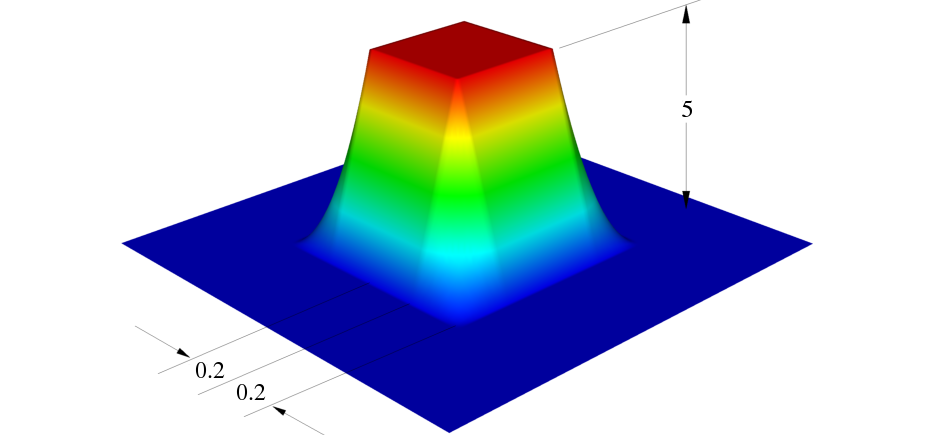
\includegraphics[width=\textwidth]{figures/bio_concentric_rings/u0_schematic}
    \caption{Initial bacteria concentration for the concentric ring problem\label{fig:u0_concentric_rings}}
  \end{center}
\end{figure}
In particular, the linear decay of initial bacteria concentration specified by Equation~\eqref{eq:u0_2_concentric_rings} is chosen because it can be represented exactly with the bilinear and biquadratic elements for the full range of mesh resolutions used in this study.
Also, by fixing the slope of the decay for all mesh resolutions, initial transients caused by inconsistent initial conditions are avoided.  Numerical experiments have shown that failing to maintain consistent initial conditions for reactive transport applications can yield markedly different dynamics in the system. 

\subsubsection{System Parameters}
The relevant parameters for this case were taken from Woodward et~al.~\cite{spatio_temporal_patterns} and are listed in Table~\ref{table:concentric_rings_parameters}.% Parameter values - biological problem no. 1:  concentric rings
\begin{table}[hbtp]
  \begin{center}
    \caption[Nondimensional parameter values for concentric rings]{Nondimensional parameter values for concentric rings (from Woodward et~al.~\cite{spatio_temporal_patterns})}
    \label{table:concentric_rings_parameters}
    \vspace{1em}
    \begin{tabular}{cccccccc} \hline \hline
      $\bv{d_u}$ & $\bv{d_w}$ & $\bv{\alpha}$ & $\bv{\beta}$ & $\bv{\delta}$ & $\bv{\rho}$ & $\bv{\mu}$ & $\bv{\kappa}$ \\
      \unitfrac{1}{4}       & 1          &  7            & 10           & 10            & \unitfrac{1}{10}         & 250         & 0             \\ \hline
    \end{tabular}
  \end{center}
\end{table}
The particular choice $\alpha=7$ de-emphasizes the influence of chemotaxis in comparison to problems considered subsequently.  Put another way, this problem is more sensitive to transport via reaction and diffusion than chemotaxis. For this choice of parameters equations~\eqref{eq:pde_bio_u}--\eqref{eq:pde_bio_w} become
% Bacterial chemotaxis: concentric rings problem, 1st simplification
\begin{align}
  \label{eq:pde_bio_u_concentric_rings_1}
  \frac{\partial u}{\partial t} & = \frac{1}{4} \Delta u - 7 \; \grad{}\cdot \left[ \frac{u}{(1+ v)^2} \grad{v} \right]
                                    + \frac{u}{10} \left( \frac{10 \; w^2}{1 + w^2} - u \right) \\
  \label{eq:pde_bio_v_concentric_rings_1}
  \frac{\partial v}{\partial t} & = \;\;\Delta v + \frac{10 \; w u^2}{250 + u^2} - uv \\
  \label{eq:pde_bio_w_concentric_rings_1}
  \frac{\partial w}{\partial t} & = \;\;\Delta w 
\end{align}
In particular, the parameter $\kappa=0$ decouples the stimulant concentration ($w$) from the bacterial ($u$) and chemoattractant ($v$) concentrations. The physical interpretation of this scenario is that the stimulant supply is essentially unlimited, and its distribution is influenced only though diffusion.  Specifically, the bacteria cannot deplete the stimulant source, no matter how densely populated a region may be.  Additionally, since the stimulant is uniformly distributed initially, even diffusion will be absent for this particular case.  In this scenario the stimulant distribution is completely defined by its initial value, and the governing equations reduce to
% Bacterial chemotaxis: concentric rings problem, 2nd simplification
\begin{align}
  \label{eq:pde_bio_w_concentric_rings_2}
  w &= 5 \\
  \label{eq:pde_bio_u_concentric_rings_2}
  \frac{\partial u}{\partial t} & = \frac{1}{4} \Delta u - 7 \; \grad{}\cdot \left[ \frac{u}{(1+ v)^2} \grad{v} \right]
                                    + u \left( \frac{25}{26} - \frac{u}{10} \right) \\
  \label{eq:pde_bio_v_concentric_rings_2}
  \frac{\partial v}{\partial t} & = \;\;\Delta v + \frac{50 \; u^2}{250 + u^2} - uv
\end{align}
It is worth noting that the decoupling of the governing equations when $\kappa=0$ could be exploited numerically.  In this case the system Jacobian required in the nonlinear solution scheme is smaller than the general case because $\partial R_u/\partial w$, $\partial R_v/\partial w$, $\partial R_w/\partial u$, and $\partial R_w/\partial v$ are identically zero, hence no storage needs to be allocated for these terms.

\subsubsection{Results}
For the parameter set considered in this problem (see Table~\ref{table:concentric_rings_parameters}), the system forms a pattern of concentric rings which grow in number as a function of time until the domain is filled. Figure~\ref{fig:bio_concentric_rings_bacteria} shows a time sequence of bacterial concentration.  The chemoattractant concentration for the same points in time is shown in Figure~\ref{fig:bio_concentric_rings_chemoattractant}. This concentric ring pattern is similar to the top left experimental image shown in Figure~\ref{fig:ecoli_patterns_nature}.
\begin{figure}
  \begin{center}
    \subfigure[t=15.0]{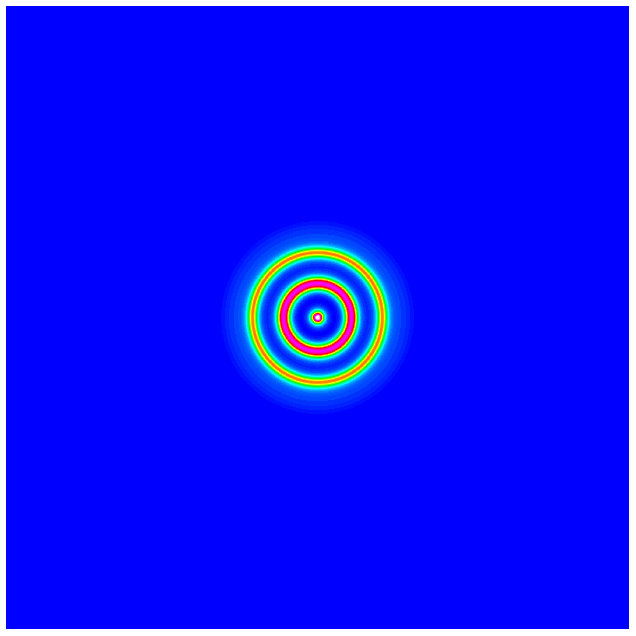
\includegraphics[height=.25\textheight]{figures/bio_concentric_rings/u_00012}}
    \subfigure[t=17.5]{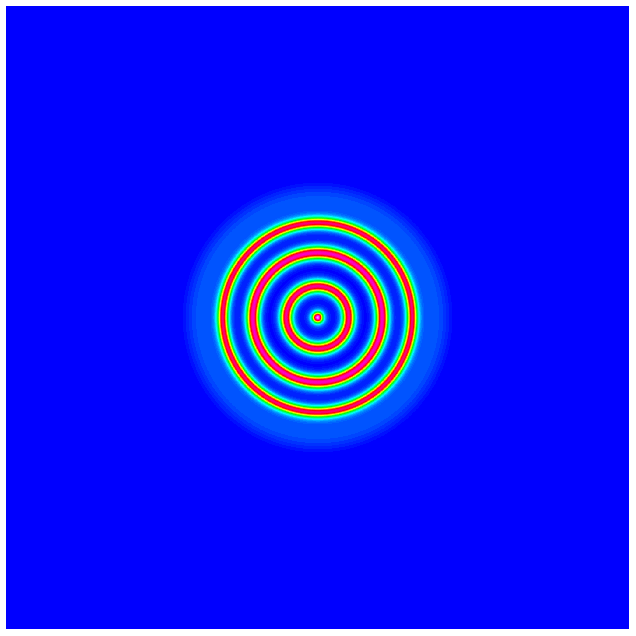
\includegraphics[height=.25\textheight]{figures/bio_concentric_rings/u_00014}} \\
    \subfigure[t=20.0]{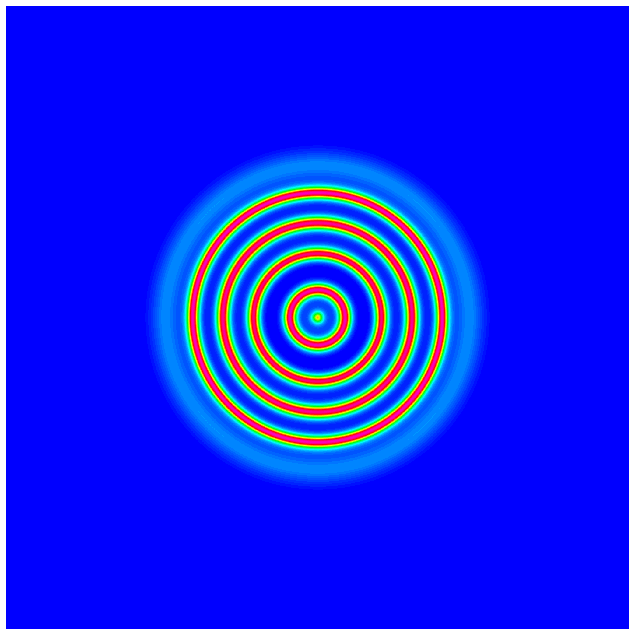
\includegraphics[height=.25\textheight]{figures/bio_concentric_rings/u_00016}}
    \subfigure[t=22.5]{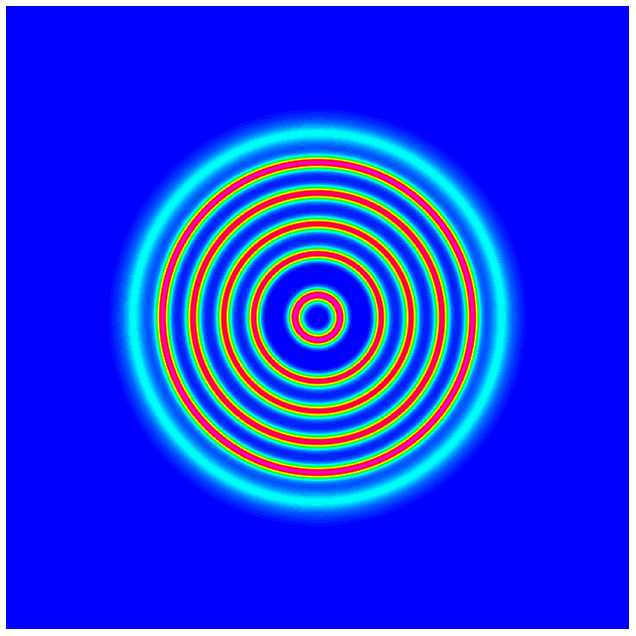
\includegraphics[height=.25\textheight]{figures/bio_concentric_rings/u_00018}} \\
    \subfigure[t=25.0]{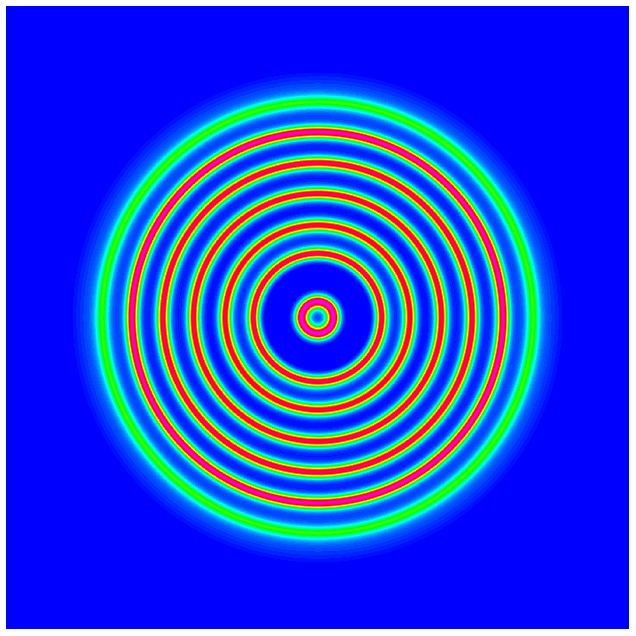
\includegraphics[height=.25\textheight]{figures/bio_concentric_rings/u_00020}}
    \subfigure[t=27.5\label{fig:bio_concentric_rings_bacteria_t27.5}]{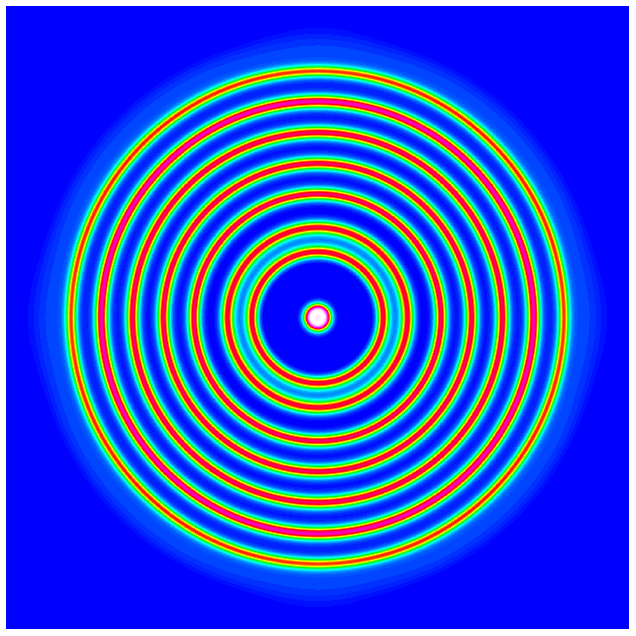
\includegraphics[height=.25\textheight]{figures/bio_concentric_rings/u_00022}}
    \caption{Continuous concentric advancing rings. Bacteria concentration history.\label{fig:bio_concentric_rings_bacteria}}
  \end{center}
\end{figure}

\begin{figure}
  \begin{center}
    \subfigure[t=15.0]{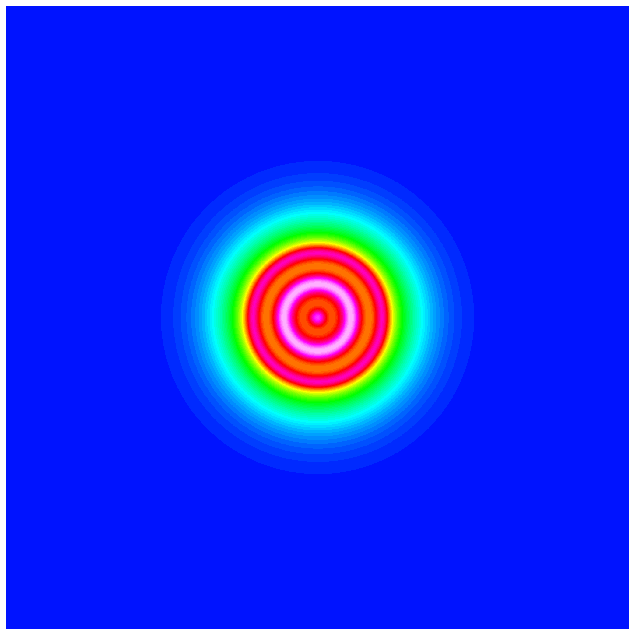
\includegraphics[height=.25\textheight]{figures/bio_concentric_rings/v_00012}}
    \subfigure[t=17.5]{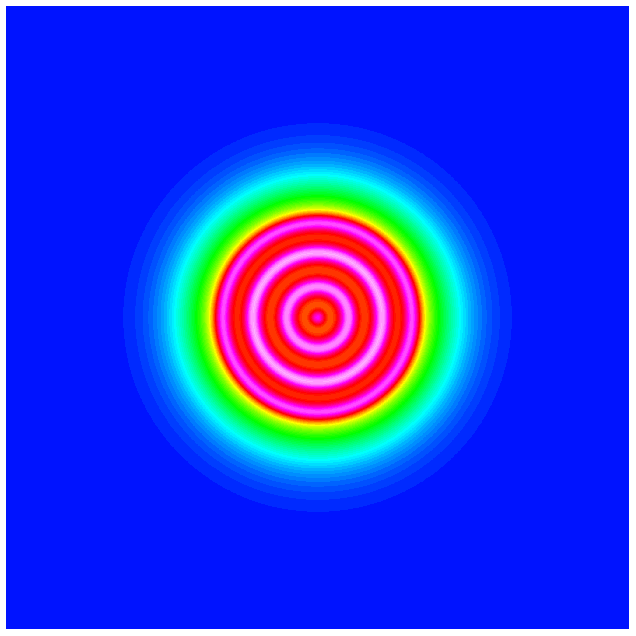
\includegraphics[height=.25\textheight]{figures/bio_concentric_rings/v_00014}} \\
    \subfigure[t=20.0]{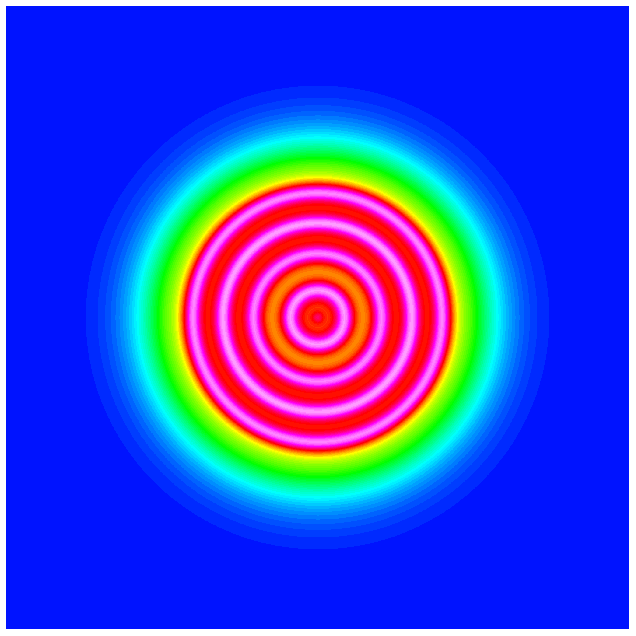
\includegraphics[height=.25\textheight]{figures/bio_concentric_rings/v_00016}}
    \subfigure[t=22.5]{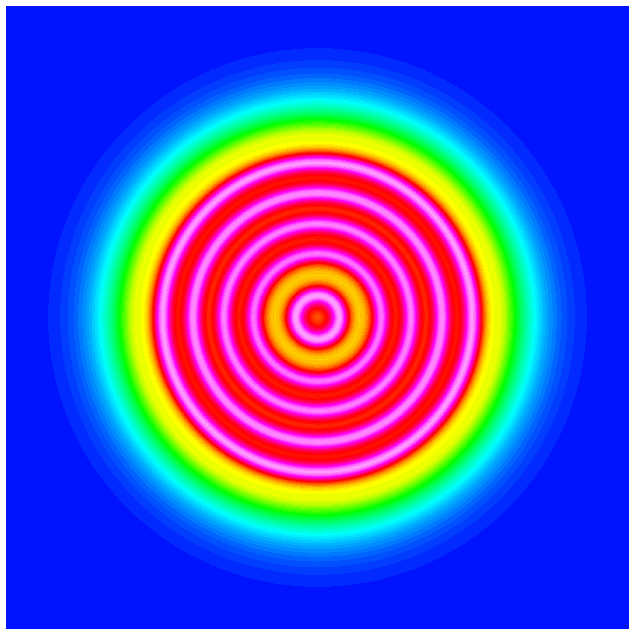
\includegraphics[height=.25\textheight]{figures/bio_concentric_rings/v_00018}} \\
    \subfigure[t=25.0]{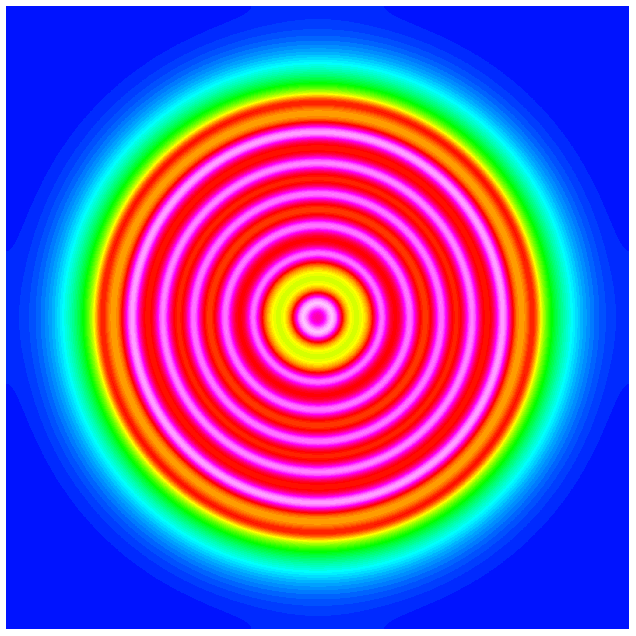
\includegraphics[height=.25\textheight]{figures/bio_concentric_rings/v_00020}}
    \subfigure[t=27.5\label{fig:bio_concentric_rings_chemoattractant_t27.5}]{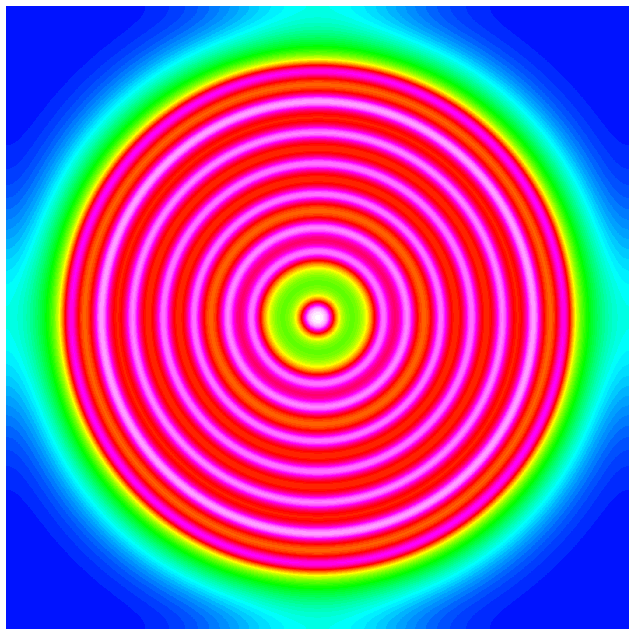
\includegraphics[height=.25\textheight]{figures/bio_concentric_rings/v_00022}}
    \caption{Continuous concentric advancing rings. Chemoattractant concentration history.\label{fig:bio_concentric_rings_chemoattractant}}
  \end{center}
\end{figure}

It is interesting to note that the spatial pattern shown in the figures exhibits radial symmetry.  It is not immediately obvious that this would be the case, especially given the clearly two-dimensional nature of the initial conditions (c.f. Figure~\ref{fig:u0_concentric_rings}).  Figure~\ref{fig:bio_concentric_rings_startup} details the initial transients for the first nine timesteps in the simulation with a fixed step size $\Delta t=2\times 10^{-3}$.
\begin{figure}
  \begin{center}
    \subfigure[t=0.000]{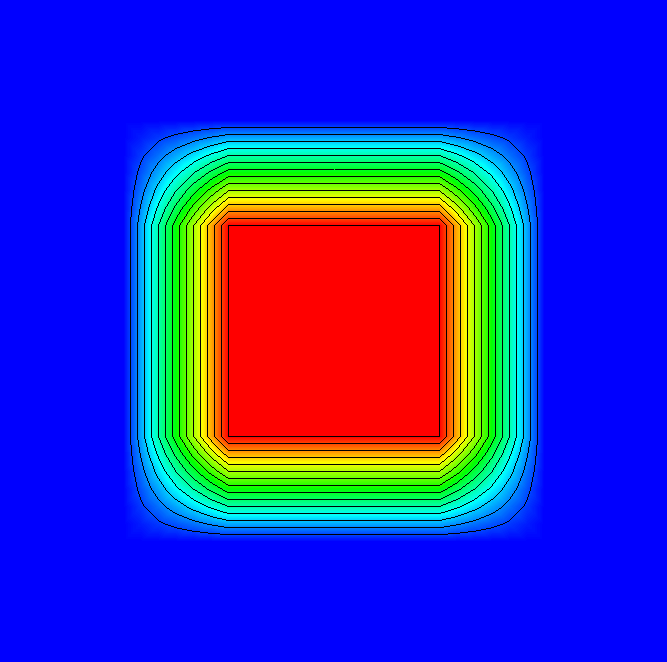
\includegraphics[width=.31\textwidth]{figures/bio_concentric_rings/initial_transient/dt_2e-3/u-rsnapgmv0000}}
    \subfigure[t=0.002]{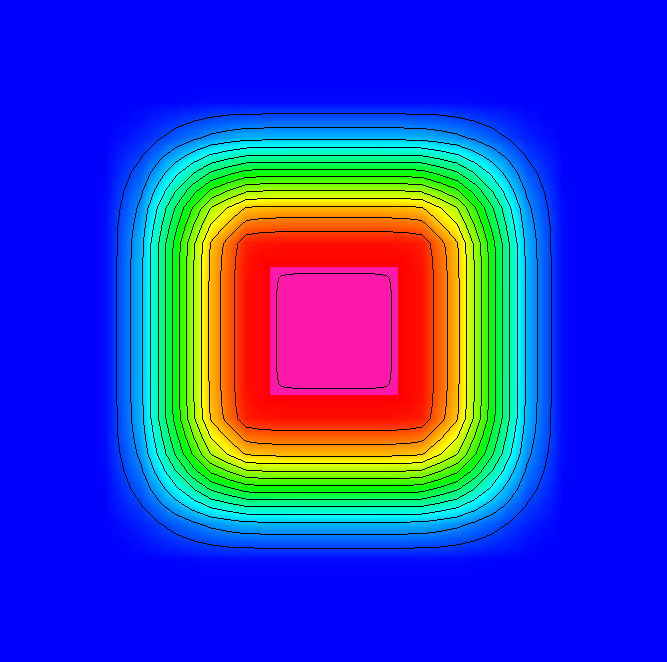
\includegraphics[width=.31\textwidth]{figures/bio_concentric_rings/initial_transient/dt_2e-3/u-rsnapgmv0001}}
    \subfigure[t=0.004]{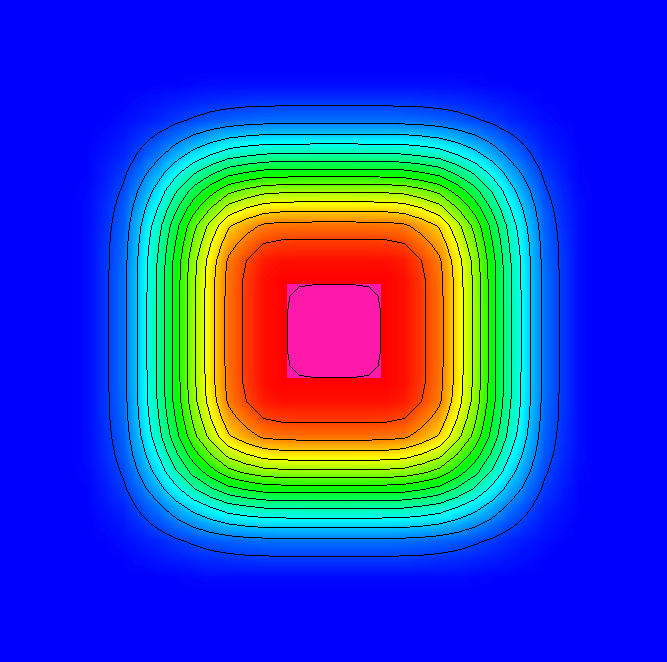
\includegraphics[width=.31\textwidth]{figures/bio_concentric_rings/initial_transient/dt_2e-3/u-rsnapgmv0002}} \\
    \subfigure[t=0.006]{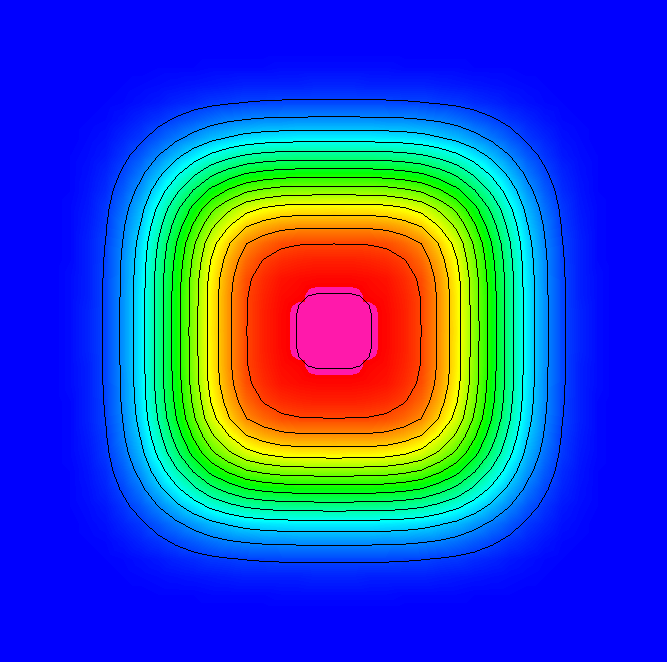
\includegraphics[width=.31\textwidth]{figures/bio_concentric_rings/initial_transient/dt_2e-3/u-rsnapgmv0003}}
    \subfigure[t=0.008]{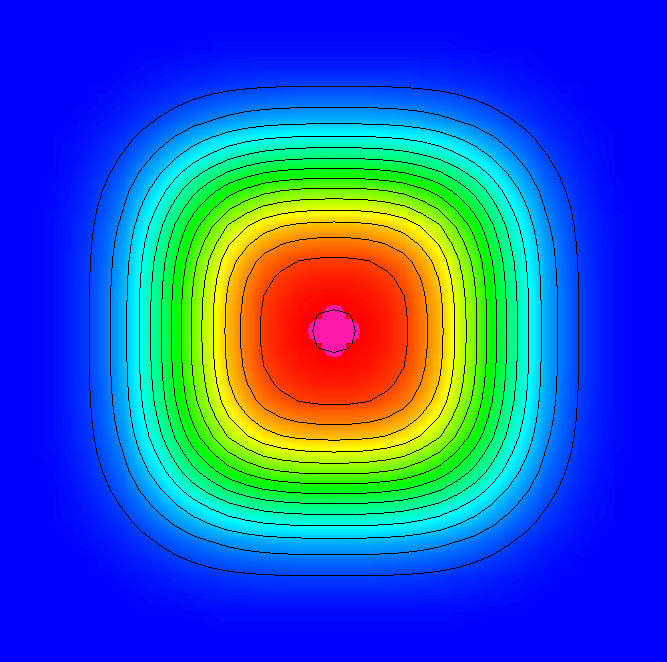
\includegraphics[width=.31\textwidth]{figures/bio_concentric_rings/initial_transient/dt_2e-3/u-rsnapgmv0004}}
    \subfigure[t=0.010]{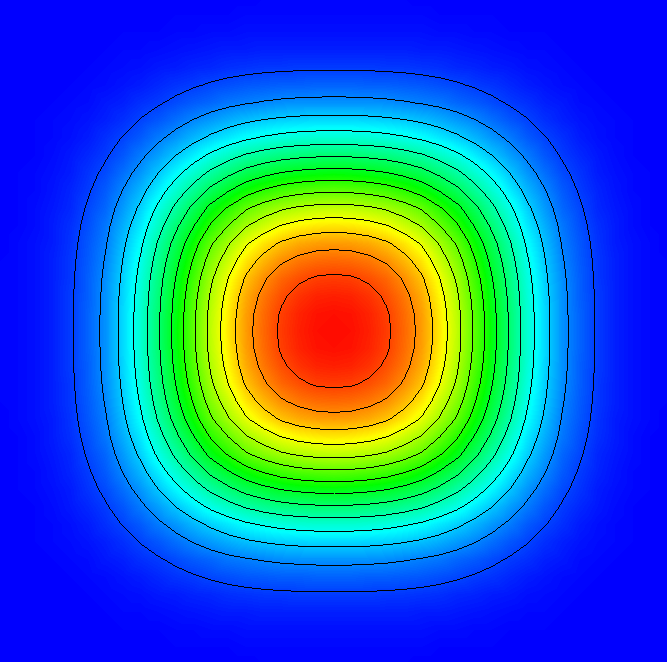
\includegraphics[width=.31\textwidth]{figures/bio_concentric_rings/initial_transient/dt_2e-3/u-rsnapgmv0005}} \\
    \subfigure[t=0.006]{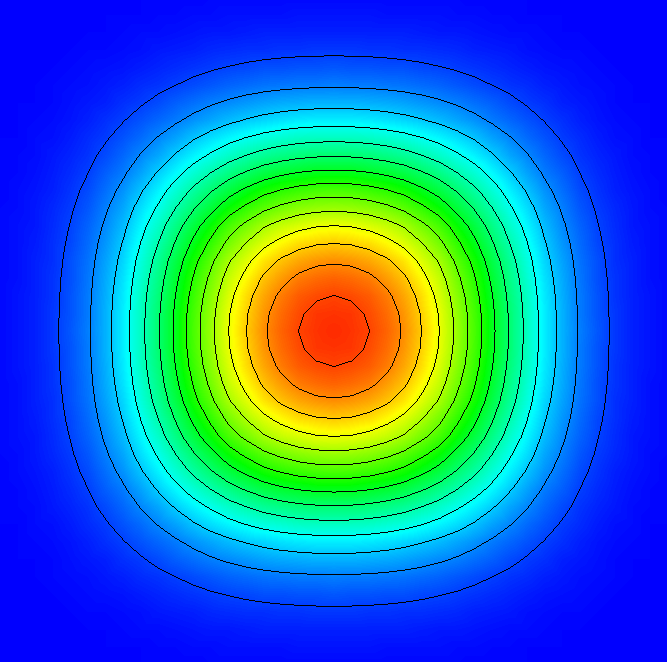
\includegraphics[width=.31\textwidth]{figures/bio_concentric_rings/initial_transient/dt_2e-3/u-rsnapgmv0006}}
    \subfigure[t=0.008]{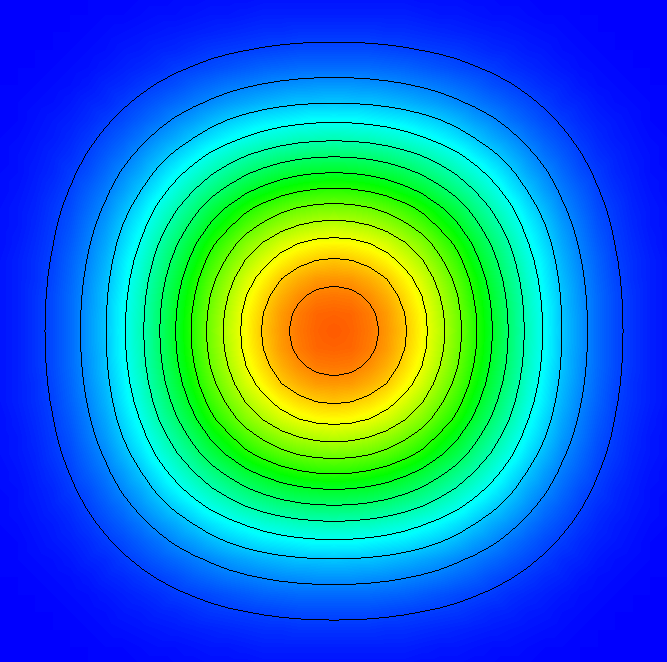
\includegraphics[width=.31\textwidth]{figures/bio_concentric_rings/initial_transient/dt_2e-3/u-rsnapgmv0007}}
    \subfigure[t=0.010]{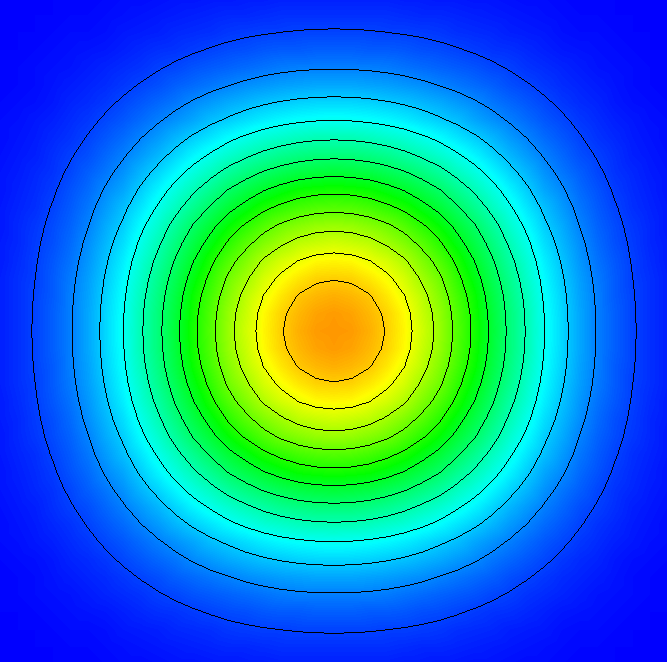
\includegraphics[width=.31\textwidth]{figures/bio_concentric_rings/initial_transient/dt_2e-3/u-rsnapgmv0008}}
    \caption[Initial transient and smoothing of the initial bacteria concentration.]{Initial transient and smoothing of the initial bacteria concentration.  A $[-1,1]^2$ subregion of the mesh is shown with linear contours ranging from $[0,5]$.\label{fig:bio_concentric_rings_startup}}
  \end{center}
\end{figure}
It is clear from the figure that the initial, tensor-product profile is quickly diffused.  The corner regions of maximum gradient are smoothed quickly and then the entire profile begins to expand and becomes symmetric.  After nine timesteps the asymmetry  of the initial conditions is virtually eliminated.  Based on this behavior, it is clear that the initial transients are diffusion dominated.  The isotropic diffusion essentially smooths the initial conditions into a radially symmetric profile before significant reaction and chemotaxis begin.  It should be possible to exploit this radial symmetry for a significant computational savings.  By reformulating \eqref{eq:pde_bio_u}--\eqref{eq:pde_bio_w} in terms of polar $(r,\theta)$ coordinates and assuming $\theta$-symmetry the spatial dimensionality of the system is reduced.  Thus it should be possible to solve a reduced one-dimensional problem for the subset of parameters which yield radially symmetric patterns.

%The number of rings grows in time, but the relative width of each ring is essentially constant.  This is in some sense similar to tree rings.  The number of rings in a tree is dependent upon the age of the tree, while the width of individual rings is dependent on environmental factors during the year the ring is formed.  Relatively thicker rings within a tree indicate healthier years, which is often correlated to increased rainfall.  For this case the parameter $\kappa=0$ decouples the stimulant (food) concentration from the proliferation of bacteria, hence the stimulant supply is essentially unlimited.  Thus, the developing spatial pattern has no time dependence on the stimulant concentration.  It would be interesting to repeat this experiment with $\kappa\ne 0$ to determine if the tree ring analogy holds in the case of variable stimulant.

The maximum nondimensional bacteria and chemoattractant concentrations for this parameter set are plotted as a function of time for a series of hierarchically refined meshes in Figure~\ref{fig:bio_concentric_rings_max_history}.
\begin{figure}[hbp]
  \begin{center}
    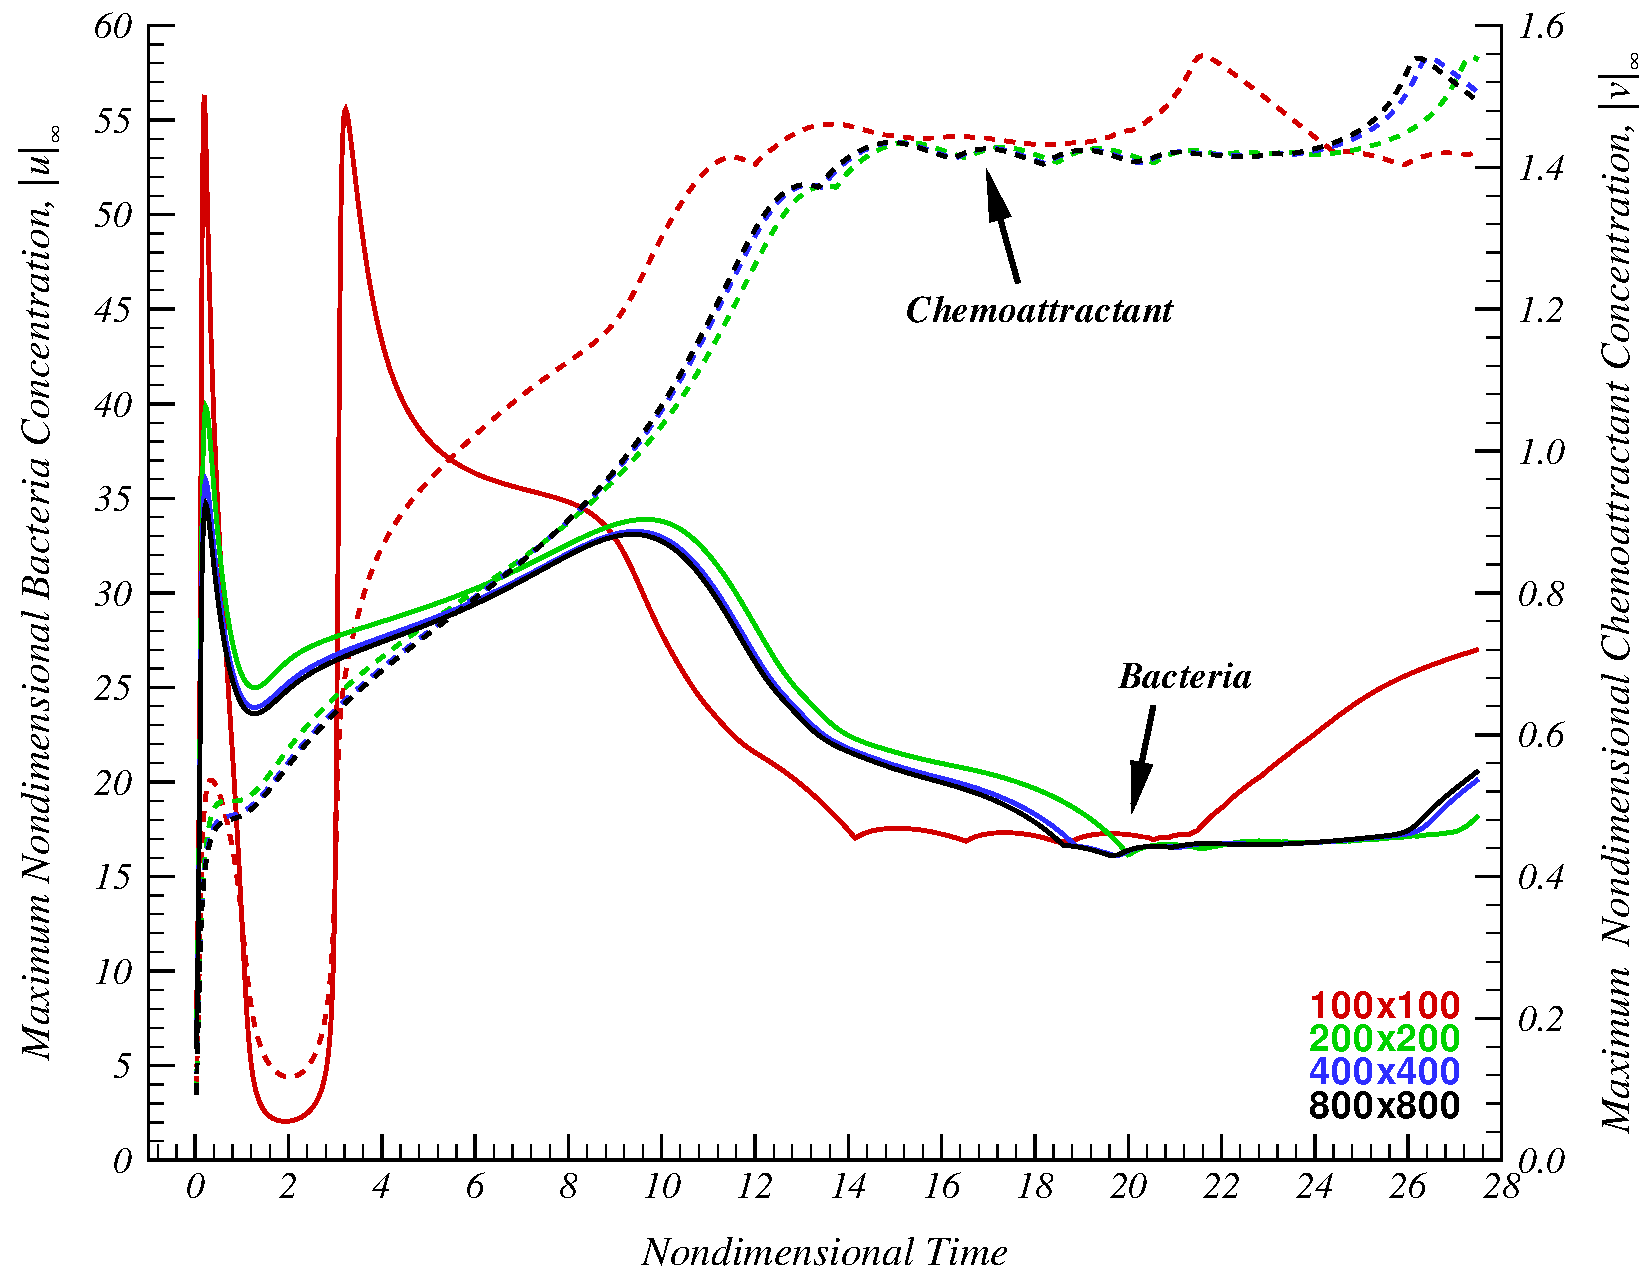
\includegraphics[width=\textwidth]{figures/bio_concentric_rings/max_history}
    \caption{Continuous concentric advancing rings. Maximum bacteria and chemoattractant history for a sequence of meshes composed of biquadratic finite elements.\label{fig:bio_concentric_rings_max_history}}
  \end{center}
\end{figure}
It is evident from the figure that the dynamics captured with the $100 \times 100$ mesh are very inaccurate, while those of the $200 \times 200$,  $400 \times 400$, and $800 \times 800$ meshes essentially agree.  All cases predict a sharp initial increase in bacteria concentration in the first (nondimensional) second of the simulation.  Focusing now on the finer mesh results, the maximum bacteria concentration then drops to a value of $\|u\|_\infty\approx 25$ at around $t=1$ while the maximum chemoattractant concentration steadily increases.  Both then increase until $t\approx 10$.  For this entire time range the system contains only a single ``ring'' located at the origin of the domain.  That is, all the dynamics prior to $t\approx 10$ are directly tied to the initial conditions.

At subsequent times rings begin to form. During this period the maximum value of the chemoattractant is essentially constant at $\approx 1.4$.  Small amplitude oscillations are clearly evident which correspond to the formation of new rings.  The increase in both $\|u\|_\infty$ and $\|v\|_\infty$ at the end of the simulation is attributed to interactions with the boundary of the domain. It can be seen in Figure~\ref{fig:bio_concentric_rings_chemoattractant_t27.5} that in the final portion of the simulation the boundary is indeed affecting the solution, as expected.

  Formally, the error in the solution is defined as
\begin{align}
  e_u & = u_h  - u \label{eq:bio_error_u_exact} \\
  e_v & = v_h  - v \label{eq:bio_error_v_exact} \\
  e_w & = w_h  - w \label{eq:bio_error_w_exact}  
\end{align}
where $()_h$ denotes the approximate solution obtained on a mesh with a characteristic spacing of $h$ and $(u,v,w)$ are the (unknown) exact solution values.  Clearly the exact solution is not known in general.  However, it is possible to approximate~\eqref{eq:bio_error_u_exact}--\eqref{eq:bio_error_w_exact} by comparing the solution on two different meshes, one being very fine.  That is,
\begin{alignat}{2}
  e_u &\approx e^c_u & = &\; u_c  - u_f \label{eq:bio_error_u_approx} \\
  e_v &\approx e^c_v & = &\; v_c  - v_f \label{eq:bio_error_v_approx} \\
  e_w &\approx e^c_w & = &\; w_c  - w_f \label{eq:bio_error_w_approx}  
\end{alignat}
where $()_c$ and $()_f$ denote coarse and fine mesh solution values, respectively. Figures~\ref{fig:bio_concentric_rings_bacteria_error} and~\ref{fig:bio_concentric_rings_chemoattractant_error} use this method to illustrate the error in the $100\times 100$, $200\times 200$, and $400\times 400$ biquadratic finite element meshes via comparison with the $800\times 800$ solution. 

\begin{figure}
  \begin{center}
    \subfigure[t=15.0]{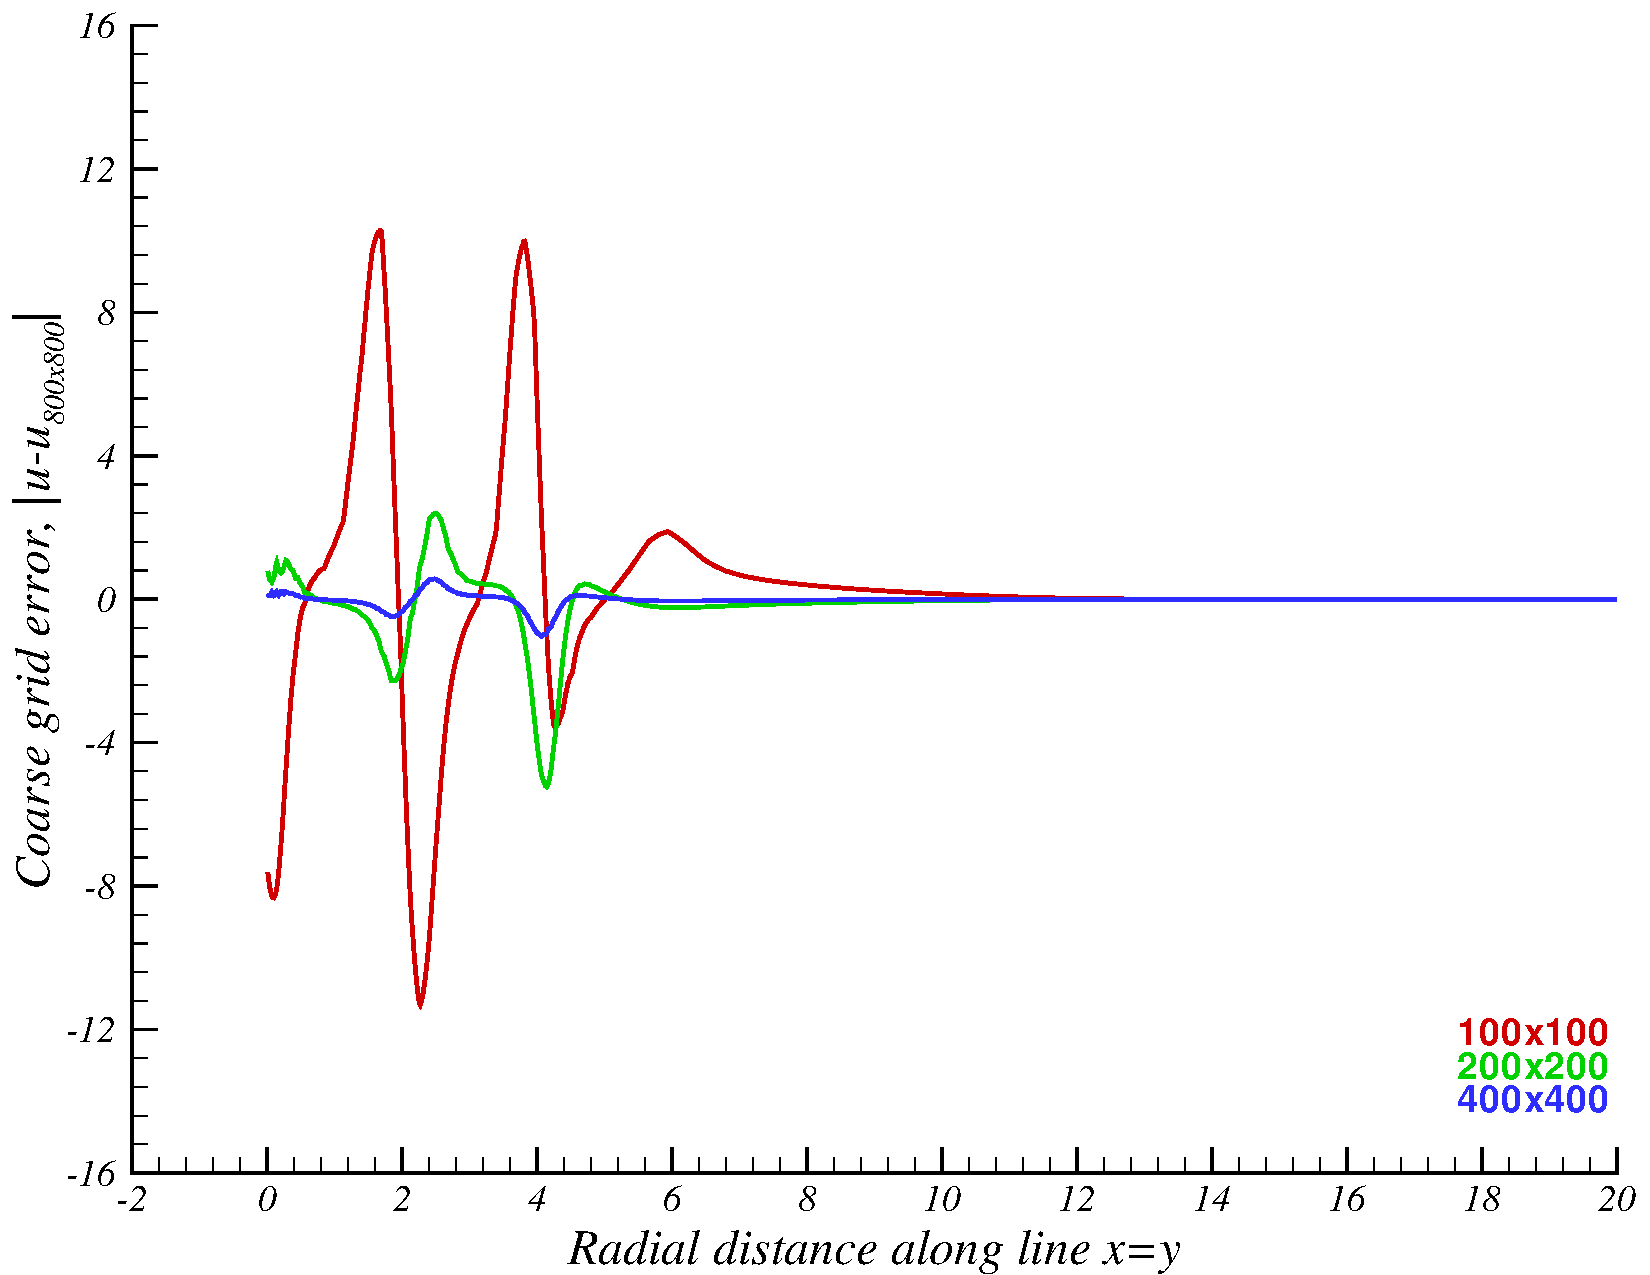
\includegraphics[height=.25\textheight]{figures/bio_concentric_rings/err_u_00012}}
    \subfigure[t=17.5]{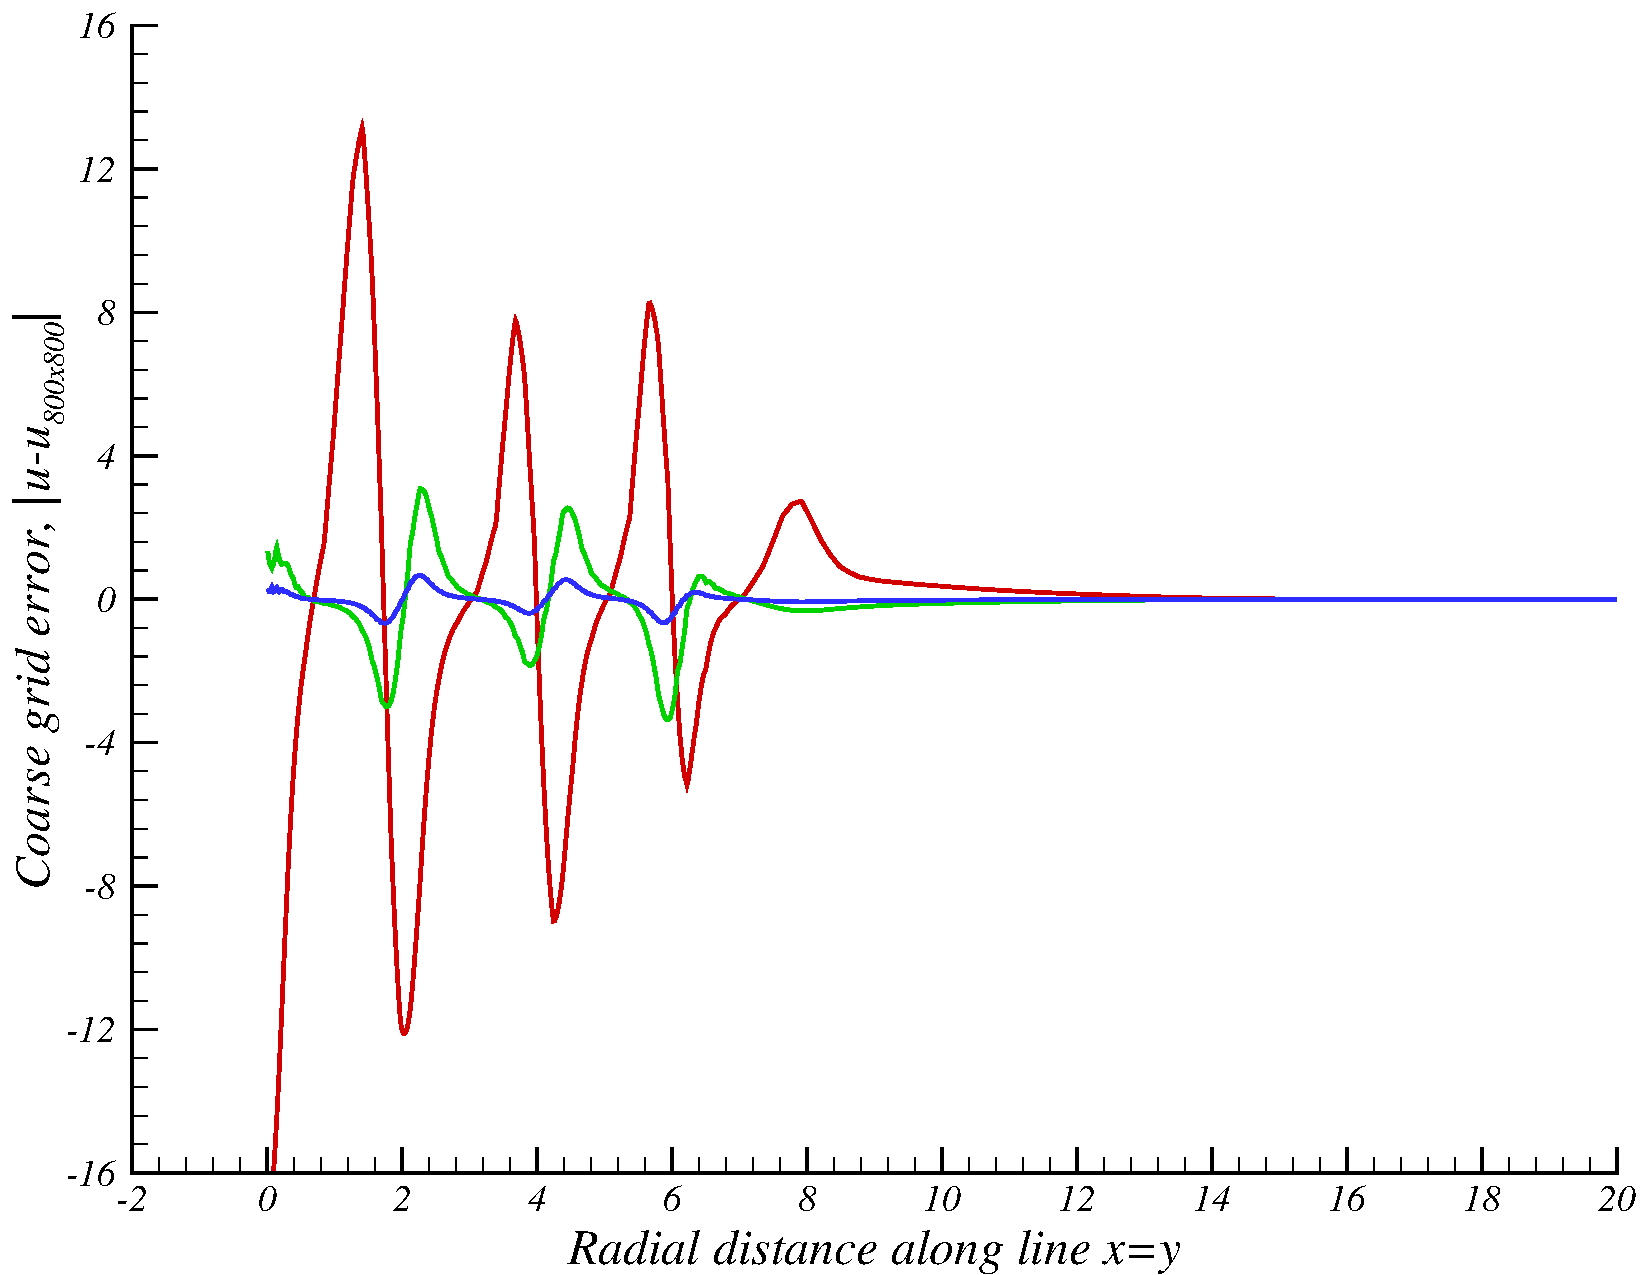
\includegraphics[height=.25\textheight]{figures/bio_concentric_rings/err_u_00014}} \\
    \subfigure[t=20.0]{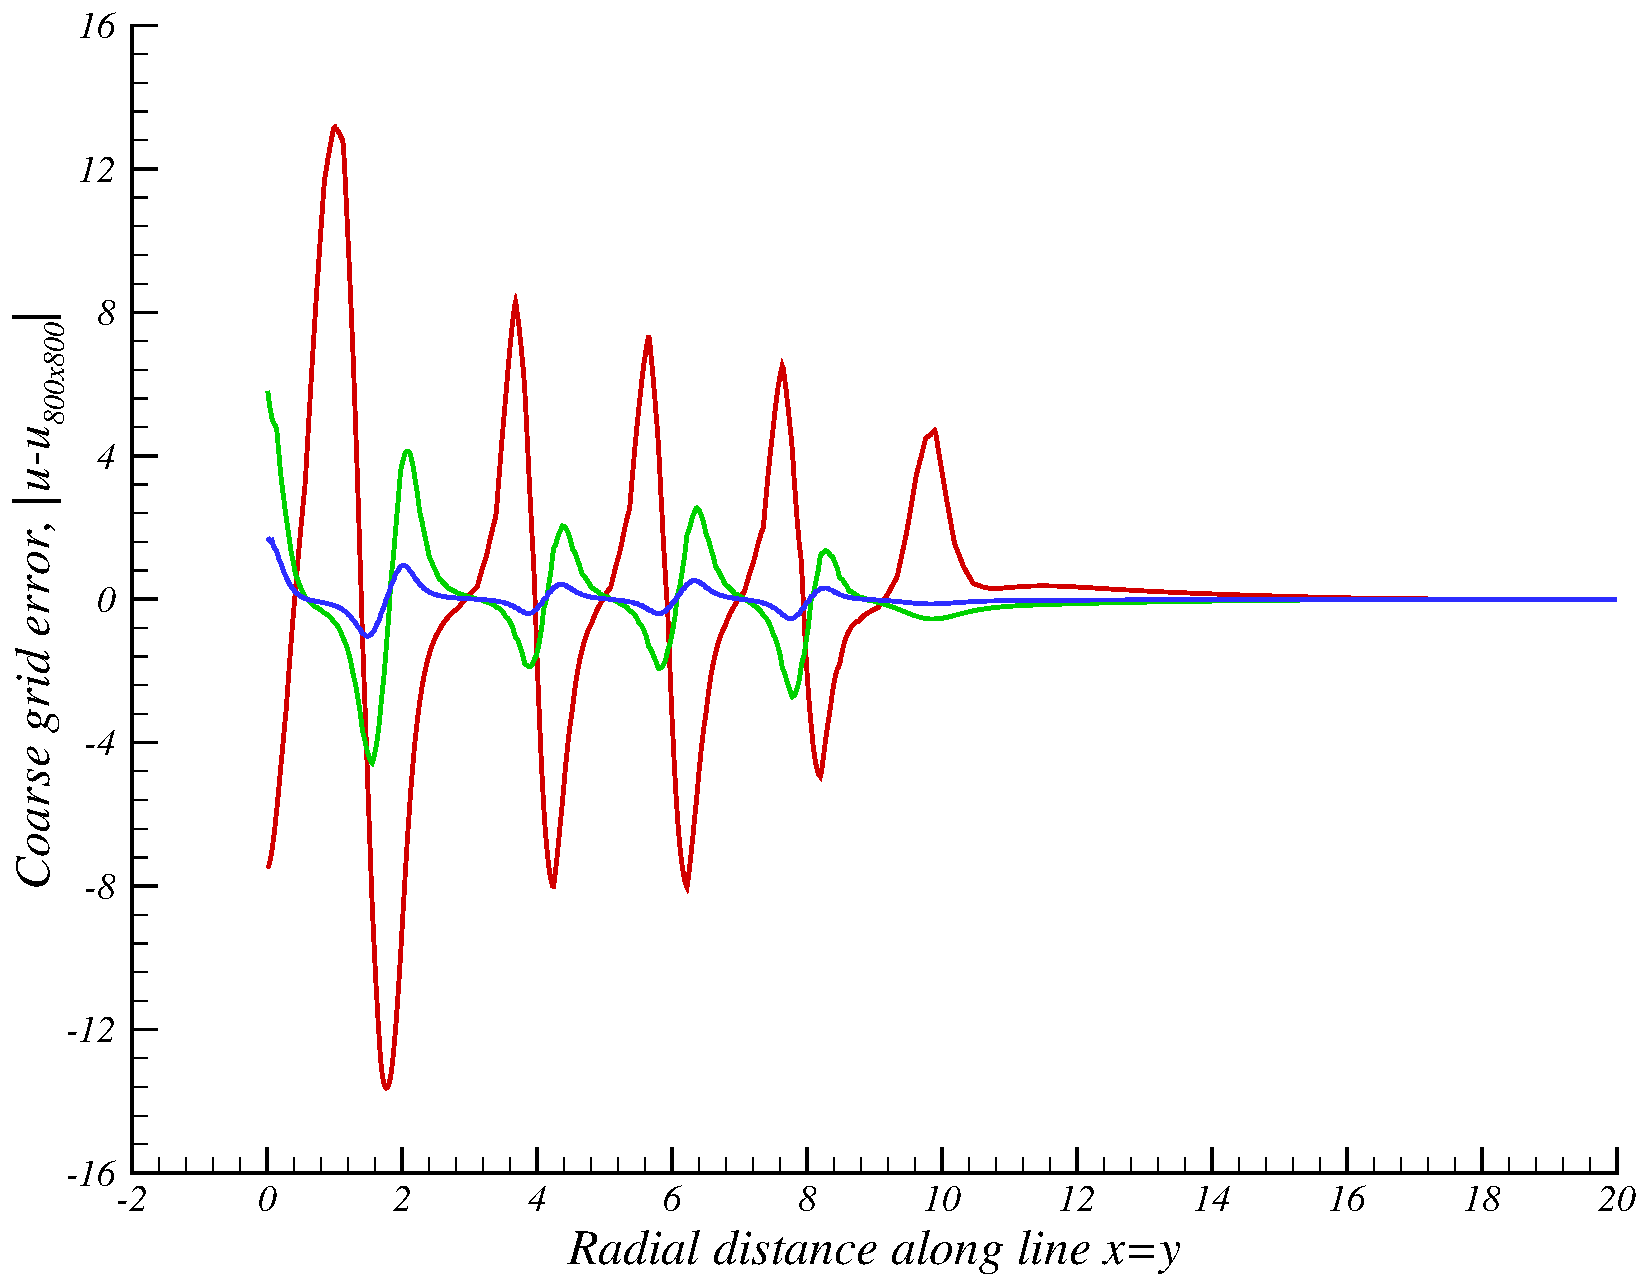
\includegraphics[height=.25\textheight]{figures/bio_concentric_rings/err_u_00016}}
    \subfigure[t=22.5]{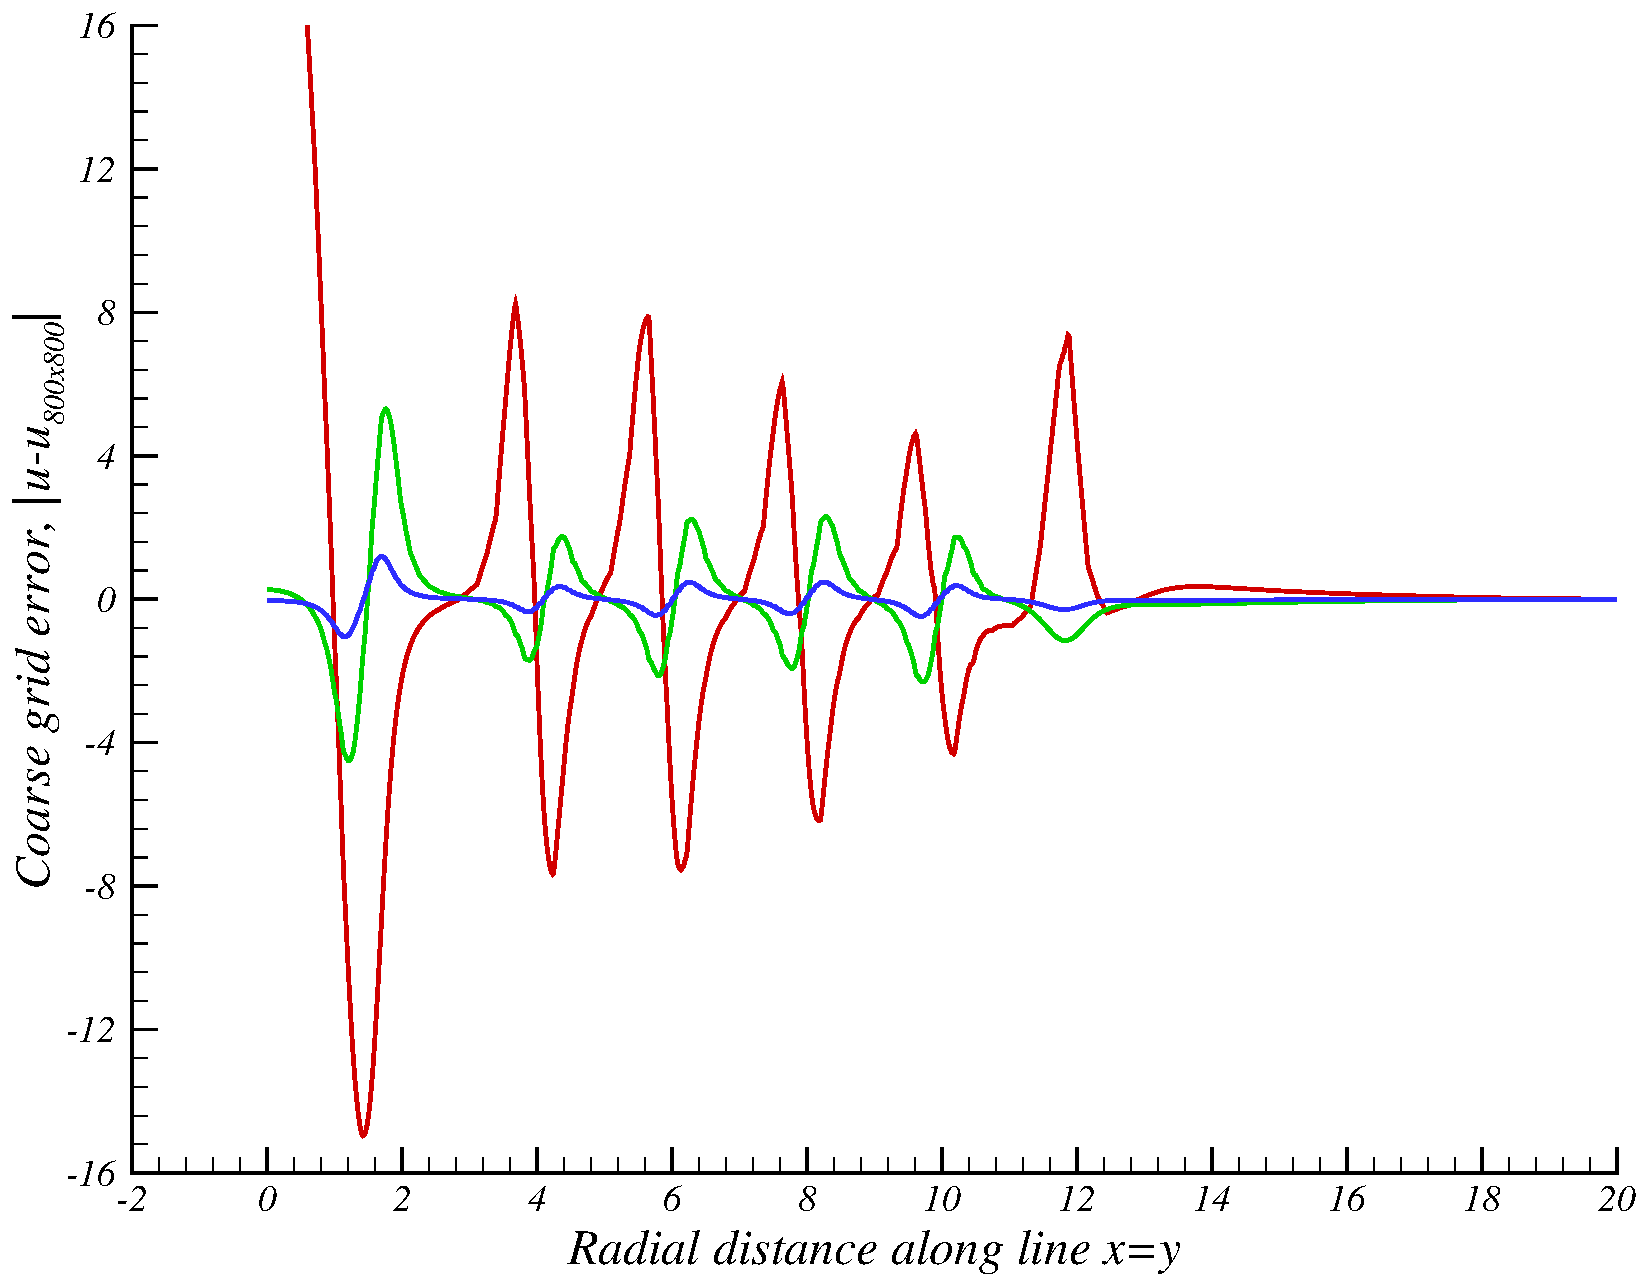
\includegraphics[height=.25\textheight]{figures/bio_concentric_rings/err_u_00018}} \\
    \subfigure[t=25.0]{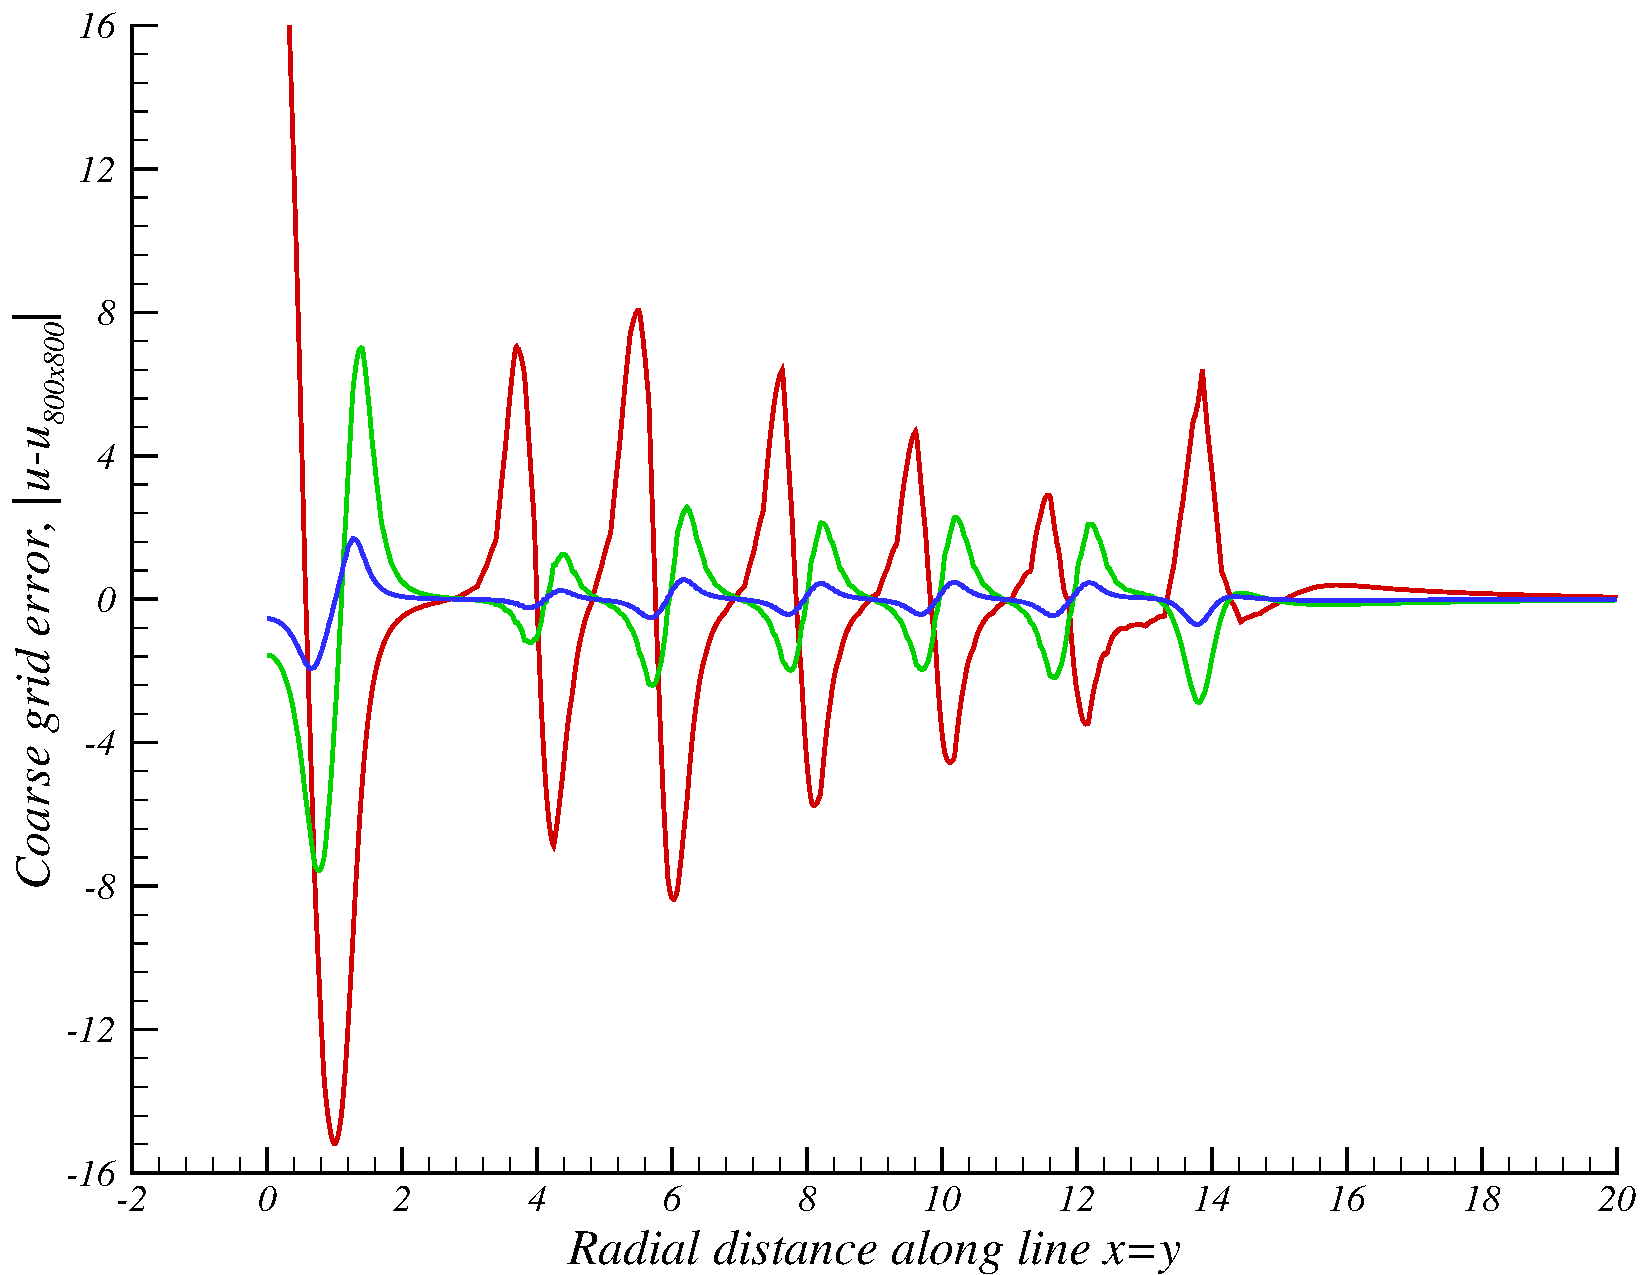
\includegraphics[height=.25\textheight]{figures/bio_concentric_rings/err_u_00020}}
    \subfigure[t=27.5]{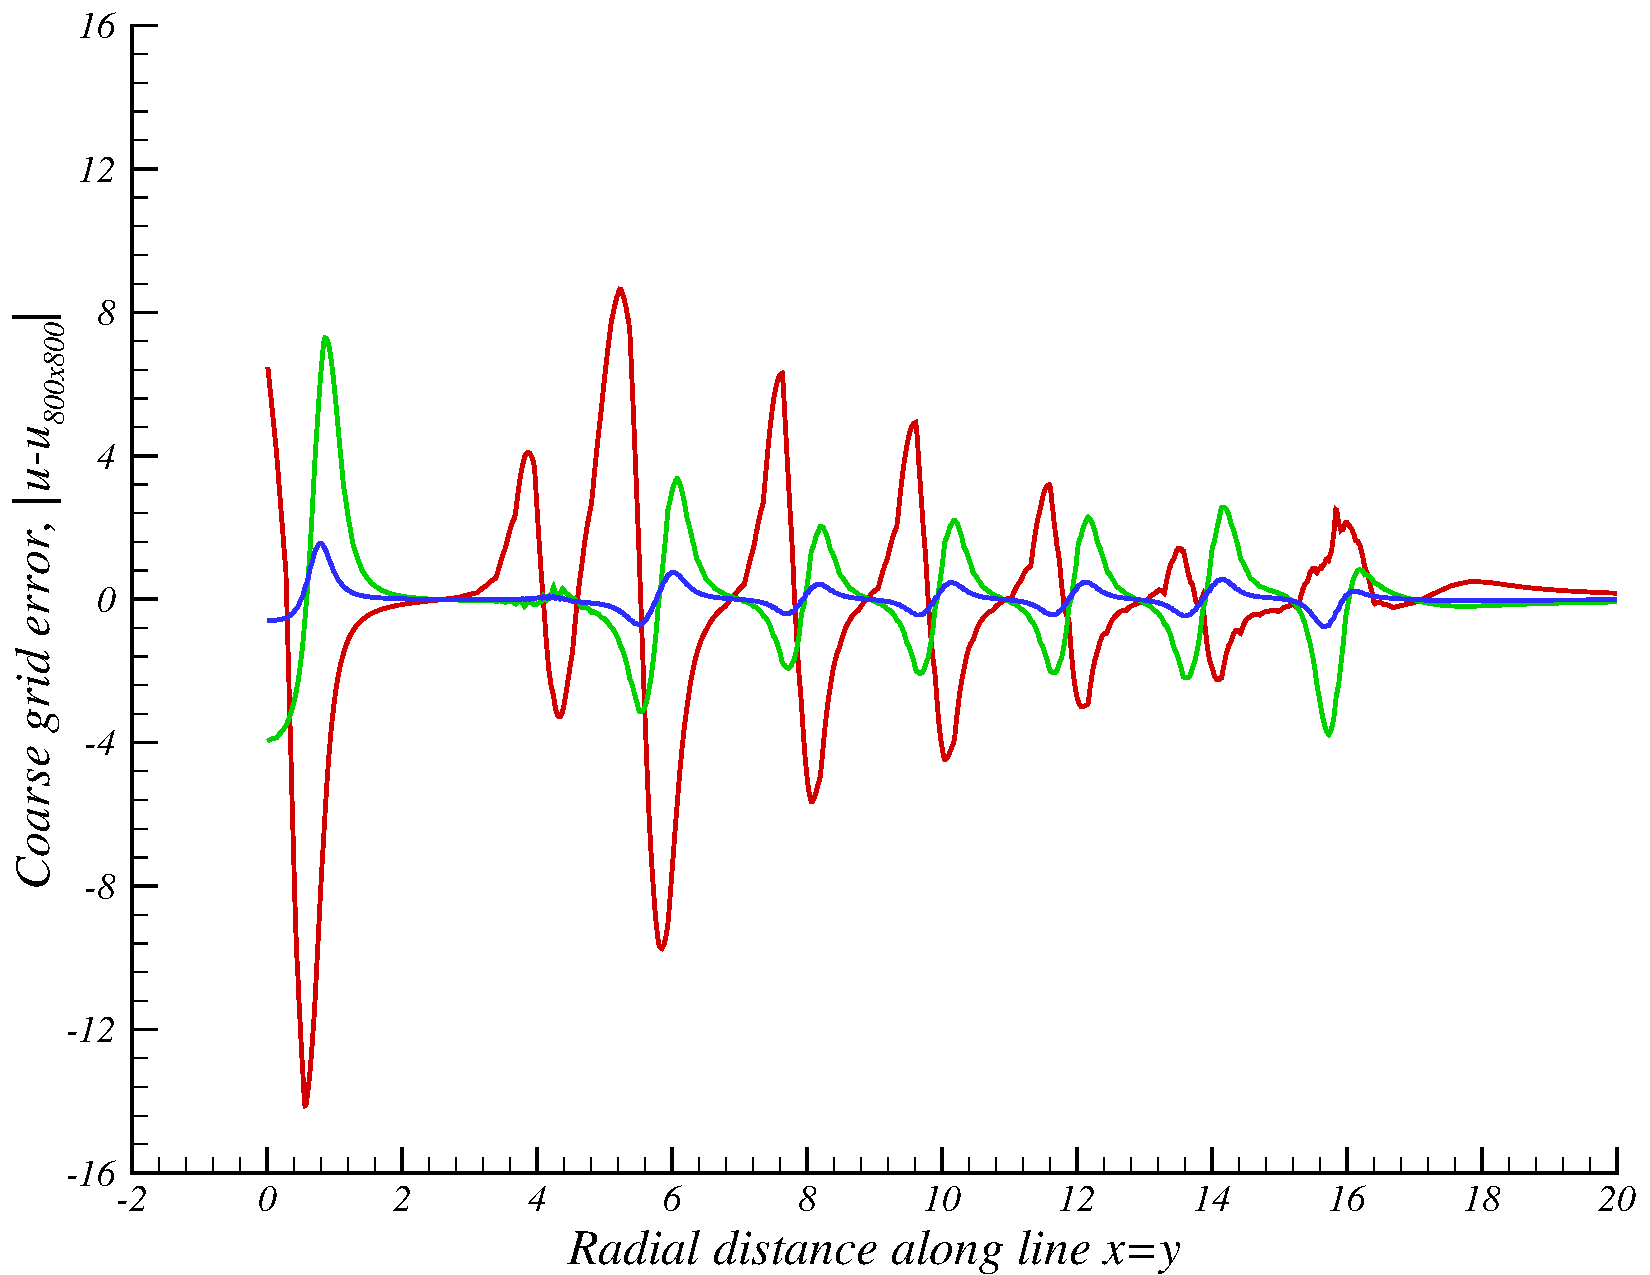
\includegraphics[height=.25\textheight]{figures/bio_concentric_rings/err_u_00022}}
    \caption{Continuous concentric advancing rings. Coarse grid bacteria concentration error history.\label{fig:bio_concentric_rings_bacteria_error}}
  \end{center}
\end{figure}

\begin{figure}
  \begin{center}
    \subfigure[t=15.0]{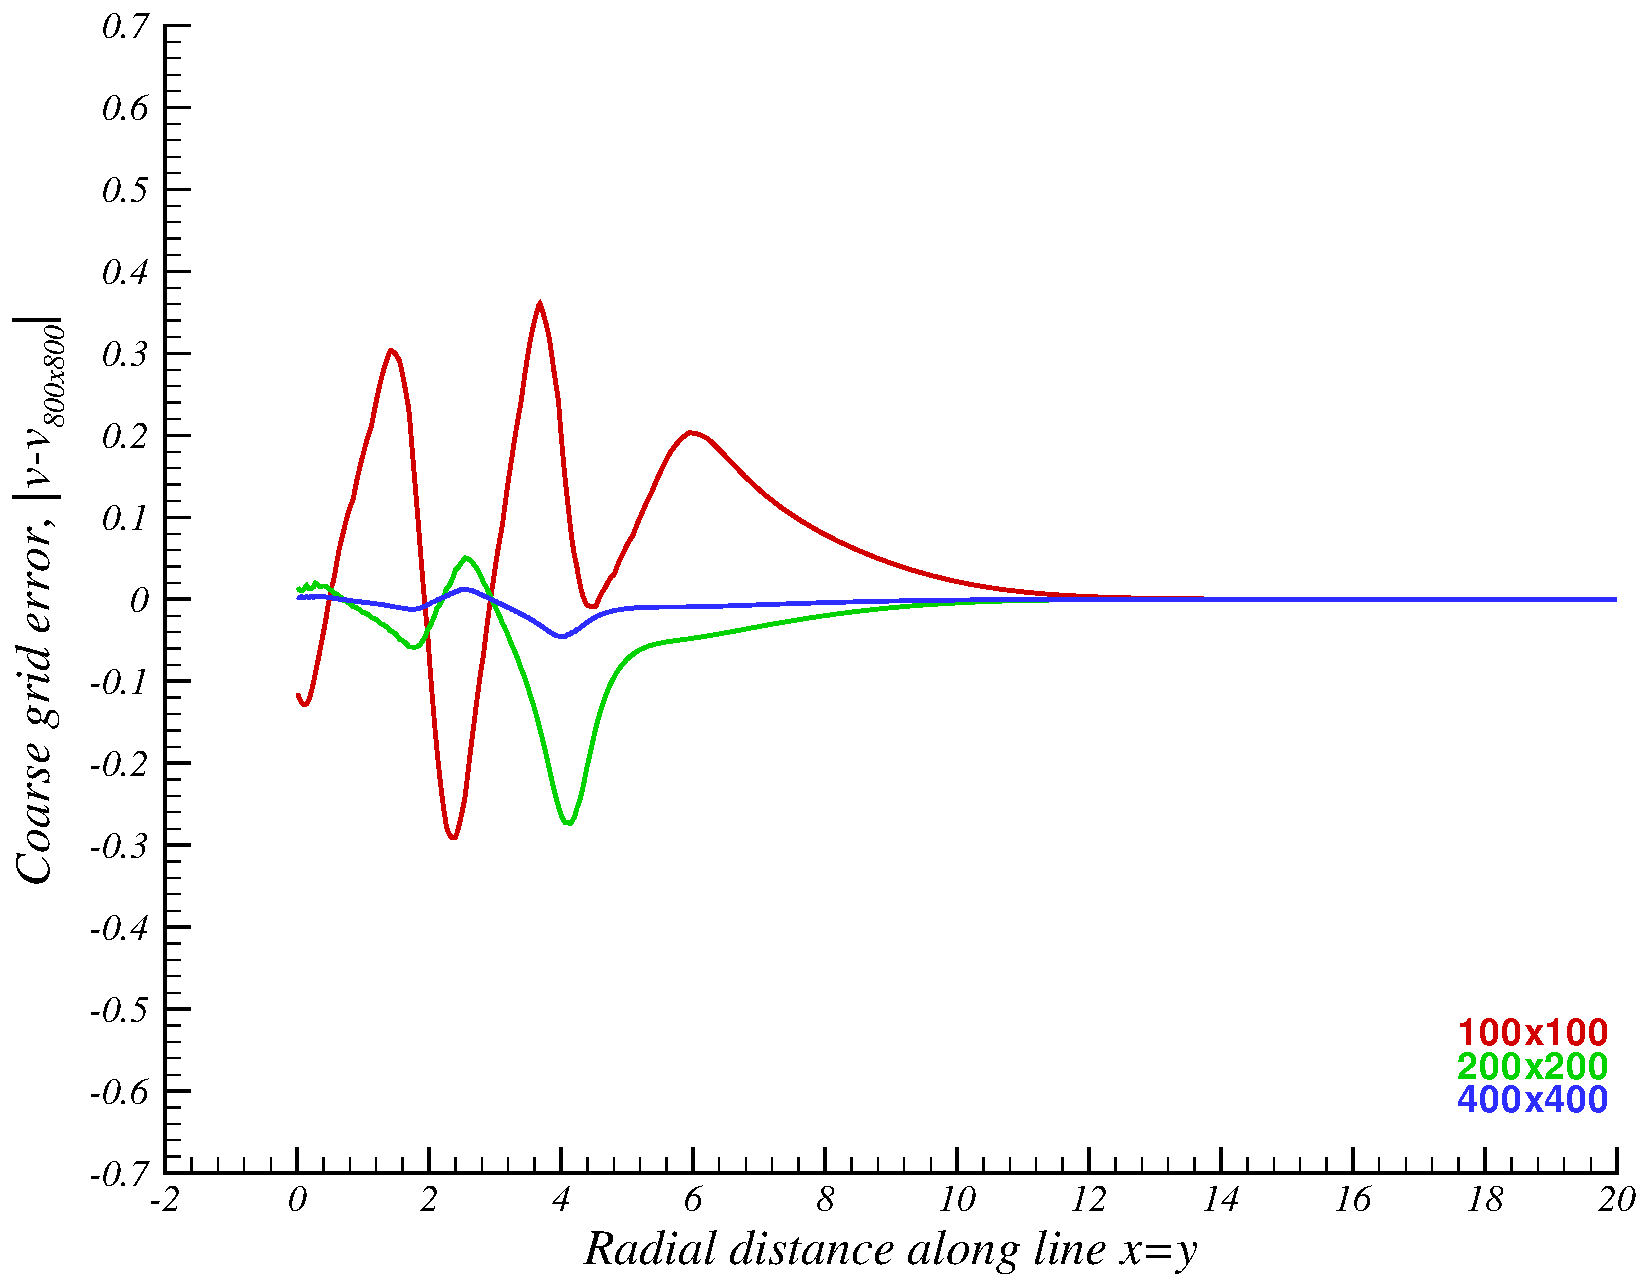
\includegraphics[height=.25\textheight]{figures/bio_concentric_rings/err_v_00012}}
    \subfigure[t=17.5]{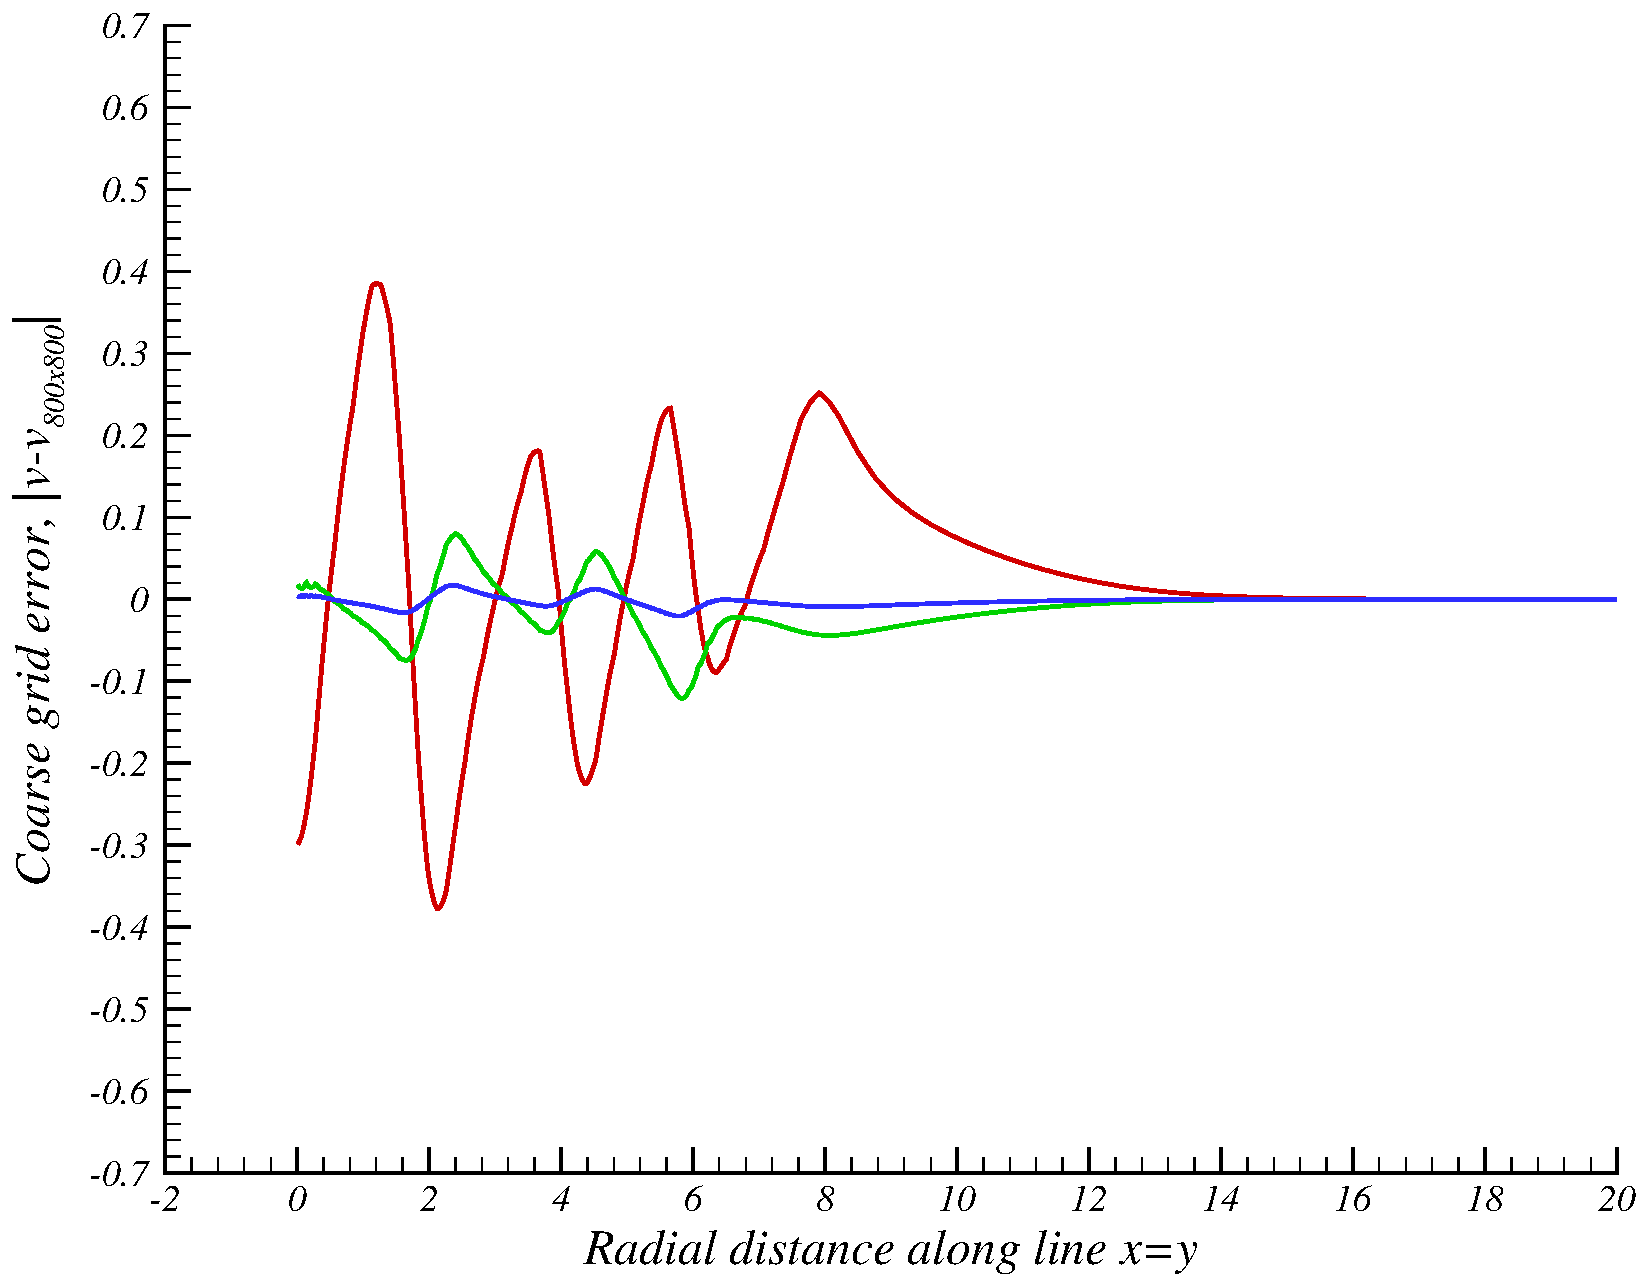
\includegraphics[height=.25\textheight]{figures/bio_concentric_rings/err_v_00014}} \\
    \subfigure[t=20.0]{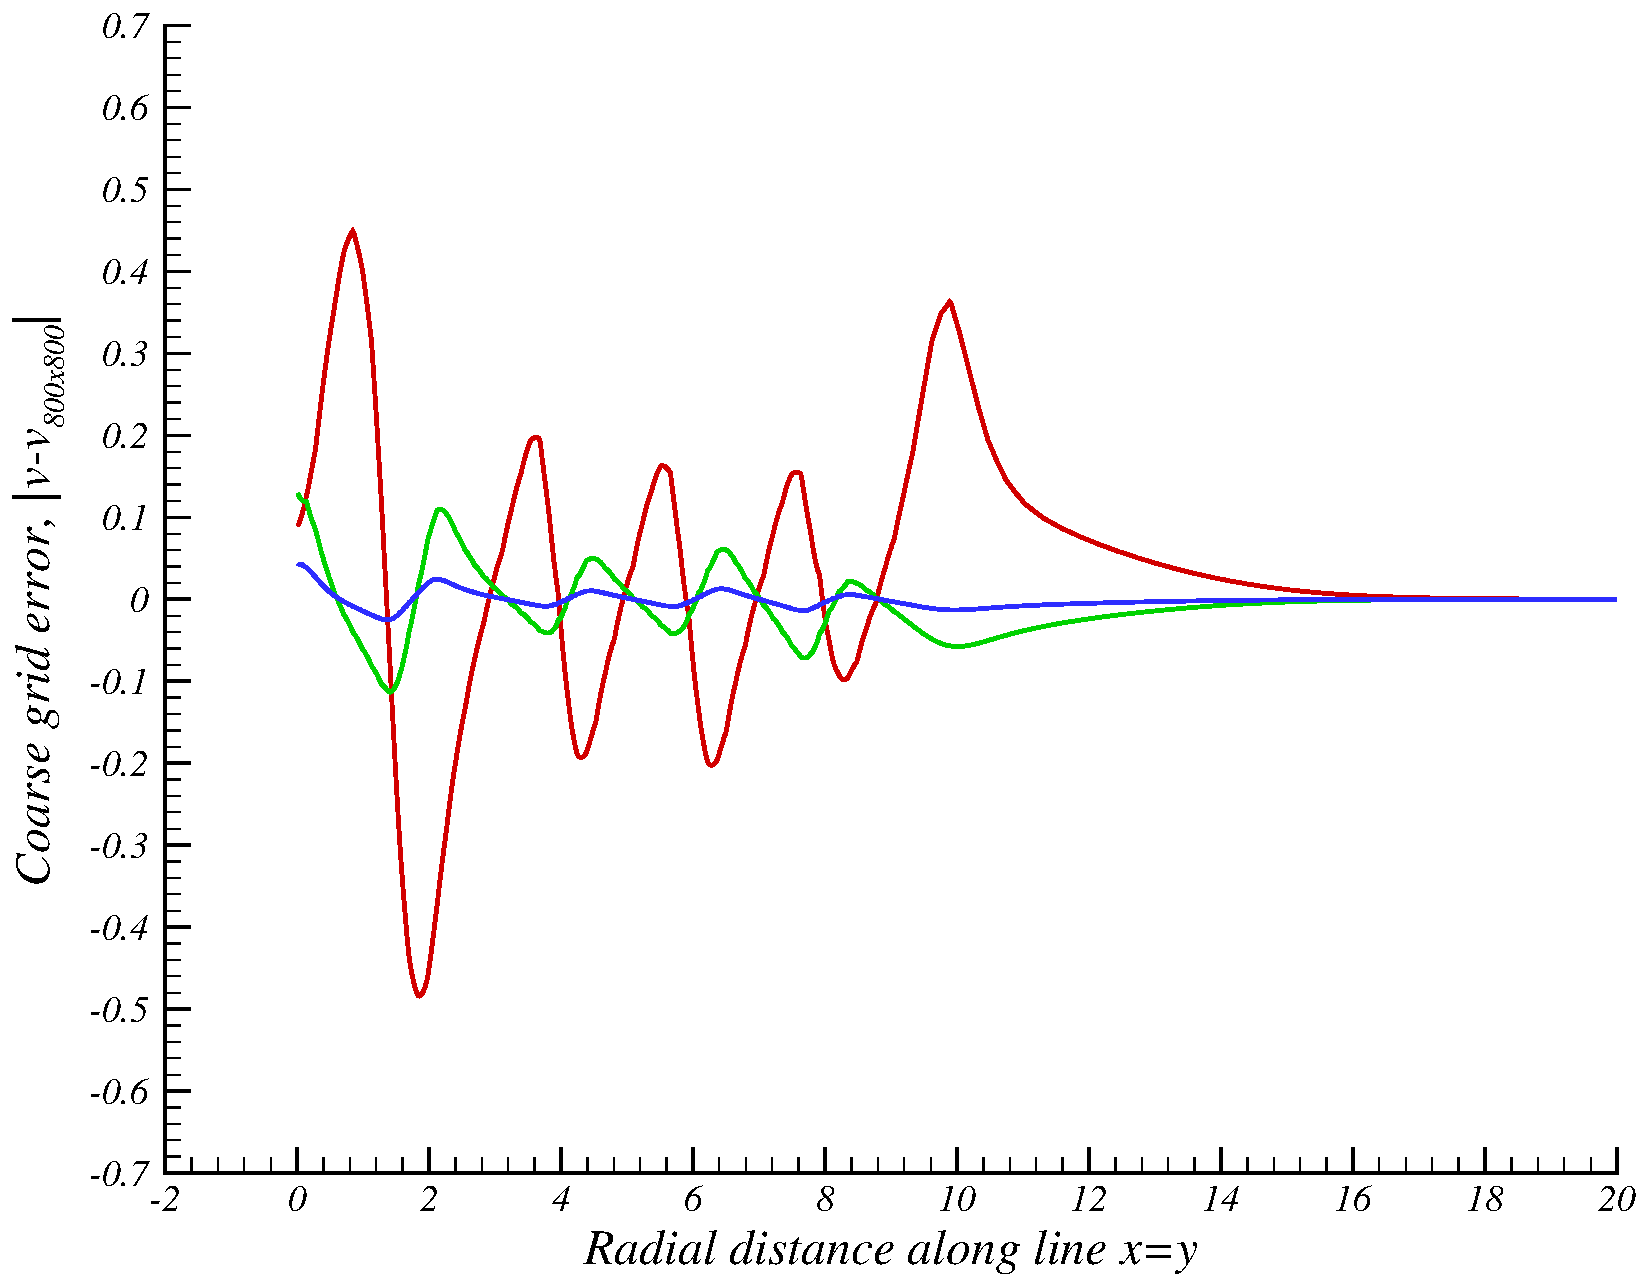
\includegraphics[height=.25\textheight]{figures/bio_concentric_rings/err_v_00016}}
    \subfigure[t=22.5]{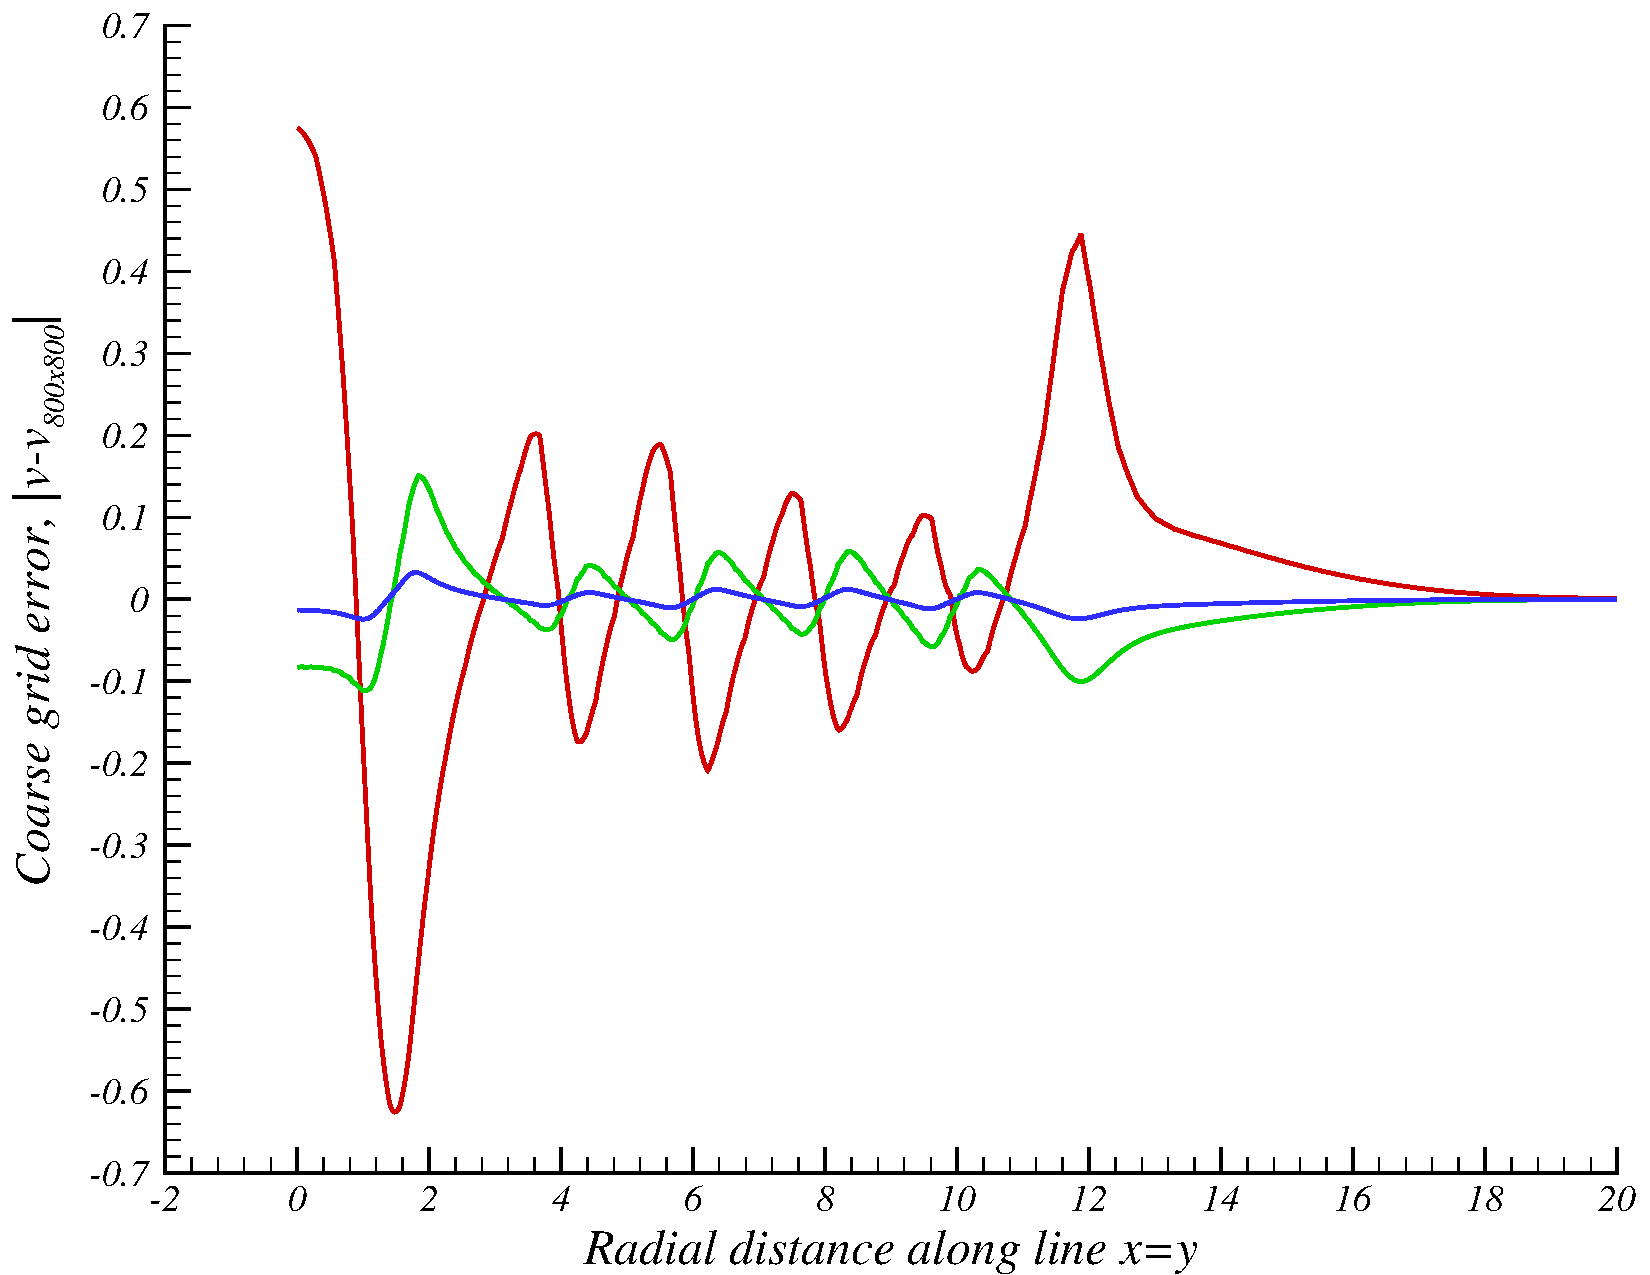
\includegraphics[height=.25\textheight]{figures/bio_concentric_rings/err_v_00018}} \\
    \subfigure[t=25.0]{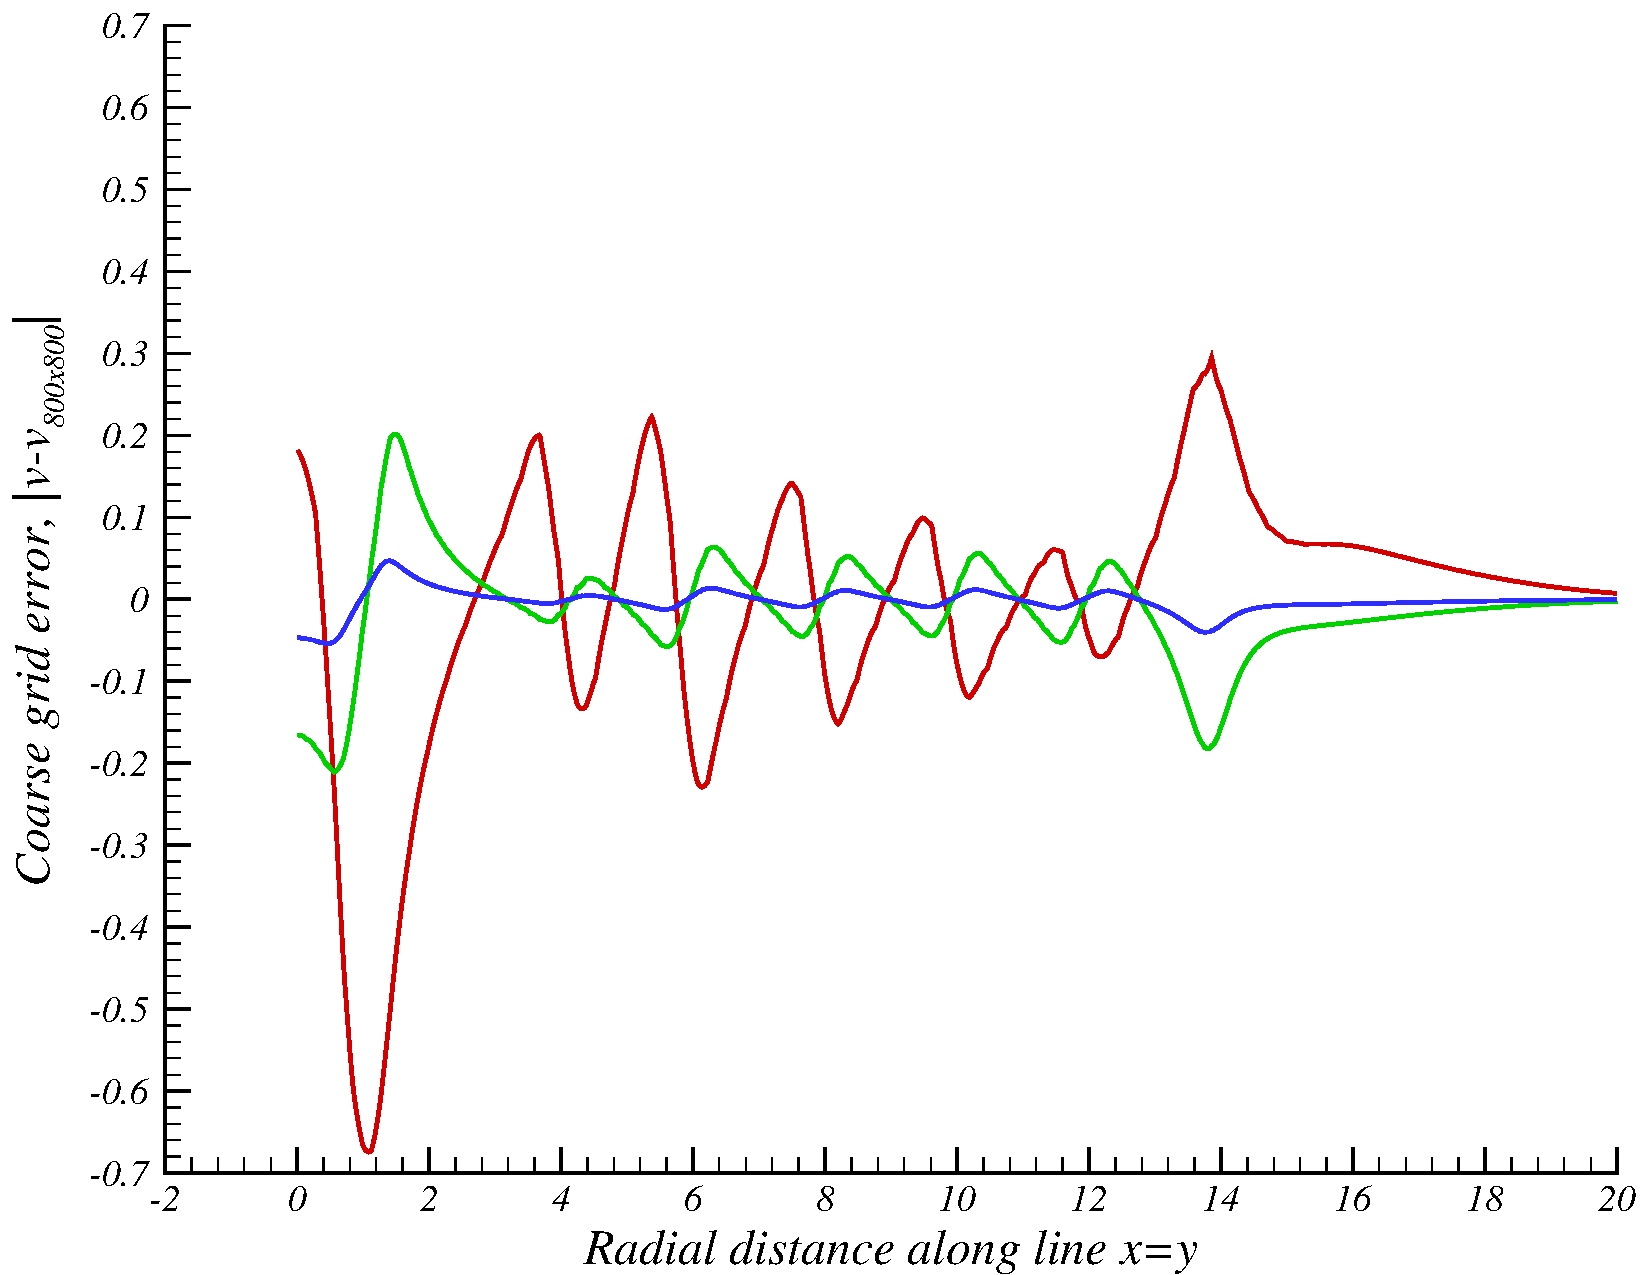
\includegraphics[height=.25\textheight]{figures/bio_concentric_rings/err_v_00020}}
    \subfigure[t=27.5]{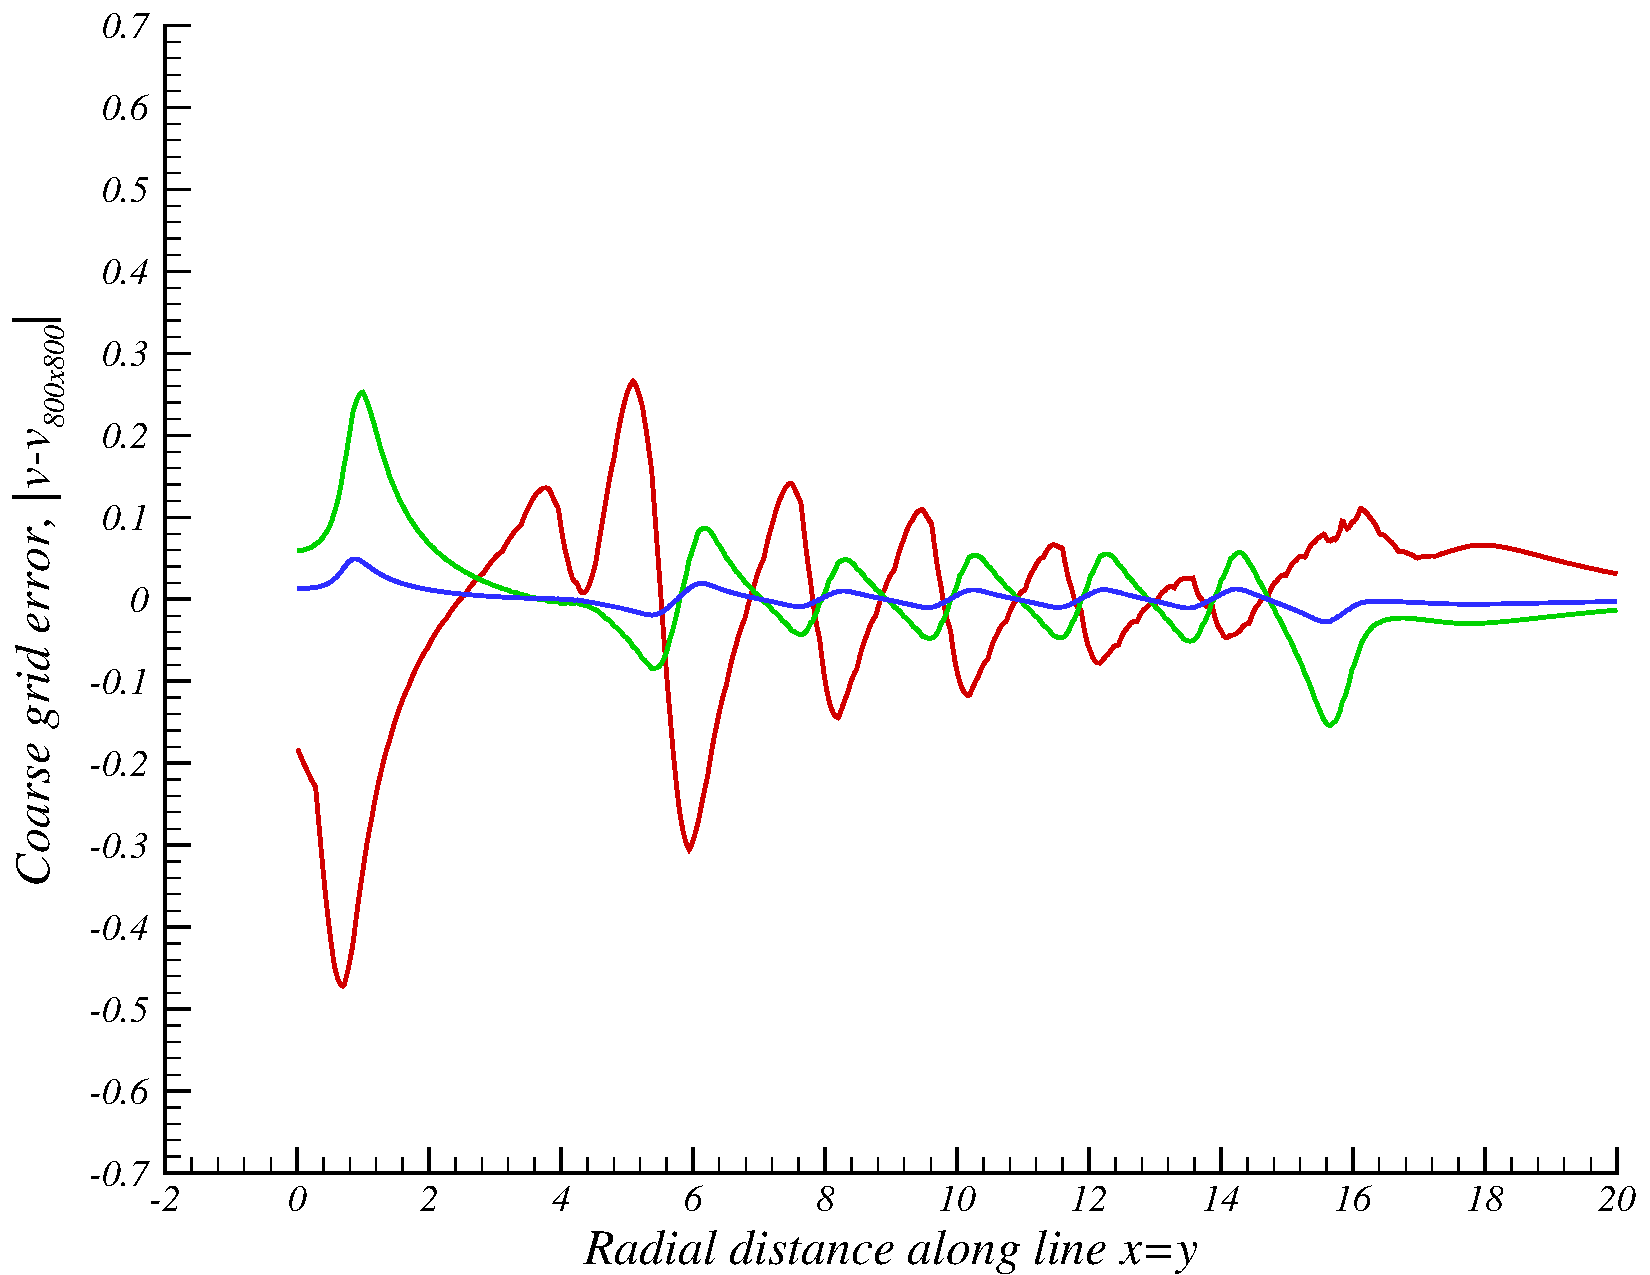
\includegraphics[height=.25\textheight]{figures/bio_concentric_rings/err_v_00022}}
    \caption{Continuous concentric advancing rings. Coarse grid chemoattractant concentration error history.\label{fig:bio_concentric_rings_chemoattractant_error}}
  \end{center}
\end{figure}

The figures reinforce the previous observation that the $100\times 100$ results are completely erroneous.  This is clear because the coarse grid error, $(u_{100\times 100} - u_{800\times 800})$ is of the same order of magnitude as the solution value itself, i.e. the coarse grid solution is not accurate to any significant digits.

The error for the $200\times 200$ and $400\times 400$ meshes is markedly decreased.  Inspection of Figures~\ref{fig:bio_concentric_rings_bacteria_error} and~\ref{fig:bio_concentric_rings_chemoattractant_error} shows that the error for these two solutions follows the same trend.  This is consistent with the previous observation that the solution is approaching mesh convergence for these resolutions. 

\subsubsection{Adaptive Mesh Refinement}
It is clear from Figures~\ref{fig:bio_concentric_rings_bacteria_error}--\ref{fig:bio_concentric_rings_chemoattractant_error} that the domain is largely quiescent for $t<15$.  For these early times the uniform Cartesian meshes considered previously are clearly ``wasteful'' since the fine mesh is only needed in the central, active subregion.  To assess the viability of adaptive mesh refinement for this application the simulation was repeated with AMR beginning from a background $25\times 25$ mesh.  The maximum refinement level is restricted to four, which would correspond to a uniform $400 \times 400$ mesh.  The adapted mesh is shown at two distinct times in Figure~\ref{fig:bio_concentric_rings_amr}.
\begin{figure}
  \begin{center}
    \subfigure{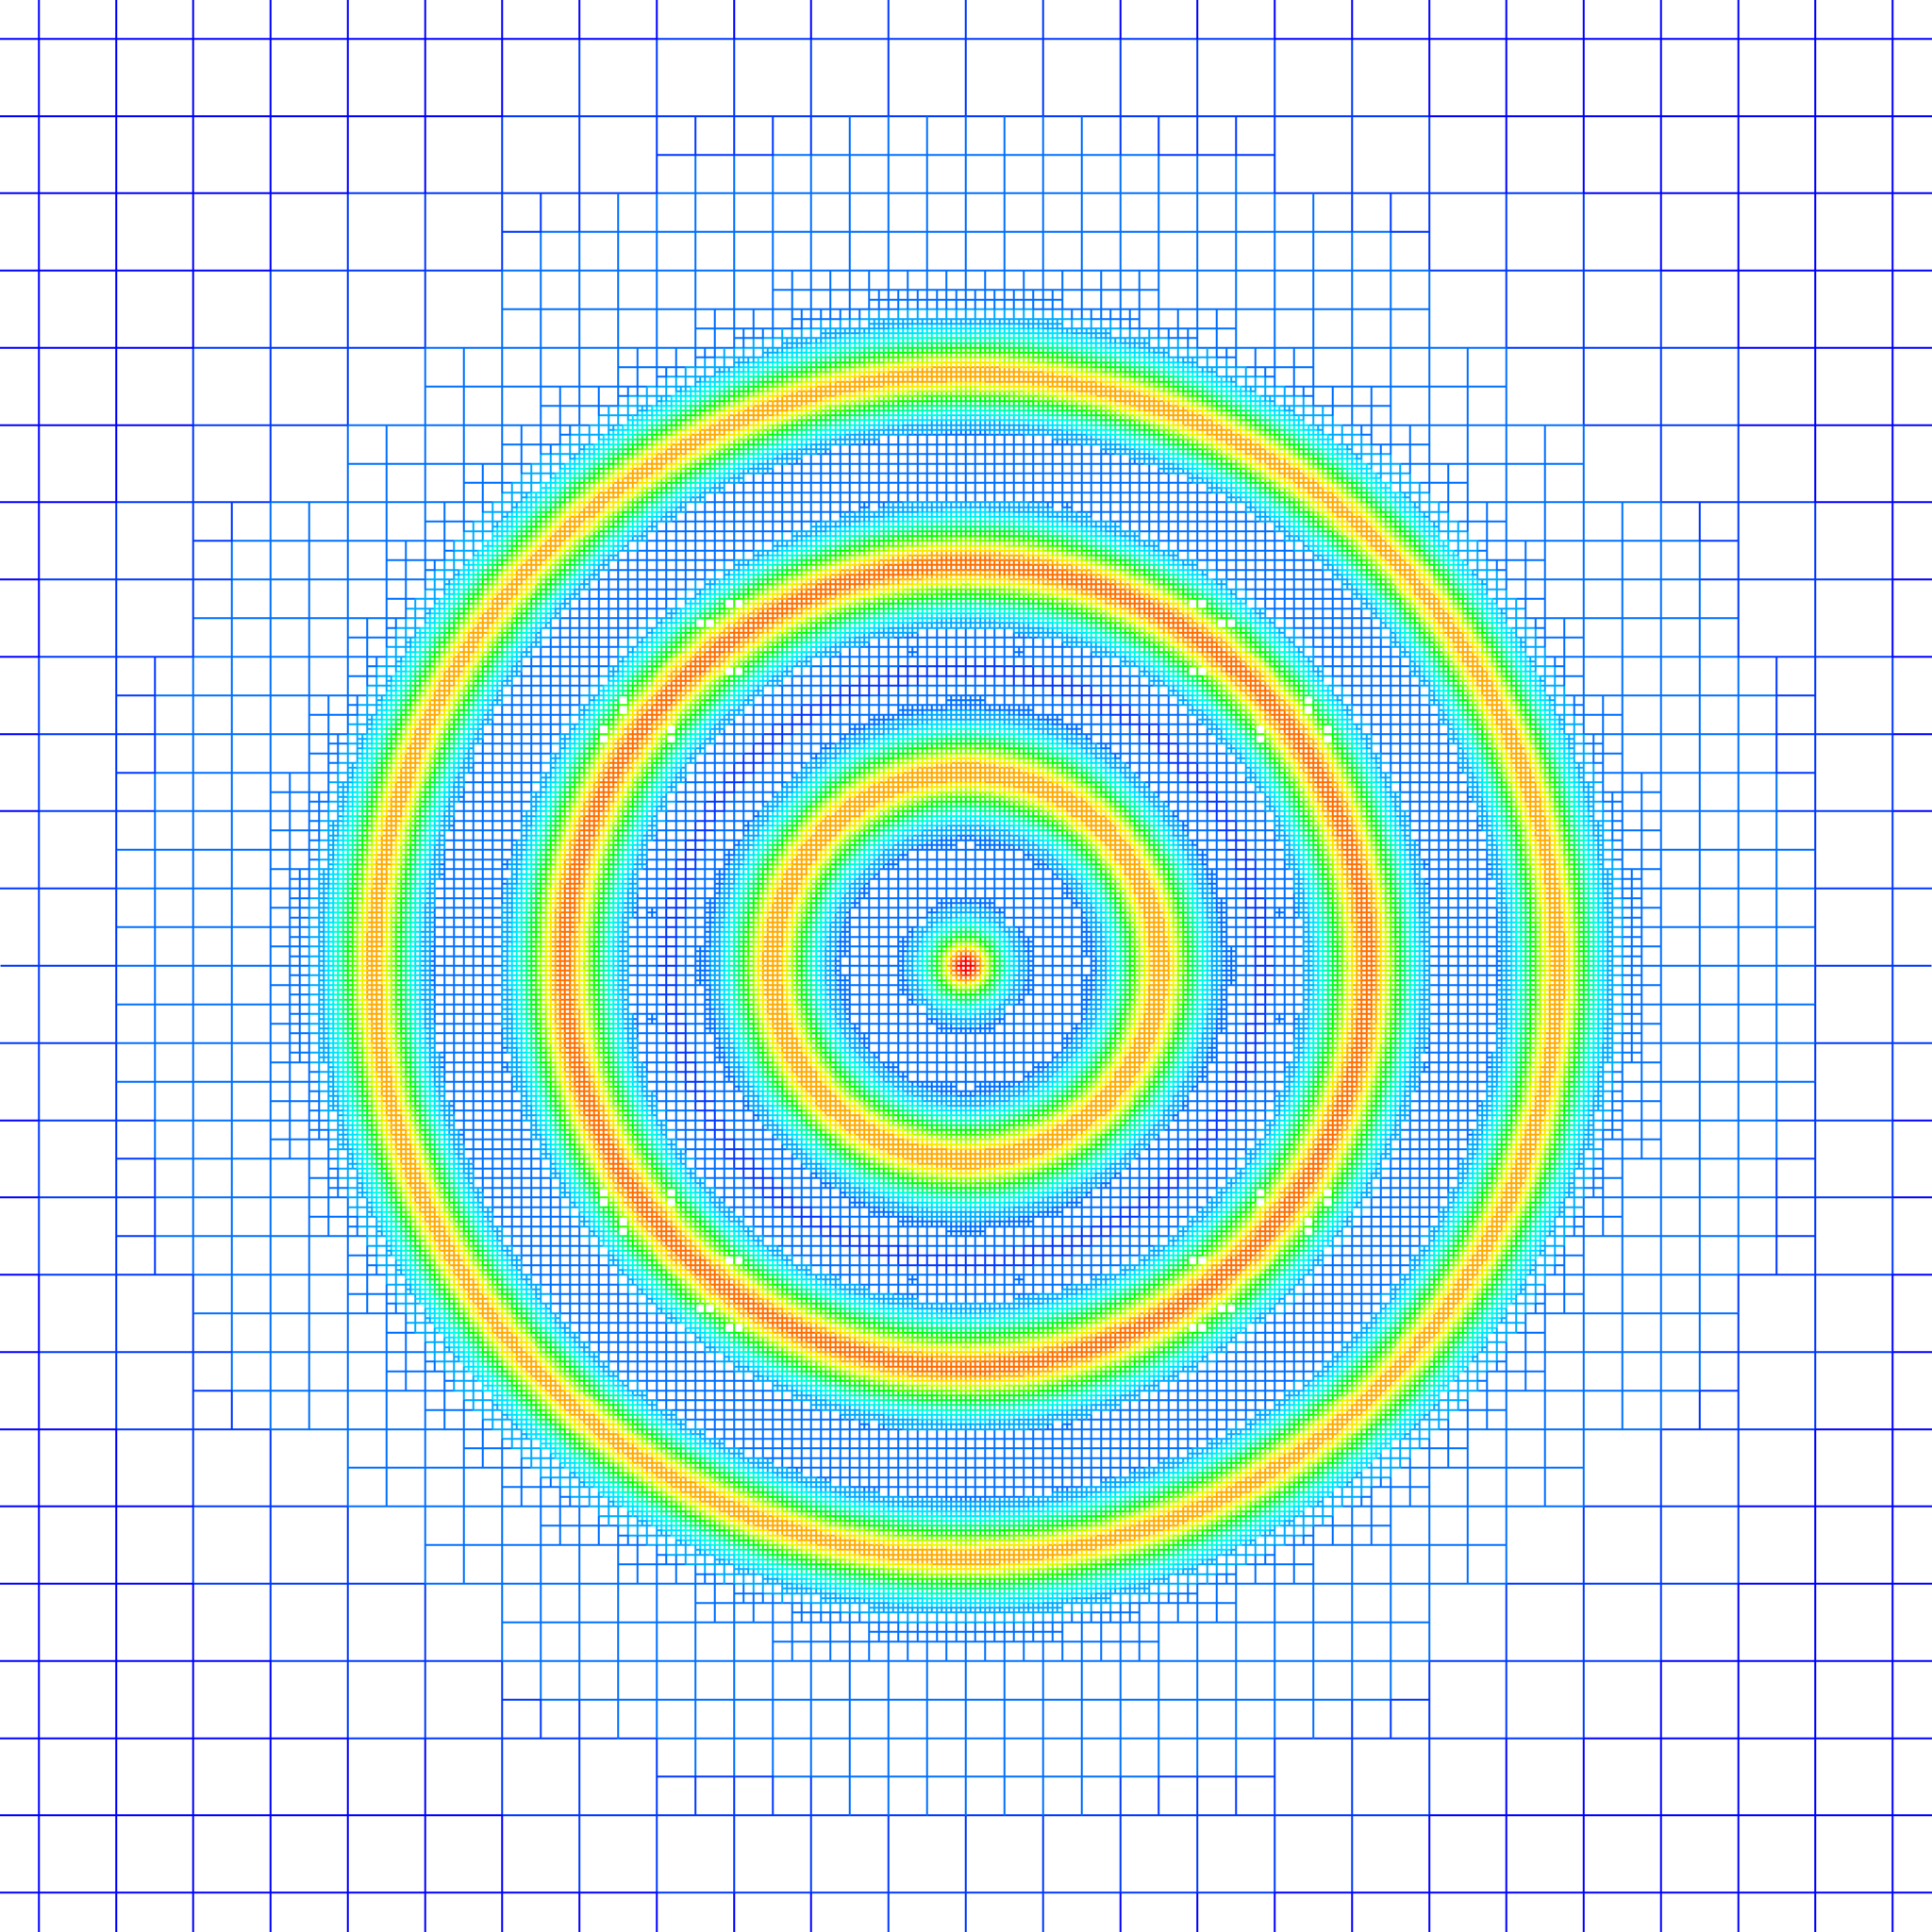
\includegraphics[height=.42\textheight]{figures/bio_concentric_rings/amr1}} \\
    \subfigure{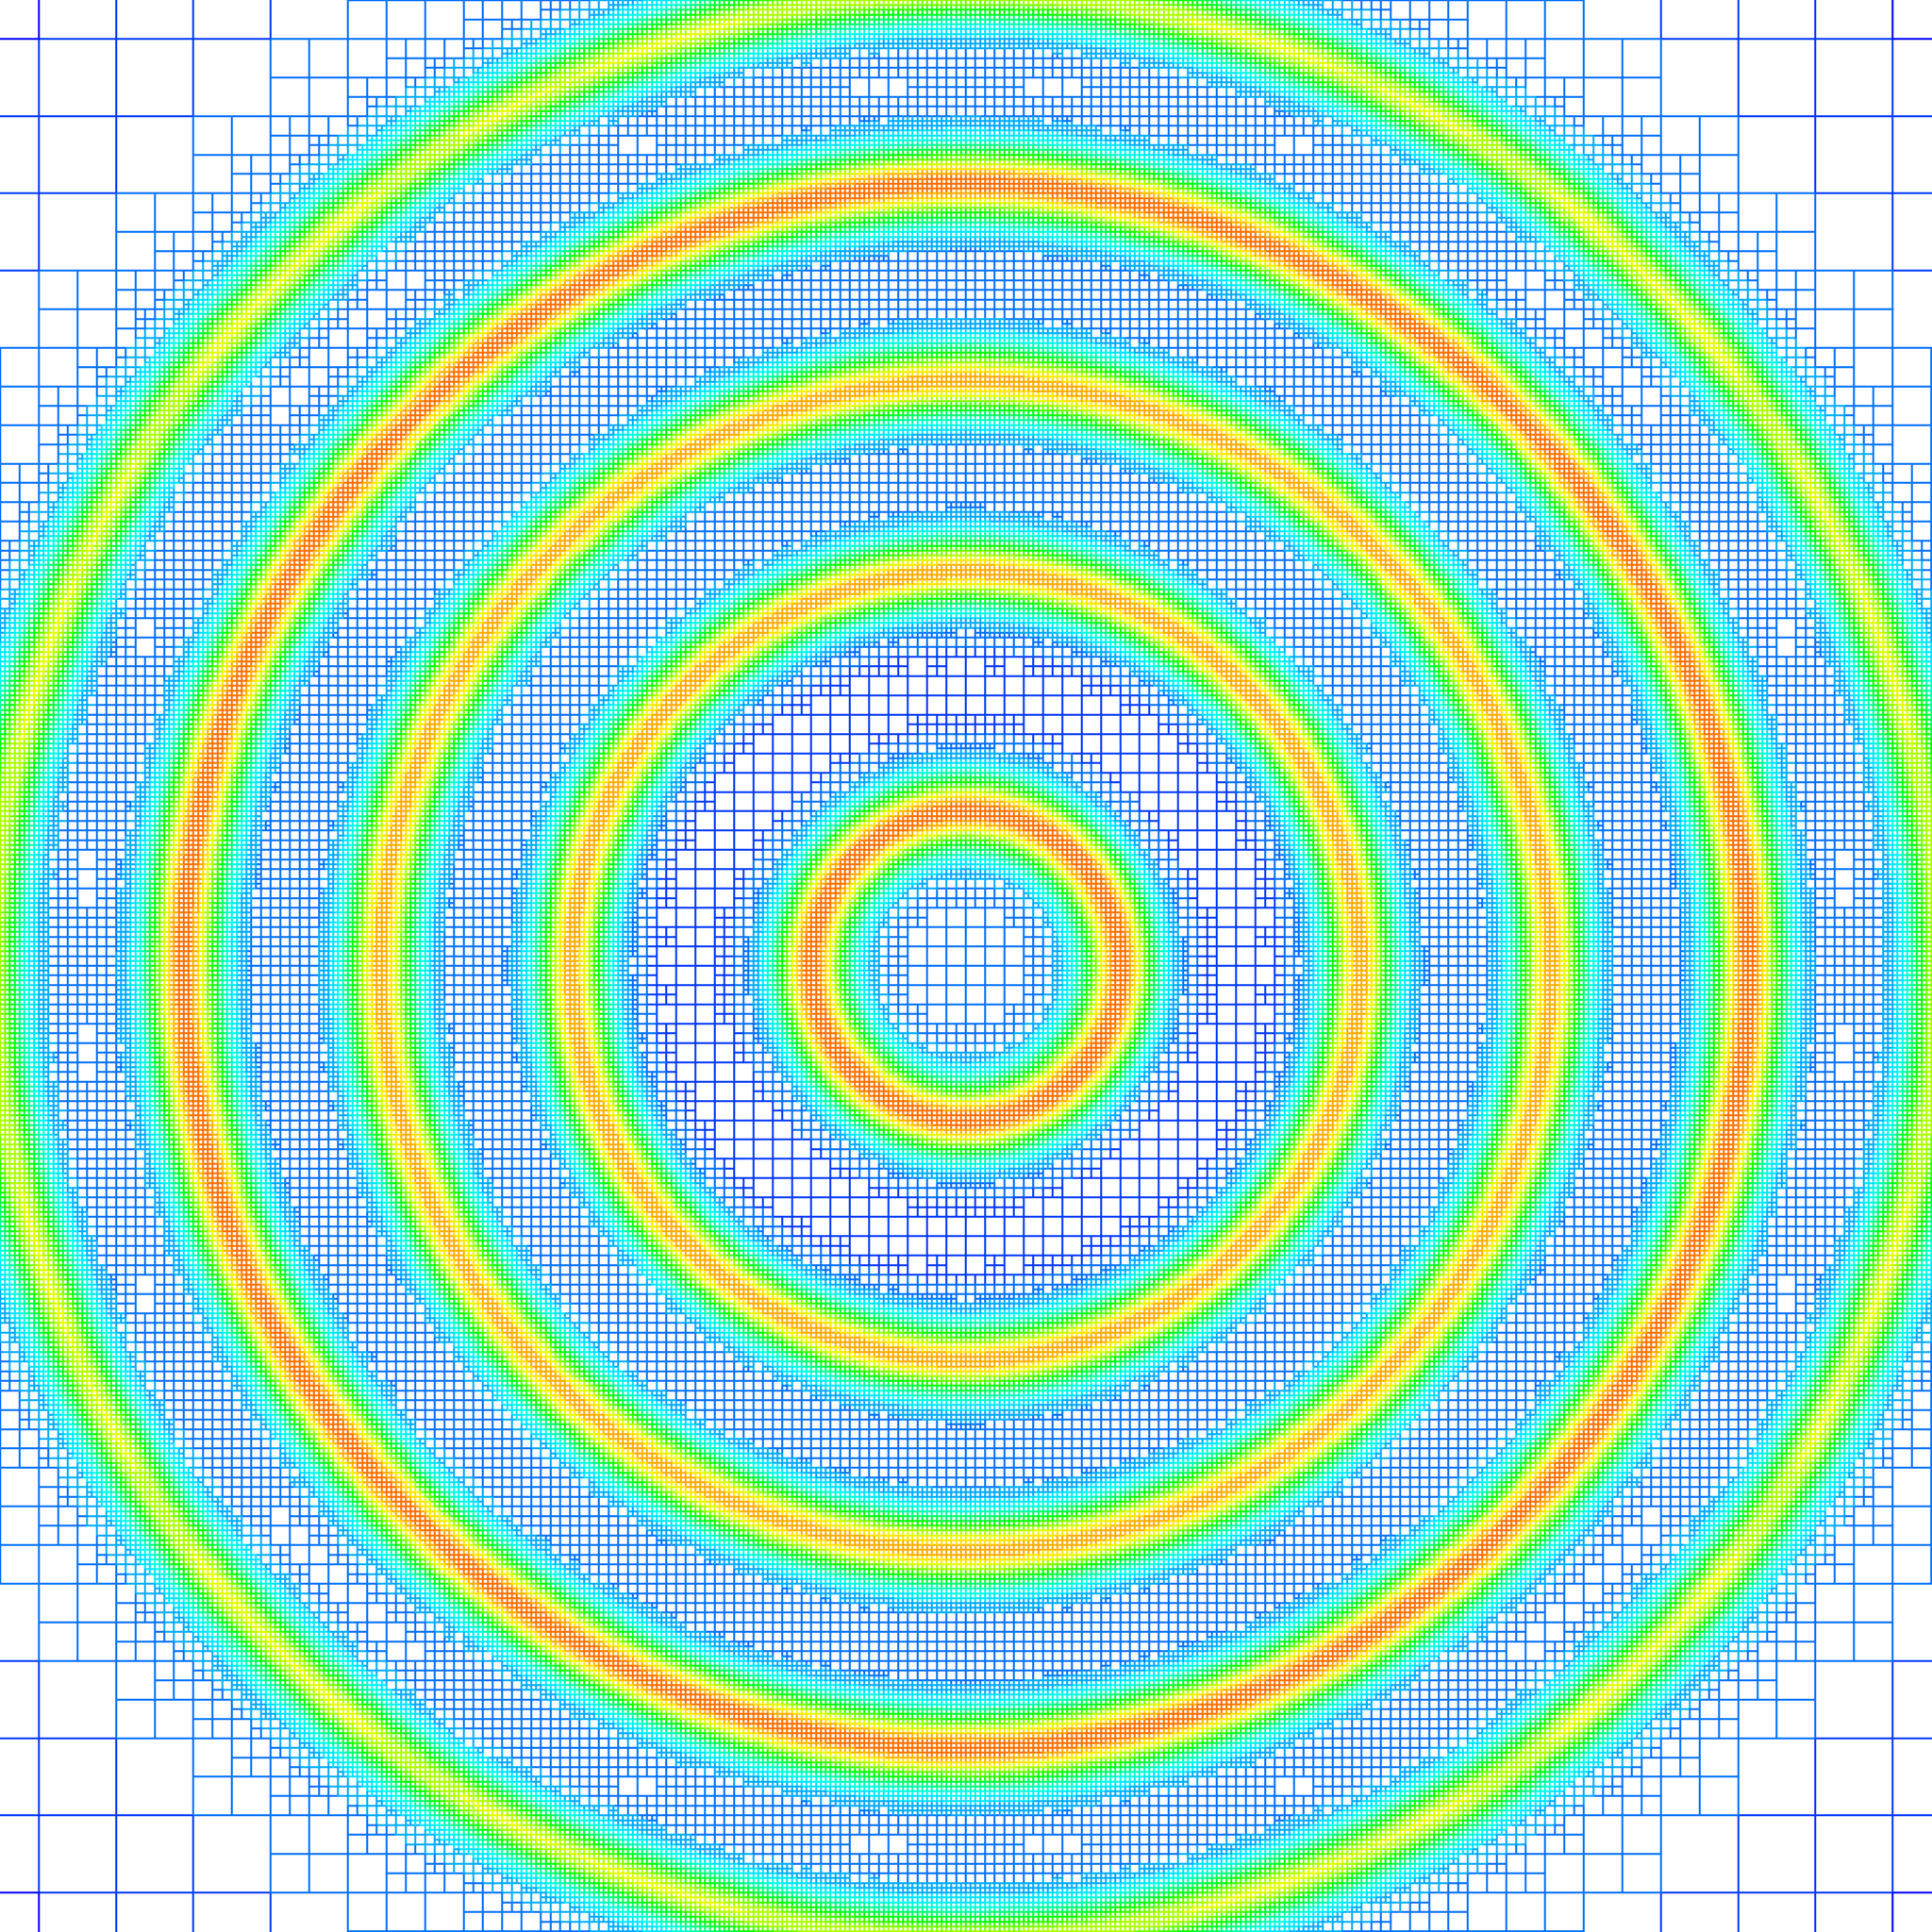
\includegraphics[height=.42\textheight]{figures/bio_concentric_rings/amr2}}
    \caption[Continuous concentric advancing rings.  Locally refined mesh for two instances in time.]{Continuous concentric advancing rings.  Locally refined mesh for two instances in time.  The mesh in the $[-10,10]^2$ region of interest is colored by bacteria concentration.\label{fig:bio_concentric_rings_amr}}
  \end{center}
\end{figure}
The gradient indicator does an excellent job tracking the high curvature regions of the rings.

The number of degrees of freedom as a function of time step is shown in Figure~\ref{fig:bio_concentric_rings_amr_dofs}.
\begin{figure}
  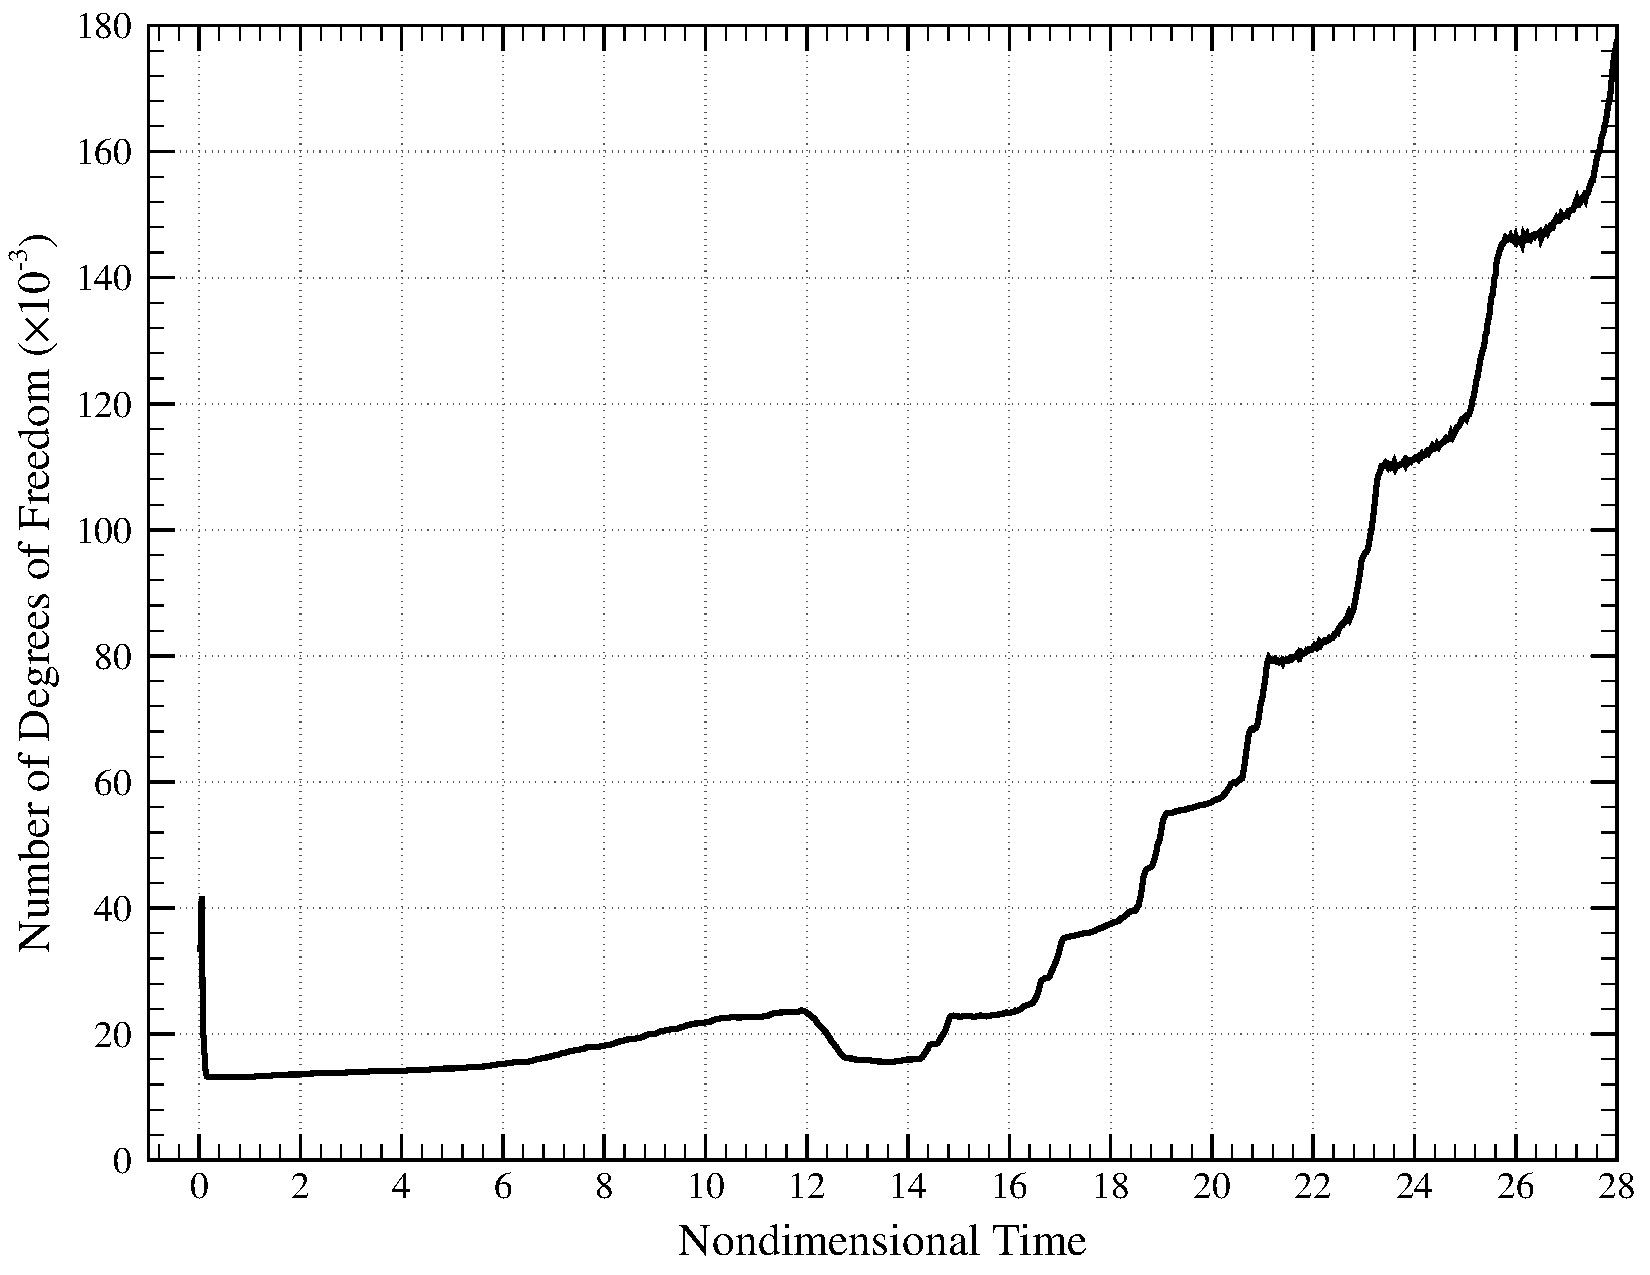
\includegraphics[width=\textwidth]{figures/bio_concentric_rings/dofs}
  \caption{Continuous concentric advancing rings. Number of degrees of freedom as a function of time for the adaptive simulation.\label{fig:bio_concentric_rings_amr_dofs}}
\end{figure}
Recall that by limiting the element refinement to four levels a fine-grid spacing consistent with a $400 \times 400$ uniform Cartesian mesh results.  Such a uniform mesh would result in a total of 482,403 degrees of freedom for the entire duration of the simulation.  The tremendous savings afforded by the adaptive approach are clear from the figure.  The largest problem size in the case of the adaptive mesh is more than a factor of two smaller than the equivalent uniform mesh.  Further, for much of the simulated time the number of degrees of freedom is less than 40,000 -- a factor of \emph{ten} fewer degrees of freedom than in the uniform mesh case.


%\subsubsection{Observations}

%%%%%%%%%%%%%%%%%%%%%%%%%%%%%%%%%%%%%%%%%%%%%%%%%%%%%%%%%%%%%%%%%%%%%%%%%%%%%%%
%\clearpage
\subsection{Radial Spots Behind an Advancing Swarm Ring\label{sect:radial_spots}}

\subsubsection{Domain Specification and Initial Conditions}
The initial conditions for this problem physically correspond to an initial inoculum of bacteria located at the center of a square domain which is defined as $\Omega=[-15,15]^2$.  As in the previous case, the domain is initially devoid of chemoattractant and has a uniform food source distribution. Also, symmetry is again assumed so that only a quarter-domain is simulated.

The initial nondimensional bacteria concentration for this case is $u_0=1$.  As discussed in Section~\ref{sec:concentric_rings}, it is again important that $u_0$ be specified in such a way that it can be implemented consistently across a range of mesh resolutions and element types. For this problem the same sequence of uniformly refined meshes with both bilinear and biquadratic elements to test mesh convergence.  The coarsest mesh contains $100\times100$ elements, yielding a coarse mesh spacing of $h_c=0.15$. For this family of meshes the initial conditions are taken as a tensor product of the following one-dimensional distributions:
\begin{alignat}{2}
  u_0 & = 1                 & \qquad & x \le h_c     \label{eq:u0_1_radial_spots} \\
      & = 2 - \frac{x}{h_c} & \qquad & h_c < x < 2hc \label{eq:u0_2_radial_spots} \\
      & =0                  & \qquad & x \ge 2hc     \label{eq:u0_3_radial_spots} \\
      &                     &        & \nonumber \\  
  v_0 & =0                  &        &               \label{eq:v0_radial_spots}   \\
      &                     &        & \nonumber \\  
  w_0 & =\frac{8}{10}       &        &               \label{eq:w0_radial_spots}   
\end{alignat}
%% In particular, the linear decay of initial bacteria concentration specified by Equation~\eqref{eq:u0_2_radial_spots} is chosen because it can be represented exactly with the bilinear and biquadratic elements for the full range of mesh resolutions used in this study.
%% \begin{figure}[hbtp]
%%   \begin{center}
%%     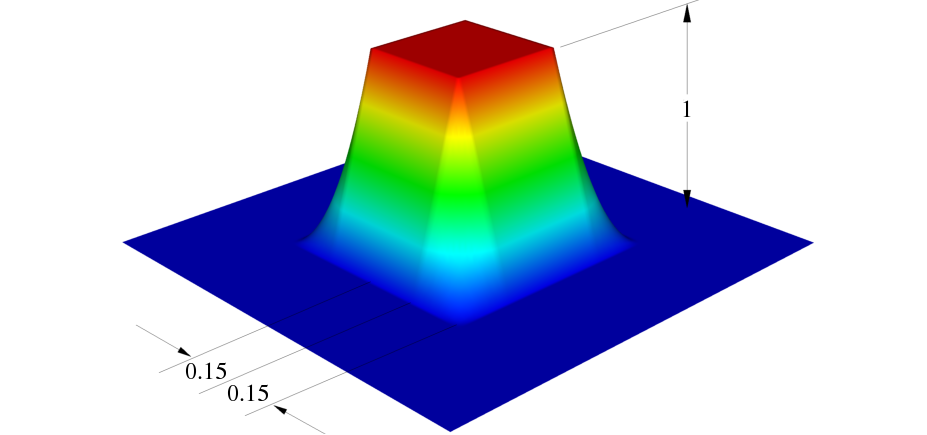
\includegraphics[width=\textwidth]{figures/bio_radial_spots/u0_schematic}
%%     \caption{Initial bacteria concentration for the swarm ring problem\label{fig:u0_radial_spots}}
%%   \end{center}
%% \end{figure}
%% Also, by fixing the slope of the decay for all mesh resolutions initial transients caused by inconsistent initial conditions are avoided.  The resulting two-dimensional initial bacteria concentration is shown in Figure~\ref{fig:u0_radial_spots}.

\subsubsection{System Parameters}
% Parameter values - biological problem no. 2:  swarm ring
\begin{table}[hbtp]
  \begin{center}
    \caption[Nondimensional parameter values for radial spots deposited behind an advancing swarm ring]{Nondimensional parameter values for radial spots deposited behind an advancing swarm ring (from Woodward et~al.~\cite{spatio_temporal_patterns})}
    \label{table:radial_spots_parameters}
    \vspace{1em}
    \begin{tabular}{cccccccc} \hline \hline
      $\bv{d_u}$ & $\bv{d_w}$ & $\bv{\alpha}$ & $\bv{\beta}$ & $\bv{\delta}$ & $\bv{\rho}$ & $\bv{\mu}$ & $\bv{\kappa}$ \\
      \unitfrac{1}{4}       & 1          & 30            & 10           & \unitfrac{7}{2}           & 1           & 50         & 0             \\ \hline
    \end{tabular}
  \end{center}
\end{table}
The relevant parameters for this case were taken from Woodward et~al.~\cite{spatio_temporal_patterns} and are listed in Table~\ref{table:radial_spots_parameters}. The value $\alpha=30$, which weights the chemotaxis term, is large enough for the system to exhibit appreciable chemotaxis-induced bacteria transport.  Specifically for this choice of parameters, equations~\eqref{eq:pde_bio_u}--\eqref{eq:pde_bio_w} become
% Bacterial chemotaxis: swarm ring problem, 1st simplification
\begin{align}
  \label{eq:pde_bio_u_radial_spots_1}
  \frac{\partial u}{\partial t} & = \frac{1}{4} \Delta u - 30 \; \grad{}\cdot \left[ \frac{u}{(1+ v)^2} \grad{v} \right]
                                    + \frac{7 \; u}{2} \left( \frac{w^2}{1 + w^2} - u \right) \\
  \label{eq:pde_bio_v_radial_spots_1}
  \frac{\partial v}{\partial t} & = \;\;\Delta v + \frac{10 \; w u^2}{50 + u^2} - uv \\
  \label{eq:pde_bio_w_radial_spots_1}
  \frac{\partial w}{\partial t} & = \;\;\Delta w 
\end{align}
In particular, the parameter $\kappa=0$ again decouples the stimulant concentration ($w$) from the bacterial ($u$) and chemoattractant ($v$) concentrations. %The physical interpretation of this scenario is that the stimulant supply is essentially unlimited, and its distribution is influenced only though diffusion.  Particularly, the bacteria cannot deplete the stimulant source, no matter how densely populated a region may be.  Additionally, since the stimulant is uniformly distributed initially, even diffusion will be absent for this particular case.  In this scenario the stimulant distribution is completely defined its initial value, and
The governing equations reduce to
% Bacterial chemotaxis: swarm ring problem, 2nd simplification
\begin{align}
  \label{eq:pde_bio_w_radial_spots_2}
  w &= \frac{8}{10} \\
  \label{eq:pde_bio_u_radial_spots_2}
  \frac{\partial u}{\partial t} & = \frac{1}{4} \Delta u - 30 \; \grad{}\cdot \left[ \frac{u}{(1+ v)^2} \grad{v} \right]
                                    + u \left( \frac{56}{41} - u \right) \\
  \label{eq:pde_bio_v_radial_spots_2}
  \frac{\partial v}{\partial t} & = \;\;\Delta v + \frac{8 \; u^2}{50 + u^2} - uv
\end{align}
As mentioned previously, the decoupling of the governing equations when $\kappa=0$ could be exploited numerically to reduce storage requirements.

\subsubsection{Mesh and Time Convergence Studies}
This section presents the results of mesh and time convergence studies.  The goal of these studies was (i) to produce high-accuracy reference solutions and (ii) to determine the time accuracy required for the system.  These solutions will be used for comparison to validate the adaptive algorithm.  Additional simulations varied the approximation and quadrature orders to verify the accuracy of the scheme.

\paragraph{Mesh Convergence:} Simulations were performed on a sequence of uniformly refined meshes to ensure mesh convergence of the solution.  Figure~\ref{fig:radial_spots_mesh_convergence} shows bacteria and chemoattractant contours for uniform meshes of $100\times 100$, $200\times 200$, and $400\times 400$ elements.  The negligible difference between the two finest meshes shows that mesh convergence is obtained and that a $200\times 200$ element mesh is adequate for this problem.
\begin{figure}[hbtp]
  \begin{center}
    \subfigure[Bacteria]{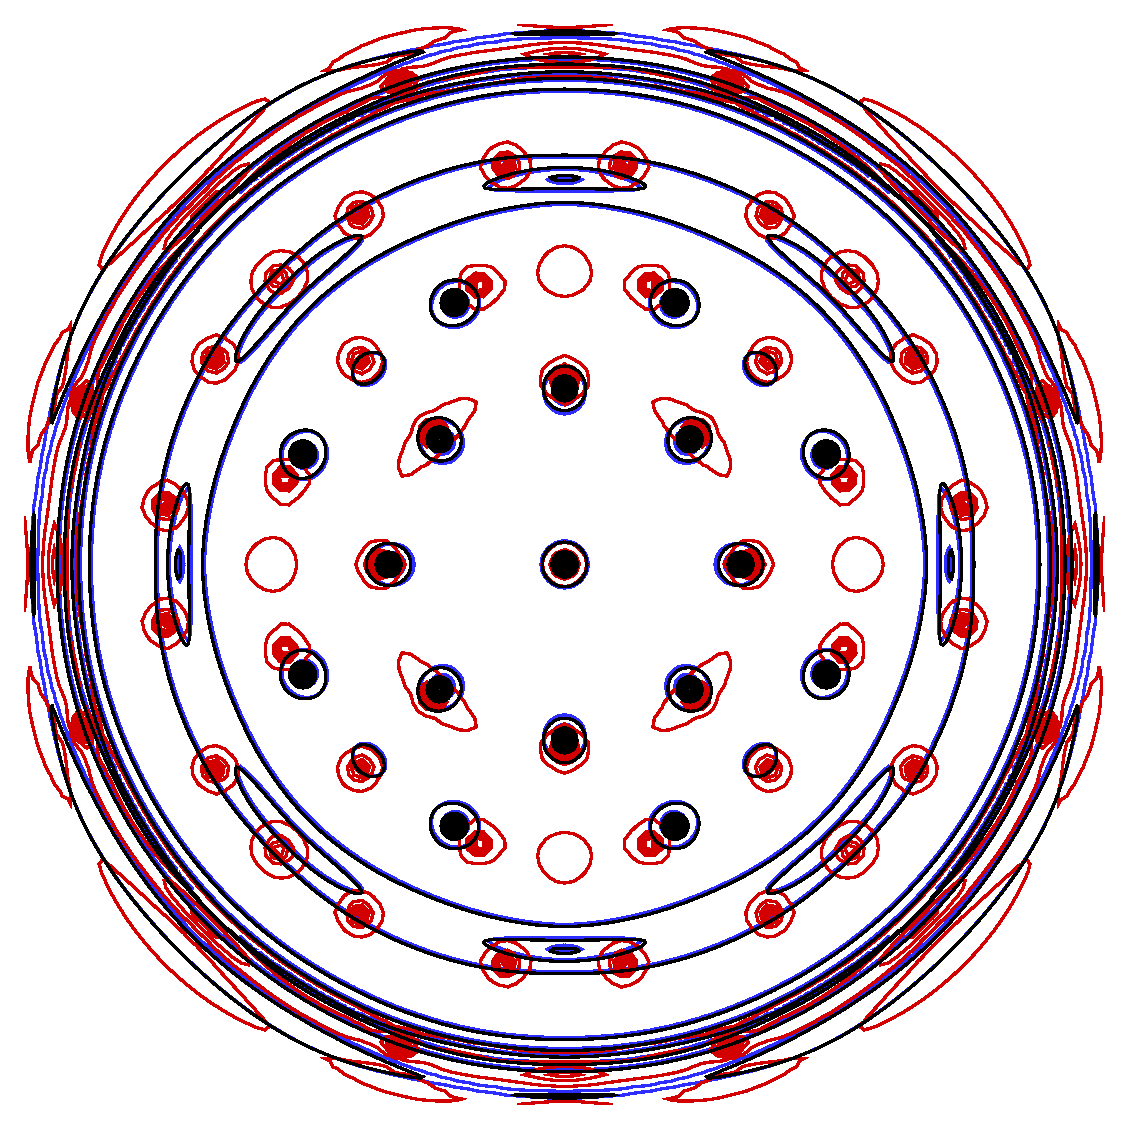
\includegraphics[width=.48\textwidth]{figures/bio_radial_spots/mesh_convergence/overlay_u}}
    \subfigure[Chemoattractant]{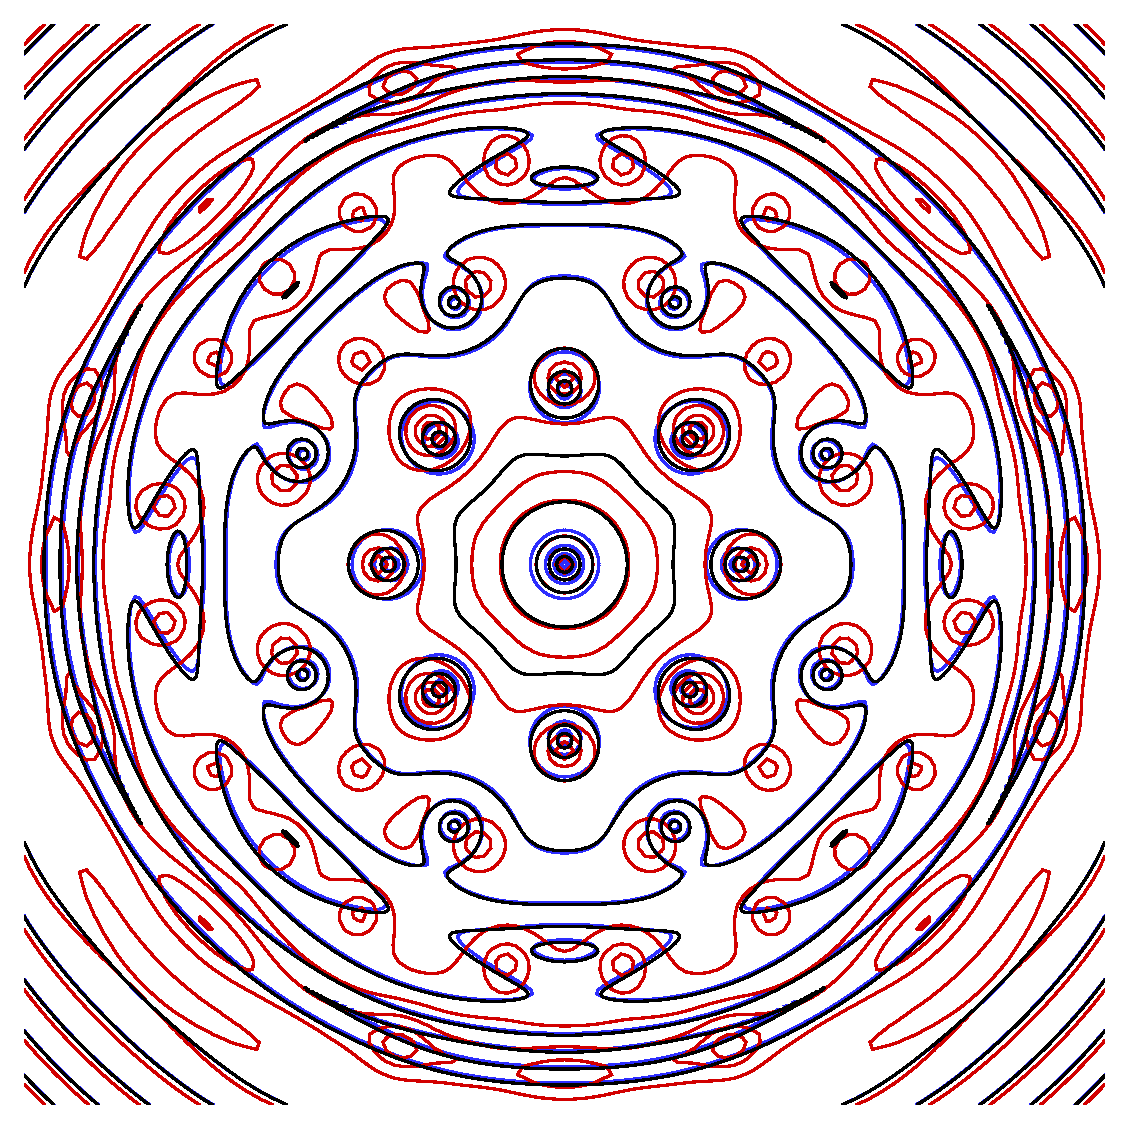
\includegraphics[width=.48\textwidth]{figures/bio_radial_spots/mesh_convergence/overlay_v}}
    \caption[Overlaid concentrations at $t=19$ on illustrating mesh convergence]{Overlaid concentrations at $t=19$ illustrating mesh convergence for \textcolor{red}{$100\times 100$}, \textcolor{blue}{$200\times 200$}, and $400\times 400$ uniform meshes.  The region of interest is a $[-10,10]^2$ subdomain.  Mesh convergence is obtained for the $200\times 200$ and finer meshes.\label{fig:radial_spots_mesh_convergence}}
  \end{center}
\end{figure}

\paragraph{Time Convergence:} Additional simulations were performed on a $200\times 200$ element mesh to investigate the time convergence of the solution. Figure~\ref{fig:radial_spots_time_convergence} shows bacteria and chemoattractant contours at a nondimensional time of $t=19$.  For these cases the time accuracy tolerance $\varepsilon_t$ (Equation~\eqref{eq:dt_comp}) was varied.  The figure shows that time convergence is obtained for values of $\varepsilon_t \le 1\times 10^{-2}$.

\begin{figure}[hbtp]
  \begin{center}
    \subfigure[Bacteria]{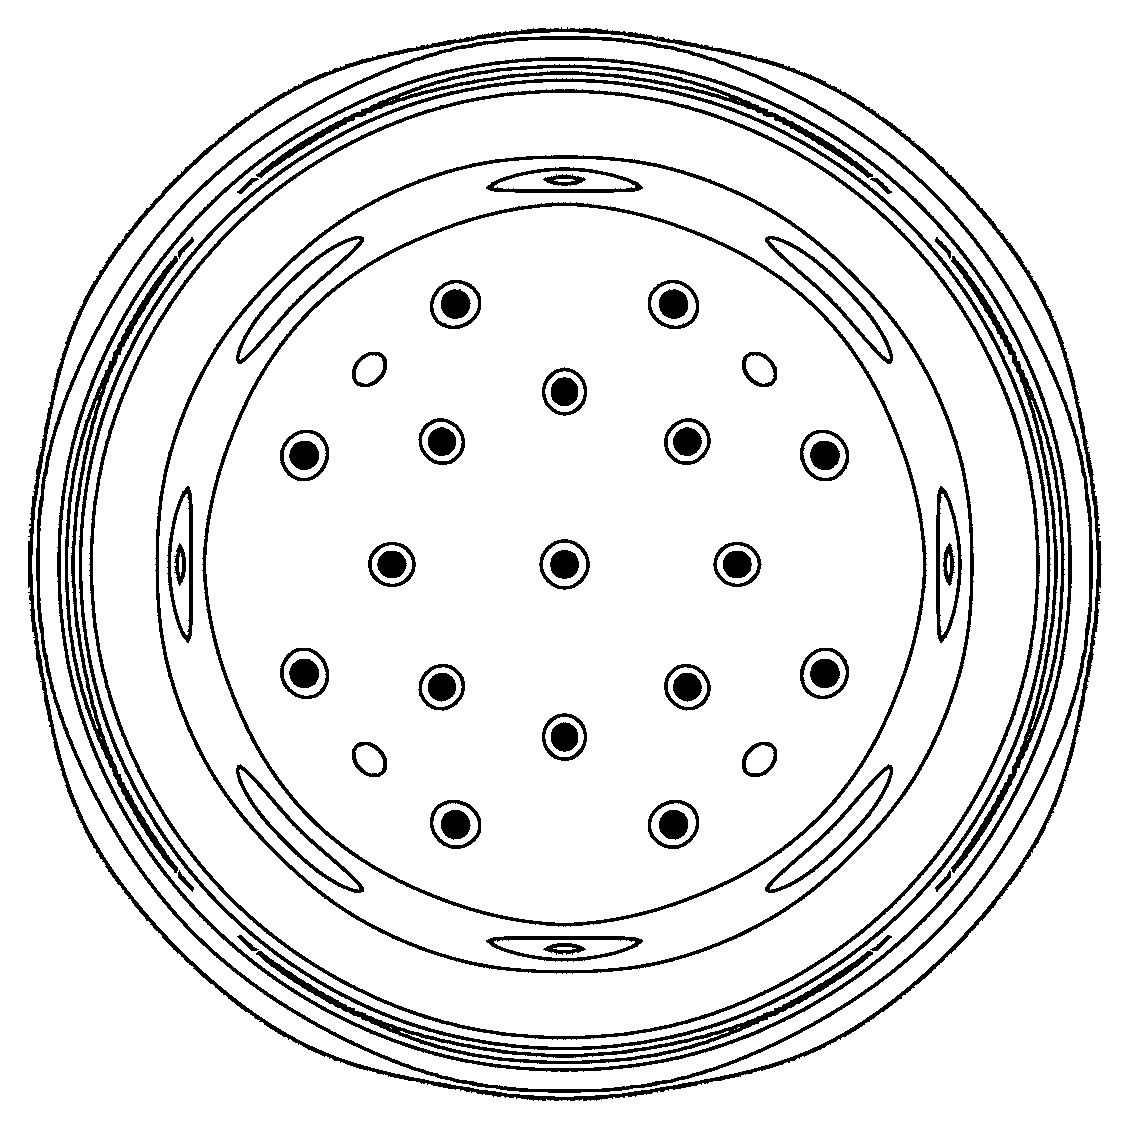
\includegraphics[width=.48\textwidth]{figures/bio_radial_spots/time_convergence/quad9_200x200/overlay_u}}
    \subfigure[Chemoattractant]{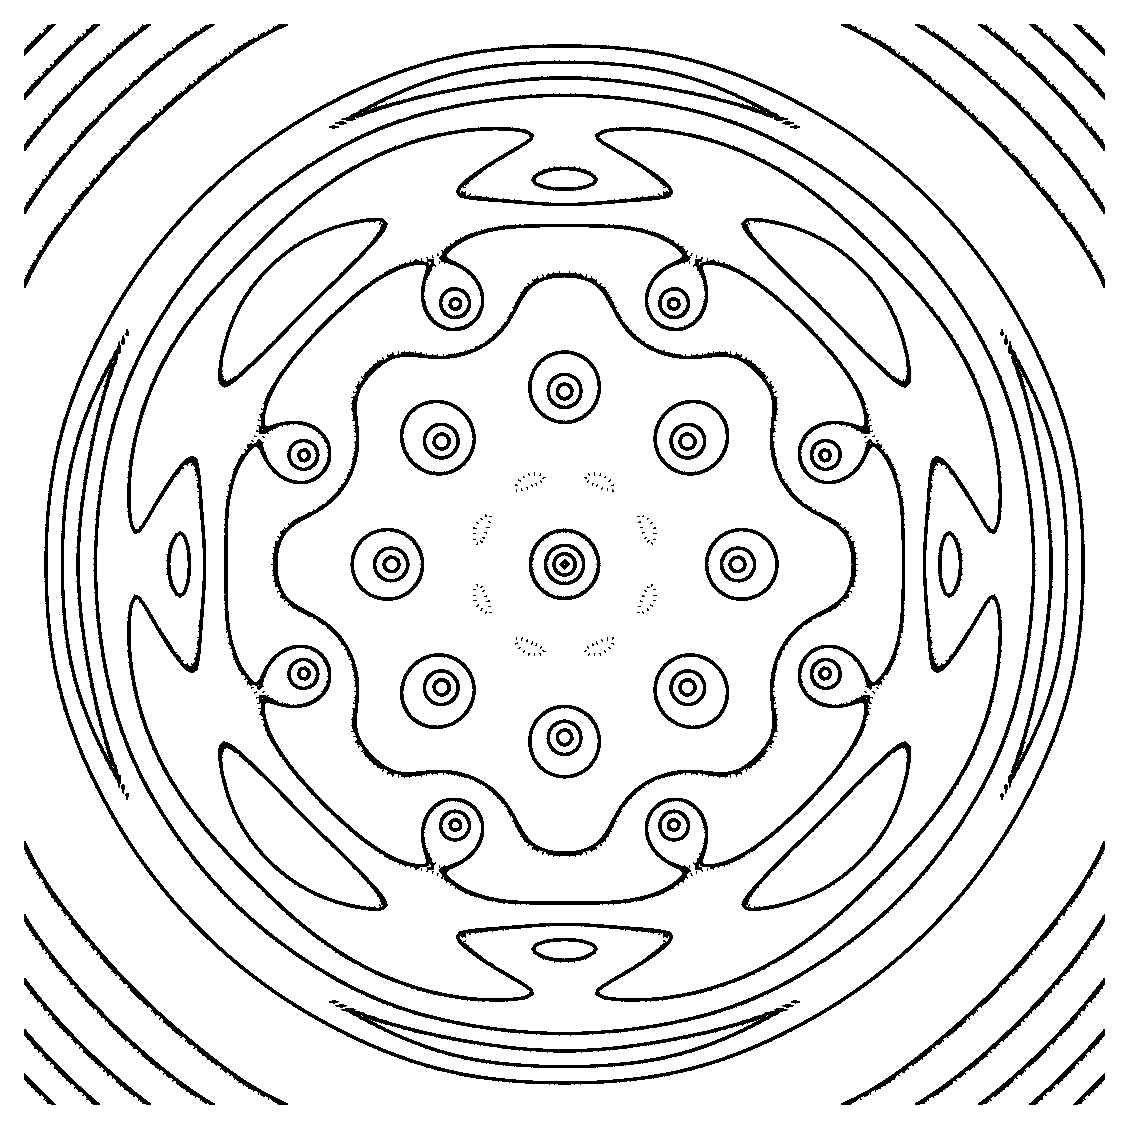
\includegraphics[width=.48\textwidth]{figures/bio_radial_spots/time_convergence/quad9_200x200/overlay_v}}
    \caption[Overlaid concentrations at $t=19$ on a $200\times 200$ uniform mesh illustrating time convergence]{Overlaid concentrations at $t=19$ on a $200\times 200$ uniform mesh illustrating time convergence for $\varepsilon_t=$\textcolor{black}{$2\times 10^{-2}$}, \textcolor{black}{$1\times 10^{-2}$}, \textcolor{black}{$5\times 10^{-3}$}, and $2.5\times 10^{-3}$.  The region of interest is a $[-10,10]^2$ subdomain.  Essentially all cases are time converged.\label{fig:radial_spots_time_convergence}}
  \end{center}
\end{figure}


\begin{figure}
  \begin{center}
    \subfigure[t=12.50]{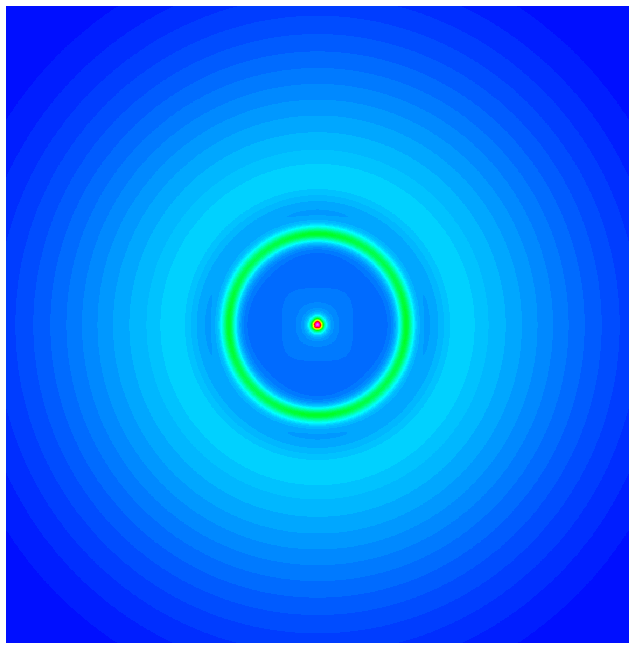
\includegraphics[height=.25\textheight]{figures/bio_radial_spots/u_00010}}
    \subfigure[t=13.75]{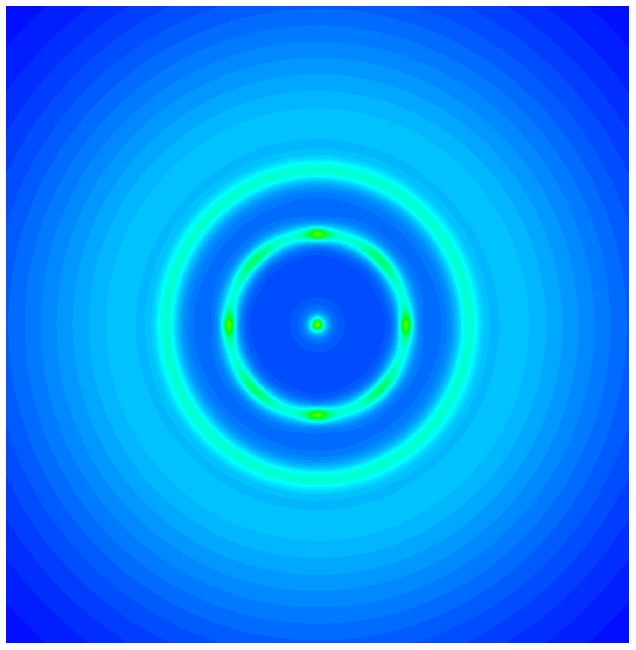
\includegraphics[height=.25\textheight]{figures/bio_radial_spots/u_00011}} \\
    \subfigure[t=15.00]{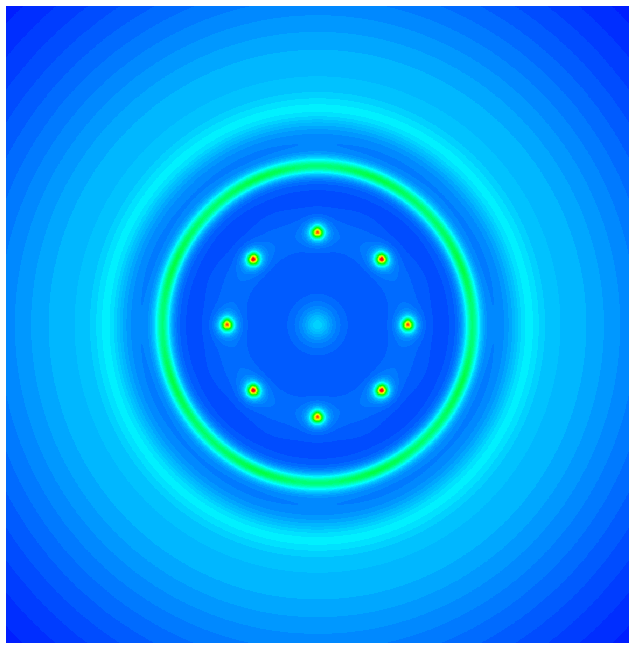
\includegraphics[height=.25\textheight]{figures/bio_radial_spots/u_00012}}
    \subfigure[t=16.25]{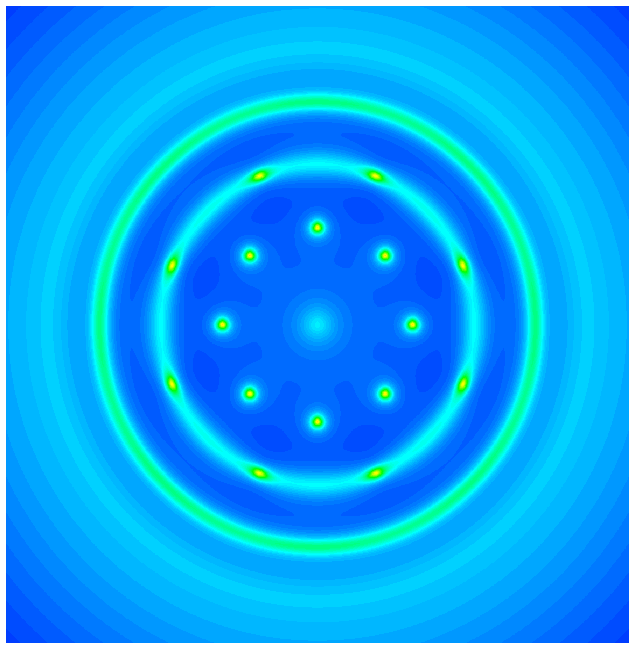
\includegraphics[height=.25\textheight]{figures/bio_radial_spots/u_00013}} \\
    \subfigure[t=17.50]{\includegraphics[height=.25\textheight]{figures/bio_radial_spots/u_00014}}
    \subfigure[t=18.75]{\includegraphics[height=.25\textheight]{figures/bio_radial_spots/u_00015}}
    \caption[Radial spots. Bacteria concentration history.]{Radial spots. Bacteria concentration history.  The region of interest is a $[-10,10]^2$ subdomain.\label{fig:bio_radial_spots_bacteria}}
  \end{center}
\end{figure}

\begin{figure}
  \begin{center}
    \subfigure[t=12.50]{\includegraphics[height=.25\textheight]{figures/bio_radial_spots/v_00010}}
    \subfigure[t=13.75]{\includegraphics[height=.25\textheight]{figures/bio_radial_spots/v_00011}} \\
    \subfigure[t=15.00]{\includegraphics[height=.25\textheight]{figures/bio_radial_spots/v_00012}}
    \subfigure[t=16.25]{\includegraphics[height=.25\textheight]{figures/bio_radial_spots/v_00013}} \\
    \subfigure[t=17.50]{\includegraphics[height=.25\textheight]{figures/bio_radial_spots/v_00014}}
    \subfigure[t=18.75]{\includegraphics[height=.25\textheight]{figures/bio_radial_spots/v_00015}}
    \caption[Radial spots. Chemoattractant concentration history.]{Radial spots. Chemoattractant concentration history.  The region of interest is a $[-10,10]^2$ subdomain.\label{fig:bio_radial_spots_chemoattractant}}
  \end{center}
\end{figure}

%% \begin{figure}[hbtp]
%%   \begin{center}
%%     \subfigure[t=0.50]{\includegraphics[width=0.48\textwidth]{figures/bio_radial_spots/contours_1}}
%%     \subfigure[t=0.75]{\includegraphics[width=0.48\textwidth]{figures/bio_radial_spots/contours_2}} \\
%%     \subfigure[t=1.10]{\includegraphics[width=0.48\textwidth]{figures/bio_radial_spots/contours_3}}
%%     \subfigure[t=1.40]{\includegraphics[width=0.48\textwidth]{figures/bio_radial_spots/contours_4}}
%%     \caption{Bacteria concentration evolution for advancing swarm ring problem}
%%   \end{center}
%% \end{figure}

%% \begin{figure}[hbtp]
%%   \begin{center}
%%     \subfigure[t=0.50]{\includegraphics[width=0.48\textwidth]{figures/bio_radial_spots/mesh_1}}
%%     \subfigure[t=0.75]{\includegraphics[width=0.48\textwidth]{figures/bio_radial_spots/mesh_2}} \\
%%     \subfigure[t=1.10]{\includegraphics[width=0.48\textwidth]{figures/bio_radial_spots/mesh_3}}
%%     \subfigure[t=1.40]{\includegraphics[width=0.48\textwidth]{figures/bio_radial_spots/mesh_4}}
%%     \caption{Computational mesh evolution for advancing swarm ring problem}
%%   \end{center}
%% \end{figure}

The maximum nondimensional bacteria and chemoattractant concentrations are plotted as a function of time for a series of hierarchically refined meshes in Figure~\ref{fig:bio_radial_spots_max_history}.
\begin{figure}[hbp]
  \begin{center}
    \includegraphics[width=\textwidth]{figures/bio_radial_spots/max_history}
    \caption{Radial spots.  Maximum bacteria and chemoattractant history for a sequence of meshes.\label{fig:bio_radial_spots_max_history}}
  \end{center}
\end{figure}

\clearpage
\subsubsection{Adaptive Mesh Refinement}
As in the previous case, the simulation was repeated with AMR beginning from a background $25\times 25$ mesh.  The maximum refinement level is restricted to four, which would correspond to a uniform $400 \times 400$ mesh.  The adapted mesh is shown at two distinct times in Figure~\ref{fig:bio_radial_spots_amr}.
\begin{figure}[hbtp]
  \begin{center}
    \subfigure{\includegraphics[height=.42\textheight]{figures/bio_radial_spots/amr1}} \\
    \subfigure{\includegraphics[height=.42\textheight]{figures/bio_radial_spots/amr2}}
    \caption[Radial spots.  Locally refined mesh for two instances in time.]{Continuous concentric advancing rings.  Locally refined mesh for two instances in time.  The mesh in the $[-10,10]^2$ region of interest is colored by bacteria concentration.\label{fig:bio_radial_spots_amr}}
  \end{center}
\end{figure}

The number of degrees of freedom as a function of time step is shown in Figure~\ref{fig:bio_radial_spots_amr_dofs}.
\begin{figure}
  \includegraphics[width=\textwidth]{figures/bio_radial_spots/dofs}
  \caption{Radial spots. Number of degrees of freedom as a function of time for the adaptive simulation.\label{fig:bio_radial_spots_amr_dofs}}
\end{figure}
As in the previous case, by limiting the maximum element refinement level to four a fine-grid spacing consistent with a $400 \times 400$ uniform Cartesian mesh results.  Recall that such a uniform mesh would result in a total of 482,403 degrees of freedom for the entire duration of the simulation. Again, the largest problem size in the case of the adaptive mesh is more than a factor of two smaller than the equivalent uniform mesh.  The degree of freedom history is distinctly different for this case than the previous one.  Prior to $t=12$ there is a steady, nearly monotone increase in the number of degrees of freedom.  This is followed by a sharp decline as the ``spots'' begin to form in the domain.  The number of degrees of freedom is then seen to increase in a sawtooth-like pattern as the number of degrees of freedom in the domain increases.

Returning to Figures~\ref{fig:bio_radial_spots_bacteria}--\ref{fig:bio_radial_spots_chemoattractant} helps explain this behavior.  Prior to $t=12$ the domain is dominated by a large, smooth bacteria concentration which expands throughout the domain.  As this concentration expands it begins to fill the domain, and there is no defining feature for the adaptive scheme to focus upon.  Thus, the scheme refines the mesh nearly uniformly in the center of the domain where the bacteria are located.  After this time, however, patterns of rings and spots begin to form.  Since rings at later times are larger than the previous rings, more degrees of freedom are required to resolve them on this Cartesian mesh.  The `sawtooth'' shape corresponds to the breakdown of a ring into a number of spots.  During this process the features becomes increasingly more localized, hence a smaller number of degrees of freedom are required to resolve them to a specified resolution.
%% %%%%%%%%%%%%%%%%%%%%%%%%%%%%%%%%%%%%%%%%%%%%%%%%%%%%%%%%%%%%%%%%%%%%%%%%%%%%%%%
%% \clearpage
%% \subsection{Interdigitated Spots}
%% % Parameter values - biological problem no. 3:  spots
%% \begin{table}[hbtp]
%%   \begin{center}
%%     \caption{Nondimensional parameter values for interdigitated spots}
%%     \label{table:spots_parameters}
%%     \vspace{1em}
%%     \begin{tabular}{cccccccc} \hline \hline
%%       $\bv{d_u}$ & $\bv{d_w}$ & $\bv{\alpha}$ & $\bv{\beta}$ & $\bv{\delta}$ & $\bv{\rho}$ & $\bv{\mu}$ & $\bv{\kappa}$ \\
%%       0.25       & 1          & 90            & 10           & 6.6           & 1           & 100        & 0.5           \\ \hline
%%     \end{tabular}
%%   \end{center}
%% \end{table}

%% % Bacterial chemotaxis: spot problem, 1st simplification
%% \begin{align}
%%   \label{eq:pde_bio_u_spots}
%%   \pdv{u}{t} & = \frac{1}{4}\Delta u - 90 \grad{}\cdot \left[ \frac{u}{(1+ v)^2} \grad{v} \right]
%%                                     + u \left(\frac{6.6\; w^2}{1 + w^2} - u \right) \\
%%   \label{eq:pde_bio_v_spots}
%%   \pdv{v}{t} & = \;\;\Delta v + \frac{10\; w u^2}{100 + u^2} - uv \\
%%   \label{eq:pde_bio_w_spots}
%%   \pdv{w}{t} & = \;\;\Delta w - \frac{u w^2}{2\left(1 + w^2\right)}
%% \end{align}


%% Local Variables:
%% TeX-master: "dissertation.tex"
%% End:

% LocalWords:  chemotaxis uv eq pde bio Nondimensional ccccccccc AMR coli al nc
% LocalWords:  chemoattractant aspartate Nondimensionalization nondimensional
% LocalWords:  nondimensionalized inoculum discretization udot Bashforth expl
% LocalWords:  impl np dt ss Linearization nl nondim biquadratic hc cccccccc du
% LocalWords:  subdomain Interdigitated interdigitated benkirk Chemotactic dn
% LocalWords:  dw equidistributes chemotactic endif timesteps
